\section{Mức độ 9,10 điểm}
%\setcounter{ex}{0}
%\setcounter{dang}{0}
\begin{dang}
    {Tính toán liên quan đến logarit}
\end{dang}
\Opensolutionfile{ans}[ans/CD18/Muc_9_10]
\begin{ex}%[2D2K5-3]
    [Đề Minh Họa 2020 Lần 1]%Câu 1.
    Cho $x$, $y$ là các số thực dương thỏa mãn $\log_9x=\log_6y=\log_4(2x+y)$. Giá trị của $\dfrac{x}{y}$ bằng
    \choice
    {$2$}
    {\True $\dfrac{1}{2}$}
    {$\log_2\left(\dfrac{3}{2}\right)$}
    {$\log_{\frac{3}{2}}2$}
    \loigiai{
        Đặt $t=\log_9x=\log_6y=\log_4(2x+y)$. Khi đó $\heva{&x=9^t\\&y=6^t\\&2x+y=4^t}$
        \allowdisplaybreaks
        \begin{eqnarray*}
            \Rightarrow 2\cdot 9^t+6^t=4^t&\Leftrightarrow& 2\cdot\left(\dfrac{9}{4}\right)^t+\left(\dfrac{3}{2}\right)^t-1=0\\
            &\Leftrightarrow&\hoac{&\left(\dfrac{3}{2}\right)^t=-1\\&\left(\dfrac{3}{2}\right)^t=\dfrac{1}{2}}\Leftrightarrow\left(\dfrac{3}{2}\right)^t=\dfrac{1}{2}
        \end{eqnarray*}
        Do đó: $\dfrac{x}{y}=\left(\dfrac{9}{6}\right)^t=\left(\dfrac{3}{2}\right)^t=\dfrac{1}{2}$.
    }
\end{ex}
\begin{ex}%[2D2K5-3]
    [Chuyên Lào Cai - 2020]%Câu 2.
    các số thực $a$, $b$, $c$ thỏa mãn $(a-2)^2+(b-2)^2+(c-2)^2=8$ và $2^a=3^b=6^{-c}$. Khi đó $a+b+c$ bằng
    \choice
    {\True $2$}
    {$4$}
    {$2\sqrt{2}$}
    {$8$}
    \loigiai{
        Ta có $a=-c\log_26$ và $b=-c\log_36$.\\
        Suy ra $\dfrac{1}{a}+\dfrac{1}{b}=-\dfrac{1}{c} \Leftrightarrow \dfrac{1}{a}+\dfrac{1}{b}+\dfrac{1}{c}=0 \Leftrightarrow ab+bc+ca=0$.\\
        Suy ra $a^2+b^2+c^2=(a+b+c)^2$ nên $(a+b+c)^2-4(a+b+c)+4=0$.\\
        Vậy $a+b+c=2$.
    }
\end{ex}
\begin{ex}%[2D2K5-3]
    [Chuyên Thái Nguyên - 2020]%Câu 3.
    Cho $4^x+4^{-x}=7$. Khi đó biểu thức $P=\dfrac{5-2^x-2^{-x}}{8+4\cdot 2^x+4\cdot 2^{-x}}=\dfrac{a}{b}$ với $\dfrac{a}{b}$ là phân số tối giản và $a,b\in\mathbb{Z}$. Tích $a.b$ có giá trị bằng
    \choice
    {\True $10$}
    {$-8$}
    {$8$}
    {$-10$}
    \loigiai{
        Ta có $4^x+4^{-x}=7\Leftrightarrow(2^x)^2+2\cdot 2^x\cdot 2^{-x}+\left(2^{-x}\right)^2-2=7\Leftrightarrow\left(2^x+2^{-x}\right)^2=9\Leftrightarrow 2^x+2^{-x}=3$.\\
        Do đó $P=\dfrac{5-2^x-2^{-x}}{8+4\cdot 2^x+4\cdot 2^{-x}}=\dfrac{5-\left(2^x+2^{-x}\right)}{8+4\cdot\left(2^x+2^{-x}\right)}=\dfrac{5-3}{8+4\cdot 3}=\dfrac{2}{20}=\dfrac{1}{10}$.\\
        Suy ra $a=1,b=10$.\\
        Vậy $a.b=10$.
    }
\end{ex}
\begin{ex}%[2D2K5-3]
    [Sở Ninh Bình 2019]%Câu 4.
    Cho $a$, $b$, $c$ là các số thực khác $0$ thỏa mãn $4^a=9^b=6^c$. Khi đó $\dfrac{c}{a}+\dfrac{c}{b}$ bằng
    \choice
    {$\dfrac{1}{2}$}
    {$\dfrac{1}{6}$}
    {$\sqrt{6}$}
    {\True $2$}
    \loigiai{
        Đặt $t=4^a=9^b=6^c\Rightarrow\heva{&a=\log_4t\\&b=\log_9t\\&c=\log_6t.}$ \\
        Khi đó
        \allowdisplaybreaks
        \begin{eqnarray*}
            \dfrac{c}{a}+\dfrac{c}{b}&=&\dfrac{\log_6t}{\log_4t}+\dfrac{\log_6t}{\log_9t}=\log_6t\cdot\log_t4+\log_6t\cdot\log_t9\\
            &=&\log_6t\left(\log_t4+\log_t9\right)=\log_6t\cdot\log_t36=\log_636=\log_66^2=2
        \end{eqnarray*}
    }
\end{ex}
\begin{ex}%[2D2K5-3]
    Biết $a=\log_{30}10$, $b=\log_{30}150$ và $\log_{2000}15000=\dfrac{x_1a+y_1b+z_1}{x_2a+y_2b+z_2}$ với $x_1;y_1;z_1;x_2;y_2;z_2$ là các số nguyên, tính $S=\dfrac{x_1}{x_2}$.
    \choice
    {\True $S=\dfrac{1}{2}$}
    {$S=2$}
    {$S=\dfrac{2}{3}$}
    {$S=1$}
    \loigiai{
        Ta có $\log_{2000}15000=\dfrac{\log_{30}15000}{\log_{30}2000}=\dfrac{\log_{30}150+2\log_{30}10}{\log_{30}2+3\log_{30}10} (1)$.\\
        Ta có $a=\log_{30}10=\log_{30}5+\log_{30}2\Rightarrow\log_{30}2=a-\log_{30}5 (2)$.\\
        $b=\log_{30}150=1+\log_{30}5\Rightarrow\log_{30}5=b-1$ thay vào $(2)$ ta được $\log_{30}2=a-b+1$.\\
        Ta có $\log_{2000}1500=\dfrac{b+2a}{a-b+1+3a}=\dfrac{2a+b}{4a-b+1}$.\\
        Suy ra $S=\dfrac{x_1}{x_2}=\dfrac{2}{4}=\dfrac{1}{2}$.
    }
\end{ex}
\begin{ex}%[2D2G5-7]
    Cho các số thực dương $x,y$ khác 1 và thỏa mãn $\heva{&\log_xy=\log_yx\\&\log_x(x-y)=\log_y(x+y).}$ \\
    Giá trị của $x^2+xy-y^2$ bằng
    \choice
    {$0$}
    {$3$}
    {$1$}
    {\True $2$}
    \loigiai{
        ĐK $x>y$. Ta có
        \allowdisplaybreaks
        \begin{eqnarray*}
            \heva{&\log_xy=\log_yx\\&\log_x(x-y)=\log_y(x+y)}&\Leftrightarrow&\heva{&\log_xy=\dfrac{1}{\log_xy}\\&\log_x(x-y)=\log_y(x+y)}\Leftrightarrow\heva{&\hoac{&y=\dfrac{1}{x}\\&x=y}\\&\log_x(x-y)=\log_{x^{-1}}(x+y)}\\
            &\Leftrightarrow&\heva{&y=\dfrac{1}{x}\\&\log_x(x-y)+\log_x(x+y)=0}\Leftrightarrow\heva{&y=\dfrac{1}{x}\\&\log_x\left(x^2-y^2\right)=0}\\
            &\Leftrightarrow&\heva{&xy=1\\&x^2-y^2=1.}
        \end{eqnarray*}
        Suy ra $x^2+xy-y^2=2.$
    }
\end{ex}
\begin{ex}%[2D2G5-7]
    Cho các số thực dương $a$, $b$ thỏa mãn $\sqrt{\log a}+\sqrt{\log b}+\log\sqrt{a}+\log\sqrt{b}=100$ và $\sqrt{\log a}$, $\sqrt{\log b}$, $\log\sqrt{a}$, $\log\sqrt{b}$ đều là các số nguyên dương. Tính $P=ab$.
    \choice
    {\True $10^{164}$}
    {$10^{100}$}
    {$10^{200}$}
    {$10^{144}$}
    \loigiai{
        Ta có $\sqrt{\log a}+\sqrt{\log b}+\log\sqrt{a}+\log\sqrt{b}=100$ \\
        $ \Leftrightarrow\log a+\log b+2\sqrt{\log a}+2\sqrt{\log b}=200\Leftrightarrow\left(\sqrt{\log a}+1\right)^2+\left(\sqrt{\log b}+1\right)^2=202=81+121 (*) $.\\
        Mà $\sqrt{\log a}$, $\sqrt{\log b}$, $\log\sqrt{a}$, $\log\sqrt{b}$ đều là các số nguyên dương nên.\\
        $(*)\Leftrightarrow\hoac{&\heva{&\sqrt{\log a}+1=9\\&\sqrt{\log b}+1=11}\\&\heva{&\sqrt{\log a}+1=11\\&\sqrt{\log b}+1=9}}\Leftrightarrow\hoac{&\heva{&\log a=64\\&\log b=100}\\&\heva{&\log a=100\\&\log b=64}}\Leftrightarrow\hoac{&\heva{&a={10}^{64}\\&b={10}^{100}}\\&\heva{&a={10}^{100}\\&b={10}^{64}.}}$ \\
        Vậy: $P=ab=10^{64}\cdot 10^{100}=10^{164}$.
    }
\end{ex}
\begin{ex}%[2D2G3-2]
    Cho $\log_95=a;\log_47=b;\log_23=c$. Biết $\log_{24}175=\dfrac{mb+nac}{pc+q}$. Tính $A=m+2n+3p+4q$
    \choice
    {$27$}
    {\True $25$}
    {$23$}
    {$29$}
    \loigiai{
        Ta có
        \allowdisplaybreaks
        \begin{eqnarray*}
            \log_{24}175&=&\log_{24}7\cdot 5^2=\log_{24}7+2\log_{24}5=\dfrac{1}{\log_724}+\dfrac{2}{\log_524}\\
            &=&\dfrac{1}{\log_73+\log_72^3}+\dfrac{2}{\log_53+\log_52^3}=\dfrac{1}{\frac{1}{\log_37}+\frac{3}{\log_27}}+\dfrac{2}{\frac{1}{\log_35}+\frac{3}{\log_25}}\\
            &=&\dfrac{1}{\frac{1}{\log_27\cdot\log_32}+\frac{3}{\log_27}}+\dfrac{2}{\frac{1}{\log_35}+\frac{3}{\log_23\cdot\log_35}}=\dfrac{1}{\frac{1}{2b\cdot\frac{1}{c}}+\frac{3}{2b}}+\dfrac{2}{\frac{1}{2a}+\frac{3}{c\cdot 2a}}\\
            &=&\dfrac{1}{\frac{c}{2b}+\frac{3}{2b}}+\dfrac{2}{\frac{c}{2ac}+\frac{3}{2ac}}=\dfrac{2b}{c+3}+\dfrac{4ac}{c+3}=\dfrac{2b+4ac}{c+3}.
        \end{eqnarray*}
        Suy ra $A=m+2n+3p+4q=2+8+3+12=25$.
    }
\end{ex}
\begin{ex}%[2D2G3-2]
    Cho $x$, $y$ là các số thực lớn hơn $1$ thoả mãn $x^2-6y^2=xy$. Tính $M=\dfrac{1+\log_{12}x+\log_{12}y}{2\log_{12}(x+3y)}$.
    \choice
    {$M=\dfrac{1}{4}$}
    {\True $M=1$}
    {$M=\dfrac{1}{2}$}
    {$M=\dfrac{1}{3}$}
    \loigiai{
        Ta có $x^2-6y^2=xy\Leftrightarrow x^2-xy-6y^2=0(*)$.\\
        Do $x$, $y$ là các số thực dương lớn hơn $1$ nên ta chia cả 2 vế của $(*)$ cho $y^2$ ta được $\left(\dfrac{x}{y}\right)^2-\dfrac{x}{y}-6=0\Leftrightarrow\hoac{&\dfrac{x}{y}=3\\&\dfrac{x}{y}=-2}\Leftrightarrow\hoac{&x=3y(\mathrm{n})\\&x=-2y(\mathrm{l}).}$ \\
        Vậy $x=3y$ (1).\\
        Mặt khác $M=\dfrac{1+\log_{12}x+\log_{12}y}{2\log_{12}(x+3y)} =\dfrac{\log_{12}12xy}{\log_{12}(x+3y)^2}$ (2).\\
        Thay (1) vào (2) ta có $M=\dfrac{\log_{12}36y^2}{\log_{12}36y^2}=1$.
    }
\end{ex}
\begin{ex}%[2D2G3-2]
    Cho $f(x)=a\ln\left(x+\sqrt{x^2+1}\right)+b\sin x+6$ với $a$, $b\in\mathbb{R}$. Biết $f\left(\log(\log e)\right)=2$. Tính $f\left(\log(\ln 10)\right)$.
    \choice
    {$4$}
    {\True $10$}
    {$8$}
    {$2$}
    \loigiai{
        Đặt $x_0=\log(\log e)$.\\
        Có $f(x_0)=a\ln\left(x_0+\sqrt{x_0^2+1}\right)+b\sin x_0+6=2$.\\
        Ta có $f\left(\log(\ln 10)\right)=f\left(\log\left(\dfrac{1}{\log e}\right)\right)=f\left(-\log(\log e)\right)=f(-x_0)$.\\
        $f(-x_0)=a\ln\left(\sqrt{x_0^2+1}-x_0\right)+b\sin(-x_0)+6 =-a\ln\left(x_0+\sqrt{x_0^2+1}\right)-b\sin x_0+6$.\\
        $=-\left[a\ln\left(x_0+\sqrt{x_0^2+1}\right)+b\sin x_0+6\right]+12=-f(x_0)+12=10$.
    }
\end{ex}
\begin{ex}%[2D2G3-2]
    Cho $9^x+9^{-x}=14$ và $\dfrac{6+3(3^x+3^{-x})}{2-3^{x+1}-3^{1-x}}=\dfrac{a}{b}$ với $\dfrac{a}{b}$ là phân số tối giản. Tính $P=a\cdot b$.
    \choice
    {$P=10$}
    {\True $P=-45$}
    {$P=-10$}
    {$P=45$}
    \loigiai{
        Ta có
        \allowdisplaybreaks
        \begin{eqnarray*}
            9^x+9^{-x}=14&\Leftrightarrow& 3^{2x}+2\cdot 3^{2x}{\cdot 3}^{-2x}+3^{-2x}=16\\
            &\Leftrightarrow&\left(3^x+3^{-x}\right)^2=16\Leftrightarrow 3^x+3^{-x}=4
        \end{eqnarray*}
        \allowdisplaybreaks
        \begin{eqnarray*}
            \dfrac{6+3(3^x+3^{-x})}{2-3^{x+1}-3^{1-x}}&=&\dfrac{6+3(3^x+3^{-x})}{2-3\cdot 3^x-3\cdot 3^{-x}} =\dfrac{6+3(3^x+3^{-x})}{2-3\cdot\left(3^x+3^{-x}\right)}\\
            &=&\dfrac{6+3\cdot 4}{2-3\cdot 4}=-\dfrac{18}{10}.\end{eqnarray*}
        $\Rightarrow\dfrac{a}{b}=-\dfrac{9}{5}\Rightarrow ab=-45.$
    }
\end{ex}
\begin{ex}%[2D2G3-2]
    Cho hai số thực dương $a,b$ thỏa $\log_4a=\log_6b=\log_9(a+b)$. Tính $\dfrac{a}{b}$.
    \choice
    {$\dfrac{1}{2}$}
    {$\dfrac{1+\sqrt{5}}{2}$}
    {$\dfrac{-1-\sqrt{5}}{2}$}
    {\True $\dfrac{-1+\sqrt{5}}{2}$}
    \loigiai{
        Đặt $t=\log_4a=\log_6b=\log_9(a+b)$ \\
        $ \Rightarrow\heva{&a=4^t\\&b=6^t\\&a+b=9^t}\Rightarrow 4^t+6^t=9^t\Leftrightarrow\left(\dfrac{2}{3}\right)^{2t}+\left(\dfrac{2}{3}\right)^t-1=0\Leftrightarrow\hoac{&\left(\dfrac{2}{3}\right)^t=\dfrac{-1+\sqrt{5}}{2}\\&\left(\dfrac{2}{3}\right)^t=\dfrac{-1-\sqrt{5}}{2}(L).} $ \\
        $\dfrac{a}{b}=\dfrac{4^t}{6^t}=\left(\dfrac{2}{3}\right)^t=\dfrac{-1+\sqrt{5}}{2}$.
    }
\end{ex}
\begin{ex}%[2D2G3-2]
    Cho các số thực dương $x,y$ thỏa mãn $\log_6x=\log_9y=\log_4(2x+2y)$. Tính tỉ số $\dfrac{x}{y}$?
    \choice
    {$\dfrac{x}{y}=\dfrac{2}{3}$}
    {\True $\dfrac{x}{y}=\dfrac{2}{\sqrt{3}-1}$}
    {$\dfrac{x}{y}=\dfrac{2}{\sqrt{3}+1}$}
    {$\dfrac{x}{y}=\dfrac{3}{2}$}
    \loigiai{
        Giả sử $\log_6x=\log_9y=\log_4(2x+2y)=t$. Ta có: $\heva{&x=6^t (1)\\&y=9^t (2)\\&2x+2y=4^t (3).}$ \\
        Khi đó $\dfrac{x}{y}=\dfrac{6^t}{9^t}=\left(\dfrac{2}{3}\right)^t>0$.\\
        Lấy (1), (2) thay vào (3) ta có\\
        $2.6^t+2\cdot 9^t=4^t\Leftrightarrow\left(\dfrac{2}{3}\right)^{2t}-2\cdot\left(\dfrac{2}{3}\right)^t-2=0\Leftrightarrow\hoac{&\left(\dfrac{2}{3}\right)^t=1+\sqrt{3}=\dfrac{2}{\sqrt{3}-1} (\text{thỏa mãn})\\&\left(\dfrac{2}{3}\right)^t=1-\sqrt{3} (\text{loại})}$.
    }
\end{ex}
\begin{ex}%[2D2G3-2]
    Cho $x$, $y$ là các số thực dương thỏa mãn $\log_{25}\dfrac{x}{2}=\log_{15}y=\log_9\dfrac{x+y}{4}$ và $\dfrac{x}{y}=\dfrac{-a+\sqrt{b}}{2}$, với $a$, $b$ là các số nguyên dương, tính $a+b$.
    \choice
    {$a+b=14$}
    {$a+b=3$}
    {$a+b=21$}
    {\True $a+b=34$}
    \loigiai{
        Ta có $\log_{25}\dfrac{x}{2}=\log_{15}y=\log_9\dfrac{x+y}{4}\Rightarrow\heva{&y={15}^{\log_{25}\dfrac{x}{2}}\\&\log_9\dfrac{x+15^{\log_{25}\dfrac{x}{2}}}{4}=\log_{25}\dfrac{x}{2}.}$ \\
        Đặt $t=\log_{25}\dfrac{x}{2}\Rightarrow x=2\cdot 25^t$, ta được $2.25^t+15^t=4\cdot 9^t\Leftrightarrow 2\left(\dfrac{5}{3}\right)^{2t}+\left(\dfrac{5}{3}\right)^t=4$ \\
        $ \Rightarrow t=\log_{\frac{5}{3}}\dfrac{-1+\sqrt{33}}{4}\Rightarrow\dfrac{x}{y}=\dfrac{2\cdot 25^t}{15^t}=2\cdot\left(\dfrac{5}{3}\right)^t=\dfrac{-1+\sqrt{33}}{2}$.\\
        Do đó $a=1$, $b=33$ nên $a+b=34$.
    }
\end{ex}
\begin{ex}%[2D2G3-2]
    Cho dãy số $(u_n)$ thỏa mãn $\log_3(2u_5-63)=2\log_4(u_n-8n+8)$, $\forall n\in\mathbb{N}^*$. Đặt.\\
    $S_n=u_1+u_2+\cdots +u_n$. Tìm số nguyên dương lớn nhất $n$ thỏa mãn $\dfrac{u_n\cdot S_{2n}}{u_{2n}\cdot S_n}<\dfrac{148}{75}$.
    \choice
    {\True $18$}
    {$17$}
    {$16$}
    {$19$}
    \loigiai{
        Ta có $\forall n\in\mathbb{N}^*$, $\log_3(2u_5-63)=2\log_4(u_n-8n+8)\Leftrightarrow\log_3(2u_5-63)=\log_2(u_n-8n+8)$.\\
        Đặt $t=\log_3(2u_5-63)\Rightarrow\heva{&2u_5-63=3^t\\&u_n-8n+8=2^t}$\\
        $\Rightarrow\heva{&2u_5-63=3^t\\&u_5-32=2^t}$ (với $n=5$) $\Rightarrow 1=3^t-2\cdot 2^t\Rightarrow t=2\Rightarrow u_n=8n-4$.\\
        Khi đó $u_5=36$.\\
        Với $u_n=8n-4$ và $u_5=36$, ta có
        \allowdisplaybreaks
        \begin{eqnarray*}
            \log_3(2u_5-63)=2\log_4(u_n-8n+8)&\Leftrightarrow&\log_3(2\cdot 36-63)=2\log_4(8n-4-8n+8)\\
            &\Leftrightarrow&\log_39=2\log_44\\
            &\Leftrightarrow& 2=2 \text{ đúng }\forall n\in\mathbb{N}^*.
        \end{eqnarray*}
        Xét $u_{n+1}-u_n=8(n+1)-4-(8n-4)=8$\\
        Vậy $(u_n)$ là cấp số cộng có số hạng đầu $u_1=4$, công sai $d=8$ \\
        $ \Rightarrow S_n=u_1+u_2+\cdots +u_n=\dfrac{(u_1+u_n)\cdot n}{2}=4n^2 $.\\
        Do đó $\dfrac{u_n\cdot S_{2n}}{u_{2n}\cdot S_n}=\dfrac{(8n-4)\cdot 16n^2}{(16n-4)\cdot 4n^2}<\dfrac{148}{75}\Rightarrow n<19$.
    }
\end{ex}
\begin{ex}%[2D2G3-2]
    [Chuyên Lam Sơn - Thanh Hóa - 2021]
    Cho các số thực dương $a,b$ khác $1$ thỏa mãn $\log_2a=\log_b16$ và $ab=64$. Giá trị của biểu thức $\left(\log_2\dfrac{a}{b}\right)^2$ bằng
    \choice
    {$\dfrac{25}{2}$}
    {\True $20$}
    {$25$}
    {$32$}
    \loigiai{
        Ta có
        \allowdisplaybreaks
        \begin{eqnarray*}
            \log_2a=\log_b16&\Leftrightarrow& \log_2\dfrac{64}{b}=4\log_b2\Leftrightarrow 6-\log_2b=\dfrac{4}{\log_2b}\\
            &\Leftrightarrow& (\log_2b)^2-6\log_2b+4=0\Leftrightarrow \hoac{&\log_2b=3-\sqrt{5}\\&\log_2b=3+\sqrt{5}.}
        \end{eqnarray*}
        \begin{itemize}
            \item Với: $\log_2b=3-\sqrt{5}\Rightarrow \log_2a=6-(3-\sqrt{5})=3+\sqrt{5}$.\\
            $\log_2\dfrac{a}{b}=\log_2a-\log_2b=3+\sqrt{5}-(3-\sqrt{5})=2\sqrt{5}\Rightarrow$  $\left(\log_2\dfrac{a}{b}\right)^2=20$.
            \item Với: $\log_2b=3+\sqrt{5}\Rightarrow\log_2a=6-(3+\sqrt{5})=3-\sqrt{5}$.\\
            $\log_2\dfrac{a}{b}=\log_2a-\log_2b=3-\sqrt{5}-(3+\sqrt{5})=-2\sqrt{5}\Rightarrow $ $\left(\log_2\dfrac{a}{b}\right)^2=20$.
        \end{itemize}
        Vậy với các số $a,b$ thỏa mãn ycbt thì ta luôn có $\left(\log_2\dfrac{a}{b}\right)^2=20$.
    }
\end{ex}
\begin{ex}%[2D2G3-2]
    [THPT Nguyễn Đức Cảnh - Thái Bình - 2021]
    Cho ba số thực $a, b, c$ thỏa mãn điều kiện: $5^a=7^b=35^{-c}$. Tìm giá trị nhỏ nhất của biểu thức $P=(a-2)^2+(b-2)^2+(c-2)^2$
    \choice
    {$18$}
    {$\log_235$}
    {$\log_25$}
    {\True $8$}
    \loigiai{
        Đặt $5^a=7^b=35^{-c}=t\Rightarrow\heva{&5^a=t\\&7^b=t\\&{35}^{-c}=t}\Rightarrow\heva{&5=t^{\frac{1}{a}}\\&7=t^{\frac{1}{b}}\\&35=t^{-\frac{1}{c}}}\Rightarrow t^{\frac{1}{a}}\cdot t^{\frac{1}{b}}=t^{-\frac{1}{c}}\Rightarrow\dfrac{1}{a}+\dfrac{1}{b}=-\dfrac{1}{c.}$ \\
        $\dfrac{1}{a}+\dfrac{1}{b}+\dfrac{1}{c}=0\Leftrightarrow ab+bc+ca=0$.\\
        Ta có
        \allowdisplaybreaks
        \begin{eqnarray*}
            P&=&(a-2)^2+(b-2)^2+(c-2)^2=a^2+b^2+c^2-4(a+b+c)+12\\
            &=&(a+b+c)^2-4(a+b+c)-2(ab+bc+ca)+12\\
            &=&(a+b+c)^2-4(a+b+c)+12=(a+b+c-2)^2+8\geq 8
        \end{eqnarray*}
        $ \Rightarrow P_{\min} =8 $ khi $\heva{&ab+bc+ca=0\\&a+b+c=2\\&3^a=5^b={35}^{-c}}\Rightarrow\heva{&a+a\log_53-a\log_{35}3=2\\&b\log_35+b-b\log_{35}5=2\\&-c\log_{35}3-c\log_{35}5+c=2}\Rightarrow\heva{&a=\dfrac{2}{1+\log_53-\log_{35}3}\\&b=\dfrac{2}{1+\log_35-\log_{35}5}\\&c=\dfrac{2}{1-\log_{35}5-\log_{35}3}}$.
    }
\end{ex}
\begin{ex}%[2D2G5-3]
    [THPT Hậu Lộc 4 - Thanh Hóa - 2021]%Câu 18.
    Cho $x,y$ là hai số nguyên không âm thỏa mãn $\log_2(x+y)=\log_3(x-y)$. Hỏi tổng $x+y$ là bao nhiêu?
    \choice
    {\True $1$}
    {$4$}
    {$3$}
    {$7$}
    \loigiai{
        Điều kiện $\heva{&x-y>0\\&x,y\in{\mathbb{Z}}_+.}$ \\
        Đặt $t=\log_2(x+y)=\log_3(x-y)$ ta có hệ phương trình $\heva{&x+y=2^t\\&x-y=3^t}$ suy ra $\dfrac{x+y}{x-y}=\left(\dfrac{2}{3}\right)^t$.\\
        Ta có do vậy $\dfrac{x+y}{x-y}\geq 1$ từ đây ta có $\left(\dfrac{2}{3}\right)^t\geq 1\Leftrightarrow t\leq 0$.\\
        Mặt khác $x-y\geq 1$ do đó $t=\log_3(x-y)\geq 0$.\\
        Từ đây $t=0$ vậy $x+y=1$.
    }
\end{ex}
\begin{ex}%[2D2G3-2]
    [Trung Tâm Thanh Tường - 2021]%Câu 19.
    Cho các số thực dương $x\neq 1,y\neq 1$ thỏa mãn $\log_2x=\log_y16$ và tích $xy=64$. Giá trị của biểu thức $\left(\log_2\dfrac{x}{y}\right)^2$ là
    \choice
    {\True $20$}
    {$25$}
    {$\dfrac{45}{2}$}
    {$\dfrac{25}{2}$}
    \loigiai{
        Từ giả thiết $\log_2x=\log_y16$ ta suy ra $\log_2x=\dfrac{4}{\log_2y}\Leftrightarrow\log_2x\cdot\log_2y=4$.\\
        Lại có $xy=64$ suy ra $\log_2x+\log_2y=6$.\\
        $\left(\log_2\dfrac{x}{y}\right)^2=\left(\log_2x-\log_2y\right)^2=\left(\log_2x+\log_2y\right)^2-4\log_2x\cdot\log_2y=36-16=20$.
    }
\end{ex}
\begin{ex}%[2D2G3-2]
    [THPT Trần Nhân Tông - Quảng Ninh - 2021]%Câu 20.
    Cho các số thực $a>b>0$ thỏa mãn $3\log_{50}a=\log_2b=\log_5(7a-6b)$. Giá trị $\dfrac{a}{b}$ bằng
    \choice
    {$22$}
    {$12+6\sqrt{3}$}
    {\True $24+6\sqrt{15}$}
    {$36$}
    \loigiai{
        Đặt $\log_2b=t$.\\
        Ta có $\heva{&\log_{50}a=\dfrac{t}{3}\\&\log_2b=t\\&\log_5(7a-6b)=t}\Leftrightarrow\heva{&a={50}^{\frac{t}{3}}\\&b=2^t\\&7a-6b=5^t}\Rightarrow 7\cdot 50^{\frac{t}{3}}-6\cdot 2^t=5^t$ \\
        $ \Leftrightarrow 7\cdot 2^{\frac{t}{3}}\cdot 5^{\frac{2t}{3}}-6\cdot 2^t=5^t\Leftrightarrow 7\cdot\dfrac{2^{\frac{t}{3}}{\cdot 5}^{\frac{2t}{3}}}{5^t}-6\cdot\dfrac{2^t}{5^t}=1\Leftrightarrow 6\cdot\left(\dfrac{2}{5}\right)^t-7\cdot\left(\dfrac{2}{5}\right)^{\frac{t}{3}}+1=0 $ \\
        $\Leftrightarrow\left(\left(\dfrac{2}{5}\right)^{\frac{t}{3}}-1\right)\left(6\cdot\left(\dfrac{2}{5}\right)^{\frac{2t}{3}}+6\cdot\left(\dfrac{2}{5}\right)^{\frac{t}{3}}-1\right)=0\Leftrightarrow\hoac{&\left(\dfrac{2}{5}\right)^{\frac{t}{3}}=1\\&\left(\dfrac{2}{5}\right)^{\frac{t}{3}}=\dfrac{\sqrt{15}-3}{6}\\&\left(\dfrac{2}{5}\right)^{\frac{t}{3}}=\dfrac{-\sqrt{15}-3}{6}(l).} $ \\
        Vì $a>b>0$ nên $t\neq 0\Rightarrow\left(\dfrac{2}{5}\right)^{\frac{t}{3}}\neq 1$. Suy ra: $\left(\dfrac{2}{5}\right)^{\frac{t}{3}}=\dfrac{\sqrt{15}-3}{6}\Leftrightarrow t=3\log_{\frac{2}{5}}\left(\dfrac{\sqrt{15}-3}{6}\right)$.\\
        Vậy $\dfrac{a}{b}=\dfrac{50^{\frac{t}{3}}}{2^t}=\left[\left(\dfrac{5}{2}\right)^{\frac{t}{3}}\right]^2=\left(\dfrac{6}{\sqrt{15}-3}\right)^2=24+6\sqrt{15}$.
    }
\end{ex}
\begin{ex}%[2D2G3-2]
    [Sở Lạng Sơn 2022]%Câu 21.
    Biết đồ thị hàm số $y=f(x)$ đối xứng với đồ thị hàm số $y=a^x\left(a>0,a\neq 1\right)$ qua điểm $I(1;1)$. Giá trị của biểu thức $f\left(2+\log_a\dfrac{1}{2022}\right)$ bằng
    \choice
    {$-2022$}
    {$2021$}
    {$2022$}
    {\True $-2020$}
    \loigiai{
        Với $a>0,a\neq 1$, ta có $2+\log_a\dfrac{1}{2022}=2-\log_a2022$.\\
        Xét điểm $N\left(2-\log_a2022;f\left(2-\log_a2022\right)\right)$ thuộc đồ thị hàm số $y=f(x)$.\\
        Gọi $M$ là điểm đối xứng với điểm $N$ qua $I(1;1)$ thì $M\left(\log_a2022;2-f\left(2-\log_a2022\right)\right)$.\\
        Theo đề, $M\left(\log_a2022;2-f\left(2-\log_a2022\right)\right)$ thuộc đồ thị hàm số $y=a^x$ nên.\\
        $2-f\left(2-\log_a^2022\right)=a^{\log_a2022}\Leftrightarrow 2-f\left(2-\log_a^2022\right)=2022\Leftrightarrow f\left(2-\log_a^2022\right)=-2020$.\\
        Vậy $f\left(2+\log_a\dfrac{1}{2022}\right)=-2020$.\\
        $\heva{&\dfrac{9-m}{2}\leq 2\\&\dfrac{11-m}{2}>2}\Leftrightarrow 5\leq m<7\Rightarrow m\in\{5; 6\}$.
    }
\end{ex}
\begin{ex}%[2D2G3-2]
    [Sở Vĩnh Phúc 2022]%Câu 22.
    Cho hàm số $f(x)=\ln\left(1-\dfrac{1}{x^2}\right)$. Biết rằng $f’(2)+f’(3)+\cdots +f’(2019)+f’(2020)=\dfrac{a}{b}$ với $a, b$ là các số nguyên dương nguyên tố cùng nhau. Giá trị của $2a-b$ bằng
    \choice
    {$2$}
    {$4$}
    {\True $-2$}
    {$-4$}
    \loigiai{
        Ta có $f’(x)=\dfrac{2}{x(x-1)(x+1)}=\dfrac{1}{x(x-1)}-\dfrac{1}{x(x+1)}$.\\
        Khi đó\\
        $\begin{aligned}&f’(2)+f’(3)+\cdots +f’(2019)+f’(2020)\\&=\dfrac{1}{1\cdot 2}-\dfrac{1}{2\cdot 3}+\dfrac{1}{2\cdot 3}-\dfrac{1}{3\cdot 4}+\cdots +\dfrac{1}{2018\cdot 2019}-\dfrac{1}{2019\cdot 2020}+\dfrac{1}{2019\cdot 2020}-\dfrac{1}{2020\cdot 2021}.\end{aligned}$\\
        $=\dfrac{1}{2}-\dfrac{1}{2020\cdot 2021}=\dfrac{1010\cdot 2021-1}{2020\cdot 2021}$.\\
        Nên $a=1010\cdot 2021-1,b=2020\cdot 2021\Rightarrow 2a-b=-2$.
    }
\end{ex}
\begin{ex}%[2D2G3-2]
    [THPT Yên Lạc - Vĩnh Phúc - 2022]%Câu 23.
    Cho $f(x)=2023\cdot\ln\left(\mathrm{e}^{\frac{x}{2023}}+\mathrm{e}^{\frac{1}{2}}\right)$. Tính giá trị biểu thức $H=f’(1)+f’(2)+\cdots +f’(2022)$
    \choice
    {\True $1011$}
    {$2022$}
    {$\mathrm{e}^{2022}$}
    {$\mathrm{e}^{1011}$}
    \loigiai{
        Ta có $f(x)=2023\cdot\ln\left(\mathrm{e}^{\frac{x}{2023}}+\mathrm{e}^{\frac{1}{2}}\right)\Rightarrow f’(x)=\dfrac{\mathrm{e}^{\frac{x}{2023}}}{\mathrm{e}^{\frac{x}{2023}}+\mathrm{e}^{\frac{1}{2}}}$.\\
        Khi đó $H=f’(1)+f’(2)+\cdots +f’(2022)=\dfrac{\mathrm{e}^{\frac{1}{2023}}}{\mathrm{e}^{\frac{1}{2023}}+\mathrm{e}^{\frac{1}{2}}}+\dfrac{\mathrm{e}^{\frac{2}{2023}}}{\mathrm{e}^{\frac{2}{2023}}+\mathrm{e}^{\frac{1}{2}}}+\cdots +\dfrac{\mathrm{e}^{\frac{2022}{2023}}}{\mathrm{e}^{\frac{2022}{2023}}+\mathrm{e}^{\frac{1}{2}}}$.\\
        Để ý $\dfrac{\mathrm{e}^x}{\mathrm{e}^x+\sqrt{e}}+\dfrac{\mathrm{e}^{1-x}}{\mathrm{e}^{1-x}+\sqrt{e}}=\dfrac{\mathrm{e}^x}{\mathrm{e}^x+\sqrt{e}}+\dfrac{e}{e+\mathrm{e}^x\sqrt{e}}=\dfrac{\mathrm{e}^x}{\mathrm{e}^x+\sqrt{e}}+\dfrac{\sqrt{e}}{\sqrt{e}+\mathrm{e}^x}=\dfrac{\mathrm{e}^x+\sqrt{e}}{\mathrm{e}^x+\sqrt{e}}=1$.\\
        Từ đó.\\
        $H=\left(\dfrac{\mathrm{e}^{\frac{1}{2023}}}{\mathrm{e}^{\frac{1}{2023}}+\mathrm{e}^{\frac{1}{2}}}+\dfrac{\mathrm{e}^{\frac{2022}{2023}}}{\mathrm{e}^{\frac{2022}{2023}}+\mathrm{e}^{\frac{1}{2}}}\right)+\cdots +\left(\dfrac{\mathrm{e}^{\frac{2}{2023}}}{\mathrm{e}^{\frac{2}{2023}}+\mathrm{e}^{\frac{1}{2}}}+\cdots +\dfrac{\mathrm{e}^{\frac{2020}{2023}}}{\mathrm{e}^{\frac{2020}{2023}}+\mathrm{e}^{\frac{1}{2}}}\right)$.\\
        $H=1+1+\cdots +1=\dfrac{2022}{2}=1011$.
    }
\end{ex}
\begin{dang}
    {Câu toán tìm giá trị lớn nhất – giá trị nhỏ nhất mũ – loagrit (sử dụng phương pháp bất đẳng thức – biến đổi-hàm số)}
\end{dang}
\begin{ex}%[2D2G3-2]
    [Đề Tham Khảo 2020 Lần 2]%Câu 24.
    Xét các số thực dương $a,b,x,y$ thoả mãn $a>1, b>1$ và $a^x=b^y=\sqrt{ab}$. Giá trị nhỏ nhất của biểu thức $P=x+2y$ thuộc tập hợp nào dưới đây?
    \choice
    {$(1;2)$}
    {$\left[2;\dfrac{5}{2}\right)$}
    {$[3;4)$}
    {\True $\left[\dfrac{5}{2};3\right)$}
    \loigiai{
        Đặt $t=\log_ab$. Vì $a,b>1$ nên $t>0$.\\
        Ta có: $a^x=\sqrt{ab}\Rightarrow x=\log_a\sqrt{ab}=\dfrac{1}{2}(1+\log_ab)=\dfrac{1}{2}(1+t)$.\\
        $b^y=\sqrt{ab}\Rightarrow y=\log_b\sqrt{ab}=\dfrac{1}{2}(1+\log_ba)=\dfrac{1}{2}\left(1+\dfrac{1}{t}\right)$.\\
        Vậy $P=x+2y=\dfrac{1}{2}(1+t)+1+\dfrac{1}{t} =\dfrac{3}{2}+\dfrac{t}{2}+\dfrac{1}{t}\geq\dfrac{3}{2}+\sqrt{2}$.\\
        Dấu đẳng thức xảy ra khi và chỉ khi $\dfrac{t}{2}=\dfrac{1}{t}\Leftrightarrow b=a^{\sqrt{2}}$.\\
        Giá trị nhỏ nhất của biểu thức $P=x+2y$ bằng $\dfrac{3}{2}+\sqrt{2}$ thuộc nửa khoảng $\left[\dfrac{5}{2};3\right)$.
    }
\end{ex}
\begin{ex}%[2D2G3-2]
    [Mã 101 - 2020 Lần 1]%Câu 25.
    Xét các số thực không âm $x$ và $y$ thỏa mãn $2x+y\cdot 4^{x+y-1}\geq 3$. Giá trị nhỏ nhất của biểu thức $P=x^2+y^2+4x+6y$ bằng
    \choice
    {$\dfrac{33}{4}$}
    {\True $\dfrac{65}{8}$}
    {$\dfrac{49}{8}$}
    {$\dfrac{57}{8}$}
    \loigiai{
        \textbf{Cách 1.}\\
        \textit{Nhận xét:} Giá trị của $x,y$ thỏa mãn phương trình $2x+y\cdot 4^{x+y-1}=3(1)$ sẽ làm cho biểu thức $P$ nhỏ nhất. Đặt $a=x+y$, từ $(1)$ ta được phương trình.\\
        $4^{a-1}+\dfrac{2}{y}\cdot a-2-\dfrac{3}{y}=0$.\\
        Nhận thấy $y=4^{a-1}+\dfrac{2}{y}\cdot a-2-\dfrac{3}{y}$ là hàm số đồng biến theo biến $a$, nên phương trình trên có nghiệm duy nhất $a=\dfrac{3}{2}\Rightarrow x+y=\dfrac{3}{2}$.\\
        Ta viết lại biểu thức $P=(x+y)^2+4(x+y)+2\left(y-\dfrac{1}{4}\right)-\dfrac{1}{8}=\dfrac{65}{8}$.\\
        Vậy $P_{\min} =\dfrac{65}{8}$.\\
        \textbf{Cách 2.}\\
        Với mọi $x, y$ không âm ta có\\
        $2x+y\cdot 4^{x+y-1}\geq 3\Leftrightarrow x+y\cdot 4^{x+y-\dfrac{3}{2}}\geq\dfrac{3}{2}\Leftrightarrow\left(x+y-\dfrac{3}{2}\right)+y\cdot\left(4^{x+y-\dfrac{3}{2}}-1\right)\geq 0$ (1).\\
        Nếu $x+y-\dfrac{3}{2}<0$ thì $\left(x+y-\dfrac{3}{2}\right)+y\cdot\left(4^{x+y-\dfrac{3}{2}}-1\right)<0+y\cdot\left(4^{\circ}-1\right)=0$ (vô lí).\\
        Vậy $x+y\geq\dfrac{3}{2}$.\\
        Áp dụng bất đẳng thức Bunhyakovski ta được.\\
        $P=x^2+y^2+4x+6y=(x+3)^2+(y+2)^2-13$.\\
        $\geq\dfrac{1}{2}(x+y+5)^2-13\geq\dfrac{1}{2}\left(\dfrac{3}{2}+5\right)^2-13=\dfrac{65}{8}$.\\
        Đẳng thức xảy ra khi $\heva{&x+y=\dfrac{3}{2}\\&x+3=y+2}\Leftrightarrow\heva{&y=\dfrac{5}{4}\\&x=\dfrac{1}{4}.}$ \\
        Vậy $\min P=\dfrac{65}{8}$.
    }
\end{ex}
\begin{ex}%[2D2G3-2]
    Xét các số thực $x,y$ thỏa mãn $2^{x^2+y^2+1}\leq\left(x^2+y^2-2x+2\right)4^x$. Giá trị nhỏ nhất của biểu thức $P=\dfrac{4y}{2x+y+1}$ gần nhất với số nào dưới đây?
    \choice
    {$-2$}
    {\True $-3$}
    {$-5$}
    {$-4$}
    \loigiai{
        Ta có $2^{x^2+y^2+1}\leq\left(x^2+y^2-2x+2\right)4^x\Leftrightarrow 2^{x^2+y^2+1-2x}\leq x^2+y^2-2x+2$ \\
        $ \Leftrightarrow 2^{(x-1)^2+y^2}\leq(x-1)^2+y^2+1 $. Đặt $t=(x-1)^2+y^2(t\geq 0)$, ta được BPT: $2^t\leq t+1$.\\
        Đồ thị hàm số $y=2^t$ và đồ thị hàm số $y=t+1$ như sau:
        \begin{center}
            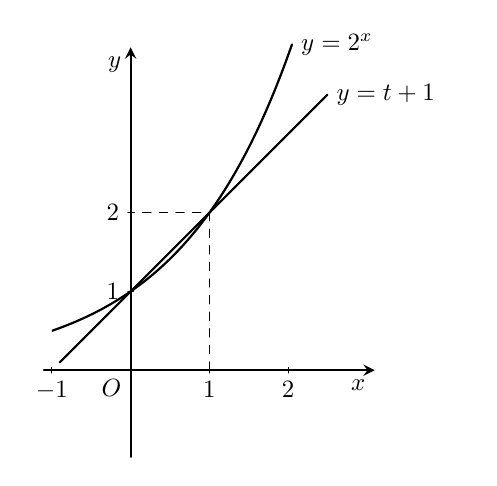
\begin{tikzpicture}[line join=round, line cap=round,>=stealth,thick]
                \tikzset{every node/.style={scale=0.9}}
                \draw[->] (-1.1,0)--(3.1,0) node[below left] {$x$};
                \draw[->] (0,-1.1)--(0,4.1) node[below left] {$y$};
                \draw (0,0) node [below left] {$O$};
                \foreach \x in {-1,1,2}
                \draw[thin] (\x,1pt)--(\x,-1pt) node [below] {$\x$};
                \foreach \y in {1,2}
                \draw[thin] (1pt,\y)--(-1pt,\y) node [left] {$\y$};
                \draw[dashed,thin](1,0)--(1,2)--(0,2);
                \begin{scope}
                    \clip (-1,-1) rectangle (4.3,4.35);
                    \draw[samples=200,domain=-0.9:2.5,smooth,variable=\x] plot (\x,{1*(\x)+1}) node [right] {$y=t+1$};
                    \draw[samples=200,domain=-1:2.05,smooth,variable=\x] plot (\x,{2^(\x)}) node [right] {$y=2^x$};
                \end{scope}
            \end{tikzpicture}
        \end{center}
        Từ đồ thị suy ra $2^t\leq t+1\Leftrightarrow 0\leq t\leq 1\Rightarrow(x-1)^2+y^2\leq 1$. Do đó tập hợp các cặp số $(x;y)$ thỏa mãn thuộc hình tròn $(C)$ tâm $I(1;0),R=1$.\\
        Ta có $P=\dfrac{4y}{2x+y+1}\Leftrightarrow 2Px+(P-4)y+P=0$ là phương trình của đường thẳng $d$.\\
        Do $d$ và $(C)$ có điểm chung $\Leftrightarrow\mathrm{d}\left(I,(d)\right)\leq R\Leftrightarrow\dfrac{|3P|}{\sqrt{4P^2+(P-4)^2}}\leq 1\Leftrightarrow 4P^2+8P-16\leq 0$ \\
        $ \Leftrightarrow-1-\sqrt{5}\leq P\leq-1+\sqrt{5} $, suy ra giá trị nhỏ nhất của $P$ gần nhất với $-3$.
    }
\end{ex}
\begin{ex}%[2D2G3-2]
    Cho các số thực $x, y$ thỏa mãn bất đẳng thức $\log_{4x^2+9y^2}(2x+3y)\geq 1$. Giá trị lớn nhất của biểu thức $P=x+3y$ là
    \choice
    {$\dfrac{3}{2}$}
    {$\dfrac{2+\sqrt{10}}{4}$}
    {$\dfrac{5+\sqrt{10}}{4}$}
    {\True $\dfrac{3+\sqrt{10}}{4}$}
    \loigiai{
        Điều kiện $4x^2+9y^2\neq 1$.\\
        Trường hợp 1: $4x^2+9y^2<1$.\\
        Ta có $(2x)^2+(3y)^2<1\Rightarrow\heva{&2x<1\\&3y<1}\Rightarrow x+3y<\dfrac{1}{2}+1\Rightarrow P<\dfrac{3}{2}$. $(1)$.\\
        Trường hợp 2: $4x^2+9y^2>1$.\\
        Khi đó $\log_{4x^2+9y^2}(2x+3y)\geq 1\Leftrightarrow 2x+3y\geq 4x^2+9y^2\Leftrightarrow\left(2x-\dfrac{1}{2}\right)^2+\left(3y-\dfrac{1}{2}\right)^2\leq\dfrac{1}{2}$.\\
        $P=x+3y=\dfrac{1}{2}\left(2x-\dfrac{1}{2}\right)+\left(3y-\dfrac{1}{2}\right)+\dfrac{3}{4}$.\\
        Áp dụng BĐT Bunhiacopski ta được:\\
        $\left[\dfrac{1}{2}\left(2x-\dfrac{1}{2}\right)+\left(3y-\dfrac{1}{2}\right)\right]^2\leq\left(\dfrac{1}{4}+1\right)\left[\left(2x-\dfrac{1}{2}\right)^2+\left(3y-\dfrac{1}{2}\right)^2\right]\leq\dfrac{5}{8}$.\\
        Suy ra $P=\dfrac{1}{2}\left(2x-\dfrac{1}{2}\right)+\left(3y-\dfrac{1}{2}\right)+\dfrac{3}{4}\leq\dfrac{3+\sqrt{10}}{4}$. $(2)$.\\
        Dấu bằng xảy ra khi và chỉ khi $\heva{&2\left(2x-\dfrac{1}{2}\right)=3y-\dfrac{1}{2}\\&x+3y=\dfrac{3+\sqrt{10}}{4}}\Leftrightarrow\heva{&8x-6y=1\\&4x+12y=3+\sqrt{10}}\Leftrightarrow\heva{&x=\dfrac{5+\sqrt{10}}{20}\\&y=\dfrac{5+2\sqrt{10}}{30}}$. Từ $(1)$ và $(2)$ suy ra giá trị lớn nhất của $P$ là $\dfrac{3+\sqrt{10}}{4}$.
    }
\end{ex}
\begin{ex}%[2D2G3-2]
    [Chuyên Lam Sơn Thanh Hóa 2019]%Câu 28.
    Cho các số thực $a,b$ thay đổi, thỏa mãn $a>\dfrac{1}{3},b>1$. Khi biểu thức $P=\log_{3a}b+\log_b\left(a^4-9a^2+81\right)$ đạt giá trị nhỏ nhất thì tổng $a+b$ bằng
    \choice
    {\True $3+9^{\sqrt{2}}$}
    {$9+2^{\sqrt{3}}$}
    {$2+9\sqrt{2}$}
    {$3+3\sqrt{2}$}
    \loigiai{
        Do $a^4-9a^2+81\geq 9a^2\Leftrightarrow\left(a^2-9\right)^2\geq 0$ đúng $\forall a>\dfrac{1}{3};$ Dấu bằng xảy ra khi $a=3$.\\
        Suy ra $P\geq\log_{3a}b+\log_b(3a)^2=\log_{3a}b+2\log_b3a\geq 2\sqrt{2}$.\\
        Dấu bằng xảy ra khi và chỉ khi $\heva{&a=3\\&\log_{3a}b=2\log_b3a}\Leftrightarrow\heva{&a=3\\&b=9^{\sqrt{2}}.}$ \\
        Vậy, khi $P$ đạt giá trị nhỏ nhất thì $a+b=3+9^{\sqrt{2}}$.
    }
\end{ex}
\begin{ex}%[2D2G3-2]
    [Chuyên Trần Phú Hải Phòng 2019]%Câu 29.
    Cho các số thực $a,b,c$ thỏa mãn $0<a<1;\dfrac{1}{8}<b<1;\dfrac{3}{8}<c<1$. Gọi $M$ là giá trị nhỏ nhất của biểu thức $P=\dfrac{3}{16}\log_a\left(\dfrac{b}{2}-\dfrac{1}{16}\right)+\dfrac{1}{4}\log_b\left(\dfrac{c}{2}-\dfrac{3}{16}\right)+\dfrac{1}{3}\log_ca$. Khẳng định nào sau đây đúng?
    \choice
    {$\sqrt{3}\leq M<2$}
    {$M\geq 2$}
    {\True $\sqrt{2}\leq M<\sqrt{3}$}
    {$M<\sqrt{2}$}
    \loigiai{
        Ta có: $\dfrac{b}{2}-\dfrac{1}{16}=\dfrac{8b-1}{16}=\dfrac{1}{4}\cdot\dfrac{8b-1}{4}\leq\left(\dfrac{2b}{2}\right)^2=b^2$.\\
        $\dfrac{c}{2}-\dfrac{3}{16}=\dfrac{8c-3}{16}=\dfrac{1}{2}\cdot\dfrac{1}{2}\cdot\dfrac{1}{2}\cdot\dfrac{8c-3}{2}\leq\left(\dfrac{4c}{4}\right)^4=c^4$.\\
        Suy ra $P=\dfrac{3}{16}\log_a\left(\dfrac{b}{2}-\dfrac{1}{16}\right)+\dfrac{1}{4}\log_b\left(\dfrac{c}{2}-\dfrac{3}{16}\right)+\dfrac{1}{3}\log_ca$.\\
        $\geq\dfrac{3}{16}\log_ab^2+\dfrac{1}{4}\log_bc^4+\dfrac{1}{3}\log_ac\geq 3\cdot\sqrt[3]{\dfrac{2}{16}}=\dfrac{3}{2}$.\\
        Vậy $P_{\min} =\dfrac{3}{2}\Leftrightarrow\heva{&8b-1=1\\&8c-3=1\\&\dfrac{3}{8}\log_ab=\log_bc=\dfrac{1}{3}\log_ca}\Leftrightarrow\heva{&b=\dfrac{1}{4}\\&c=\dfrac{1}{2}\\&a=\dfrac{\sqrt{2}}{4}}$.
    }
\end{ex}
\begin{ex}%[2D2G3-2]
    Cho các số thực $a,b,m,n$ sao cho $2m+n<0$ và thoả mãn điều kiện:\\
    $\heva{&\log_2\left(a^2+b^2+9\right)=1+\log_2(3a+2b)\\&9^{-m}{\cdot 3}^{-n}{\cdot 3}^{\frac{-4}{2m+n}}+\ln\left[(2m+n+2)^2+1\right]=81.}$ \\
    Tìm giá trị nhỏ nhất của biểu thức $P=\sqrt{(a-m)^2+(b-n)^2}$
    \choice
    {\True $2\sqrt{5}-2$}
    {$2$}
    {$\sqrt{5}-2$}
    {$2\sqrt{5}$}
    \loigiai{
        \begin{itemize}
            \item $\log_2\left(a^2+b^2+9\right)=1+\log_2(3a+2b)\Leftrightarrow a^2+b^2+9=6a+4b\Leftrightarrow a^2+b^2-6a-4b+9=0 (1)$.\\
            Gọi $A(a;b)$. Từ $(1)$ ta suy ra điểm $A$ thuộc điểm đường tròn $(C)$ có tâm $I(3;2)$, bán kính $R=2$.
            \item $9^{-m}\cdot 3^{-n}\cdot 3^{\frac{-4}{2m+n}}+\ln\left[(2m+n+2)^2+1\right]=81\Leftrightarrow\ln\left[(2m+n+2)^2+1\right]=81-3^{-(2m+n)+\dfrac{-4}{2m+n}}(*)$.\\
            Theo bất đẳng thức Cô-si:\\
            $-(2m+n)+\dfrac{-4}{2m+n}\geq 2\sqrt{-(2m+n)\cdot\dfrac{-4}{2m+n}}=4\\
            \Rightarrow 3^{-(2m+n)+\dfrac{-4}{2m+n}}\geq 81$.\\
            (Đẳng thức xảy ra khi: $-(2m+n)=\dfrac{-4}{2m+n}\Rightarrow 2m+n=-2$).\\
            Từ $(*)\Rightarrow\ln\left[(2m+n+2)^2+1\right]\leq 0\Leftrightarrow(2m+n+2)^2+1\leq 1\Leftrightarrow(2m+n+2)^2\leq 0$ \\
            $ \Rightarrow 2m+n+2=0(2) $.
        \end{itemize}
        Gọi $B(m;n)$. Từ $(2)$ ta suy ra điểm $B$ thuộc đường thẳng $\Delta\colon 2x+y+2=0$ \\
        \begin{center}
            \begin{tikzpicture}[line join=round, line cap=round,>=stealth,thick]
                \tikzset{every node/.style={scale=0.9}}
                \draw[->] (-2.4,0)--(5.6,0) node[below left] {$x$};
                \draw[->] (0,-2.6)--(0,4.6) node[below left] {$y$};
                \draw (0,0) node [below left] {$O$};
                \foreach \x in {-2,-1,1,2,3,4,5}
                \draw[thin] (\x,1pt)--(\x,-1pt) node [below] {$\x$};
                \foreach \y in {-1,1,2,3,4}
                \draw[thin] (1pt,\y)--(-1pt,\y) node [left] {$\y$};
                \draw[dashed,thin](3,0)--(3,2)--(0,2);
                \begin{scope}
                    \clip (-2.3,-2.5) rectangle (5.5,4.5);
                    \draw[samples=200,domain=-2.4:0,smooth,variable=\x] plot (\x,{-2*(\x)+-2});
                    \draw[samples=200,domain=-2:5,smooth,variable=\x] plot (\x,{0.5*(\x)+0.5});
                    \coordinate (I) at (3,2);
                    \draw[name path=(C)] (I) circle (2 cm);
                    \coordinate (B) at (-1,0);
                    \draw[name path=BI] (B)--(I);
                    \path [name intersections={of=BI and (C),by={A}}];
                    \foreach \i in {A,B}{\fill[black](\i) circle (1.5pt);}
                    \foreach \i in {A,B,I}{\draw(\i) node[scale=0.9, above]{$\i$};}
                \end{scope}
            \end{tikzpicture}
        \end{center}
        Ta có $P=\sqrt{(a-m)^2+(b-n)^2}=AB$ \\
        $ \Rightarrow\min P=\min AB=\mathrm{d}(I;\Delta)-R=\dfrac{|3\cdot 2+2+2|}{\sqrt{2^2+1^2}}-2=2\sqrt{5}-2 $.
    }
\end{ex}
\begin{ex}%[2D2G3-2]
    Cho các số thực $a,b,c$ thỏa mãn $0<a<1;\dfrac{1}{8}<b<1;\dfrac{3}{8}<c<1$. Gọi $M$ là giá trị nhỏ nhất của biểu thức $P=\dfrac{3}{16}\log_a\left(\dfrac{b}{2}-\dfrac{1}{16}\right)+\dfrac{1}{4}\log_b\left(\dfrac{c}{2}-\dfrac{3}{16}\right)+\dfrac{1}{3}\log_ca$. Khẳng định nào sau đây đúng?
    \choice
    {$\sqrt{3}\leq M<2$}
    {$M\geq 2$}
    {\True $\sqrt{2}\leq M<\sqrt{3}$}
    {$M<\sqrt{2}$}
    \loigiai{
        Ta có: $\dfrac{b}{2}-\dfrac{1}{16}=\dfrac{8b-1}{16}=\dfrac{1}{4}\cdot\dfrac{8b-1}{4}\leq\left(\dfrac{2b}{2}\right)^2=b^2$.\\
        $\dfrac{c}{2}-\dfrac{3}{16}=\dfrac{8c-3}{16}=\dfrac{1}{2}\cdot\dfrac{1}{2}\cdot\dfrac{1}{2}\cdot\dfrac{8c-3}{2}\leq\left(\dfrac{4c}{4}\right)^4=c^4$.\\
        Suy ra $P=\dfrac{3}{16}\log_a\left(\dfrac{b}{2}-\dfrac{1}{16}\right)+\dfrac{1}{4}\log_b\left(\dfrac{c}{2}-\dfrac{3}{16}\right)+\dfrac{1}{3}\log_ca$.\\
        $\geq\dfrac{3}{16}\log_ab^2+\dfrac{1}{4}\log_bc^4+\dfrac{1}{3}\log_ac\geq 3\cdot\sqrt[3]{\dfrac{2}{16}}=\dfrac{3}{2}$.\\
        Vậy $P_{\min} =\dfrac{3}{2}\Leftrightarrow\heva{&8b-1=1\\&8c-3=1\\&\dfrac{3}{8}\log_ab=\log_bc=\dfrac{1}{3}\log_ca}\Leftrightarrow\heva{&b=\dfrac{1}{4}\\&c=\dfrac{1}{2}\\&a=\dfrac{\sqrt{2}}{4}}$.
    }
\end{ex}
\begin{ex}%[2D2G3-2]
    [Chuyên Lam Sơn - 2020]%Câu 32.
    Xét các số thực dương $a,b,c$ lớn hơn $1$ (với $a>b$) thỏa mãn $4\left(\log_ac+\log_bc\right)=25\log_{ab}c$. Giá trị nhỏ nhất của biểu thức $\log_ba+\log_ac+\log_cb$ bằng
    \choice
    {\True $5$}
    {$8$}
    {$\dfrac{17}{4}$}
    {$3$}
    \loigiai{
        Đặt $\log_ca=x,\log_cb=y$.\\
        Vì $a,b,c>1$ và $a>b$ nên suy ra $\log_ca>\log_cb$ hay $x>y>0$.\\
        Từ giả thiết suy ra: $4\left(\dfrac{1}{\log_ca}+\dfrac{1}{\log_cb}\right)=25\cdot\dfrac{1}{\log_cab}\Leftrightarrow\dfrac{4}{x}+\dfrac{4}{y}=\dfrac{25}{x+y}$ \\
        $ \Leftrightarrow\dfrac{(x+y)^2}{xy}=\dfrac{25}{4}\Leftrightarrow\dfrac{x}{y}+\dfrac{y}{x}=\dfrac{17}{4}\Rightarrow\hoac{&\dfrac{x}{y}=4\\&\dfrac{x}{y}=\dfrac{1}{4}}\Rightarrow x=4y $ (vì $x>y$).\\
        Ta có: $\log_ba+\log_ac+\log_cb=\dfrac{\log_ca}{\log_cb}+\dfrac{1}{\log_ca}+\log_cb =\dfrac{x}{y}+\dfrac{1}{x}+y$.\\
        $=\dfrac{x}{y}+\dfrac{1}{4y}+y\geq 4+2\sqrt{\dfrac{1}{4y}\cdot y}=5$.\\
        Dấu bằng xảy ra khi và chỉ khi $y=\dfrac{1}{2}$ và $x=2$, tức là $a=c^2;c=b^2$.\\
        Vậy giá trị nhỏ nhất của biểu thức đã cho bằng $5$.\\
        Cách khác.\\
        Từ giả thiết suy ra: $4\left(\log_ab\cdot\log_bc+\log_bc\right)=25\cdot\log_{ab}b\cdot\log_bc$ \\
        $ \Leftrightarrow 4\log_bc(\log_ab+1)=25\dfrac{\log_bc}{\log_bab}\Leftrightarrow\hoac{&\log_bc=0\\&4(\log_ab+1)=\dfrac{25}{\log_ba+1}.} $ \\
        Do $a,b,c>1$ nên $\log_bc>0$; suy ra $4(1+\log_ab)(1+\log_ba)=25\Rightarrow\log_ab=\dfrac{1}{4}$.\\
        Khi đó: $\log_ba+\log_ac+\log_cb\geq 4+2\sqrt{\log_ac\cdot\log_cb}=4+2\sqrt{\log_ab}=5$.\\
        Vậy giá trị nhỏ nhất của biểu thức bằng $5$ đạt được khi và chỉ khi $a=b^4,a=c^2,c=b^2$.
    }
\end{ex}
\begin{ex}%[2D2G3-2]
    [Chuyên Lương Văn Tỵ - Ninh Bình - 2020]%Câu 33.
    Xét các số thực dương $a$, $b$, $x$, $y$ thỏa mãn $a>1$, $b>1$ và $a^{2x}=b^{3y}=a^6b^6$. Biết giá trị nhỏ nhất của biểu thức $P=4xy+2x-y$ có dạng $m+n\sqrt{165}$ (với $m,n$ là các số tự nhiên), tính $S=m+n$.
    \choice
    {$58$}
    {$54$}
    {\True $56$}
    {$60$}
    \loigiai{
        Theo bài ra ta có $a^{2x}=b^{3y}=a^6b^6\Leftrightarrow\heva{&a^{2x}=a^6b^6\\&b^{3y}=a^6b^6}\Leftrightarrow\heva{&2x=\log_a\left(a^6b^6\right)\\&3y=\log_b\left(a^6b^6\right)}\Leftrightarrow\heva{&2x=6+6\log_ab\\&3y=6+6\log_ba}$ \\
        $ \Leftrightarrow\heva{&x=3(1+\log_ab)\\&y=2(1+\log_ba).} $ \\
        Vì $a$, $b>1$ nên $\log_ab>\log_a1=0$.\\
        Do đó:\\
        .\\
        $P=4xy+2x-y=24(1+\log_ab)(1+\log_ba)+6+6\log_ab-2-2\log_ba$.\\
        $=52+30\log_ab+22\log_ba\geq 52+2\sqrt{30\log_ab\cdot 22\log_ba}=52+4\sqrt{165}$.\\
        Vậy $P$ đạt giá trị nhỏ nhất là $m+n\sqrt{165}$ khi $30\log_ab=22\log_ba\Leftrightarrow\log_ab=\sqrt{\dfrac{11}{15}}\Leftrightarrow b=a^{\sqrt{\frac{11}{15}}}$.\\
        Ta có: $\heva{&m=52\\&n=4}\Rightarrow m+n=56$.}
\end{ex}
\begin{ex}%[2D2G3-2]
    [Chuyên Lê Hồng Phong - Nam Định - 2020]%Câu 34.
    Xét các số thực $x, y$ thỏa mãn $\log_2(x-1)+\log_2(y-1)=1$. Khi biểu thức $P=2x+3y$ đạt giá trị nhỏ nhất thì $3x-2y=a+b\sqrt{3}$ với $a, b\in\mathbb{Q}$. Tính $T=ab$?
    \choice
    {$T=9$}
    {$T=\dfrac{7}{3}$}
    {\True $T=\dfrac{5}{3}$}
    {$T=7$}
    \loigiai{
        Điều kiện: $\heva{&x-1>0\\&y-1>0}\Leftrightarrow\heva{&x>1\\&y>1.}$ \\
        Khi đó: $\log_2(x-1)+\log_2(y-1)=1\Leftrightarrow(x-1)(y-1)=2\Leftrightarrow y-1=\dfrac{2}{x-1}\Leftrightarrow y=\dfrac{2}{x-1}+1$.\\
        Suy ra: $P=2x+3y=2x+\dfrac{6}{x-1}+3=2(x-1)+\dfrac{6}{x-1}+5$.\\
        Cách 1: Dùng bất đẳng thức.\\
        Áp dụng bất đẳng thức Côsi, ta có: $2(x-1)+\dfrac{6}{x-1}\geq 2\sqrt{2(x-1)\cdot\dfrac{6}{x-1}}$ \\
        $ \Rightarrow 2(x-1)+\dfrac{6}{x-1}\geq 4\sqrt{3}\Rightarrow P\geq 4\sqrt{3}+5 $.\\
        Dấu ``$=$'' xảy ra $\Leftrightarrow 2(x-1)=\dfrac{6}{x-1}\Leftrightarrow(x-1)^2=3\Leftrightarrow|x-1|=\sqrt{3}\Leftrightarrow\hoac{&x=1+\sqrt{3}(\mathrm{N})\\&x=1-\sqrt{3}(\mathrm{L})}$ \\
        $ \Rightarrow y=\dfrac{2}{\sqrt{3}}+1=\dfrac{2\sqrt{3}+3}{3} $.\\
        Do đó: $3x-2y=3(1+\sqrt{3})-2\left(\dfrac{2\sqrt{3}+3}{3}\right)=1+\dfrac{5}{3}\sqrt{3}\Rightarrow a=1; b=\dfrac{5}{3}\Rightarrow T=ab=\dfrac{5}{3}$.\\
        Cách 2: Dùng bảng biến thiên.\\
        Ta có $P=2x+\dfrac{6}{x-1}+3\Rightarrow P’=2-\dfrac{6}{(x-1)^2}$.\\
        $P’=0\Leftrightarrow\hoac{&x=1+\sqrt{3}(\mathrm{N})\\&x=1-\sqrt{3}(\mathrm{L}).}$ \\
        Bảng biến thiên
        \begin{center}
            
\begin{tikzpicture}
                \tkzTabInit[nocadre,lgt=1,espcl=3]{$x$/0.8,$P'$/0.8,$P$/2.5}{$1$,$1+\sqrt{3}$,$+\infty$}
                \tkzTabLine{,-,0,+,}
                \tkzTabVar{+/$+\infty$,-/$4\sqrt{3}+5$,+/$+\infty$}
            \end{tikzpicture}
        \end{center}
        Dựa vào bảng biến thiên, ta có $P_{\min} =4\sqrt{3}+5\Leftrightarrow x=1+\sqrt{3}\Rightarrow y=\dfrac{2\sqrt{3}+3}{3}$.\\
        Do đó: $3x-2y=3(1+\sqrt{3})-2\left(\dfrac{2\sqrt{3}+3}{3}\right)=1+\dfrac{5}{3}\sqrt{3}\Rightarrow a=1; b=\dfrac{5}{3}\Rightarrow T=ab=\dfrac{5}{3}$.
    }
\end{ex}
\begin{ex}%[2D2G3-2]
    [Chuyên Sơn La - 2020]%Câu 35.
    Cho $a,b,c$ là các số thực lớn hơn $1$. Giá trị nhỏ nhất của biểu thức $P=\dfrac{4040}{\log_{\sqrt{bc}}a}+\dfrac{1010}{\log_{ac}\sqrt{b}}+\dfrac{8080}{3\log_{ab}\sqrt[3]{c}}$ bằng
    \choice
    {$2020$}
    {$16160$}
    {\True $20200$}
    {$13130$}
    \loigiai{
        Ta có $P=\dfrac{4040}{\log_{\sqrt{bc}}a}+\dfrac{1010}{\log_{ac}\sqrt{b}}+\dfrac{8080}{3\log_{ab}\sqrt[3]{c}}=\dfrac{4040}{2\log_{bc}a}+\dfrac{1010}{\frac{1}{2}\log_{ac}b}+\dfrac{8080}{3\cdot\frac{1}{3}\log_{ab}c}$.\\
        $=2020\log_abc+2020\log_bac+8080\log_cab$.\\
        $=2020\left(\log_ab+\log_ac\right)+2020\left(\log_ba+\log_bc\right)+8080\left(\log_ca+\log_cb\right)$.\\
        $=2020\log_ab+2020\log_ba+2020\log_ac+8080\log_ca+2020\log_bc+8080\log_cb$.\\
        Vì $a,b,c>1$ nên các số $\log_ab,\log_ba,\log_ac,\log_ca,\log_bc,\log_cb>0$.\\
        Khi đó ta có\\
        $2020\log_ab+2020\log_ba\geq 2\sqrt{2020^2\log_ab\log_ba}=4040$.\\
        $2020\log_ac+8080\log_ca\geq 2\sqrt{4040^2\log_ac\log_ca}=8080$.\\
        $2020\log_bc+8080\log_cb\geq 2\sqrt{4040^2\log_bc\log_cb}=8080$.\\
        Suy ra $P\geq 4040+8080+8080=20200$.
    }
\end{ex}
\begin{ex}%[2D2G3-2]
    [Chuyên Vĩnh Phúc - 2020]%Câu 36.
    Cho $a,b,c$ là các số thực dương khác $1$ thỏa mãn $\log_a^2b+\log_b^2c=\log_a\dfrac{c}{b}-2\log_b\dfrac{c}{b}-3$. Gọi $M,m$ lần lượt là giá trị lớn nhất, giá trị nhỏ nhất của $P=\log_ab-\log_bc$. Giá trị của biểu thức $S=3m-M$ bằng
    \choice
    {$-16$}
    {$4$}
    {\True $-6$}
    {$6$}
    \loigiai{
        Biến đổi đẳng thức đề bài ta được.\\
        $\begin{aligned}&\log_a^2b+\log_b^2c=\log_a\dfrac{c}{b}-2\log_b\dfrac{c}{b}-3\Leftrightarrow\log_a^2b+\log_b^2c=\log_ac-\log_ab-2\log_bc-1\\&\Leftrightarrow\log_a^2b+\log_b^2c=\log_ab\cdot\log_bc-\log_ab-2\log_bc-1.\end{aligned}$\\
        Đặt $u=\log_ab;v=\log_bc$ ta có phương trình.\\
        $u^2+v^2=uv-u-2v-1$ \\
        $ \Leftrightarrow u^2-2uv+v^2+u^2+2u+1+v^2+4v+4=3 $ \\
        $ \Leftrightarrow (u-v)^2+(u+1)^2+(v+2)^2=3 (*) $.\\
        Ta có bất đẳng thức quen thuộc $x^2+y^2\geq\dfrac{1}{2}(x-y)^2$ dấu bằng xảy ra khi $x=-y$, áp dụng bất đẳng thức này ta có\\
        $(u+1)^2+(v+2)^2\geq\dfrac{1}{2}(u+1-v-2)^2\Leftrightarrow (u+1)^2+(v+2)^2\geq\dfrac{1}{2}(u-v-1)^2$ (**).\\
        Từ (*) và (**) ta có $3-(u-v)^2\geq\dfrac{1}{2}(u-v-1)^2$ hay.\\
        $3-P^2\geq\dfrac{1}{2}(P-1)^2\Leftrightarrow 3P^2-2P-5\leq 0\Leftrightarrow-1\leq P\leq\dfrac{5}{3}$.\\
        Vậy $m=-1,M=\dfrac{5}{3}$ suy ra $S=m-3M=-6$.
    }
\end{ex}
\begin{ex}%[2D2G3-2]
    [Sở Hưng Yên - 2020]%Câu 37.
    Cho các số thực $x,y\geq 1$ và thỏa mãn điều kiện $xy\leq 4$. Biểu thức $P=\log_{4x}8x-\log_{2y^2}\dfrac{y^2}{2}$ đạt giá trị nhỏ nhất tại $x=x_0,y=y_0$. Đặt $T=x_0^4+y_0^4$ mệnh đề nào sau đây đúng
    \choice
    {$T=131$}
    {$T=132$}
    {$T=129$}
    {\True $T=130$}
    \loigiai{
        Ta có $P=\log_{4x}8x-\log_{2y^2}\dfrac{y^2}{2} =\dfrac{\log_28x}{\log_24x}-\dfrac{\log_2\dfrac{y^2}{2}}{\log_22y^2} =\dfrac{3+\log_2x}{2+\log_2x}-\dfrac{2\log_2y-1}{2\log_2y+1}$.\\
        Đặt $\log_2x=a$, $\log_2y=b$ ($a,b\geq 0$), ta được $P=\dfrac{3+a}{2+a}-\dfrac{2b-1}{2b+1} =\dfrac{1}{2+a}+\dfrac{2}{2b+1}$.\\
        Vì $xy\leq 4$ suy ra $\log_2x+\log_2y\leq 2\Leftrightarrow a+b\leq 2\Leftrightarrow 0\leq a\leq 2-b$.\\
        Suy ra $P=\dfrac{1}{2+a}+\dfrac{2}{2b+1}\geq\dfrac{1}{4-b}+\dfrac{2}{2b+1}$.\\
        Xét hàm $f(b)=\dfrac{1}{4-b}+\dfrac{2}{2b+1}$ trên $[0;2]$,ta có:\\
        $f’(b)=\dfrac{1}{(4-b)^2}-\dfrac{4}{(2b+1)^2}$.\\
        $f’(b)=0\Leftrightarrow(2b+1)^2-4(4-b)^2=0\Leftrightarrow b=\dfrac{7}{4}$.\\
        Ta có: $f(0)=\dfrac{9}{4},f(2)=\dfrac{9}{10},f\left(\dfrac{7}{4}\right)=\dfrac{8}{9}$.\\
        Suy ra trên đoạn $[0;2]$ ta có: $\min P=\dfrac{8}{9}\Leftrightarrow\heva{&\log_2x=\dfrac{1}{4}\\&\log_2y=\dfrac{7}{4}}\Leftrightarrow\heva{&x=2^{\frac{1}{4}}\\&y=2^{\frac{7}{4}}}\Rightarrow\heva{&x_0=2^{\frac{1}{4}}\\&y_0=2^{\frac{7}{4}}.}$ \\
        Vậy $T=x_0^4+y_0^4=\left(2^{\frac{1}{4}}\right)^4+\left(2^{\frac{7}{4}}\right)^4=130$.
    }
\end{ex}
\begin{ex}%[2D2G3-2]
    [Sở Hà Tĩnh - 2020]%Câu 38.
    Cho các số thực dương $a,b,c$ thỏa mãn $abc=10$. Biết giá trị lớn nhất của biểu thức $F=5\log a\cdot\log b+2\log b\cdot\log c+\log c\cdot\log a$ bằng $\dfrac{m}{n}$ với $m,n$ nguyên dương và $\dfrac{m}{n}$ tối giản. Tổng $m+n$ bằng
    \choice
    {$13$}
    {$16$}
    {\True $7$}
    {$10$}
    \loigiai{
        Đặt $\heva{&\log a=x\\&\log b=y\\&\log c=z}\Rightarrow\heva{&a={10}^x\\&b={10}^y\\&c={10}^z}$, mà $abc=10\Leftrightarrow 10^x\cdot 10^y\cdot 10^z=10\Leftrightarrow x+y+z=1(*)$.\\
        Ta có $F=5\log a\cdot\log b+2\log b\cdot\log c+\log c\cdot\log a=5xy+2yz+zx$.\\
        Từ $(*)\Rightarrow y=1-x-z$, thay vào biểu thức $F$, ta được:\\
        $F=5x(1-x-z)+2(1-x-z)z+xz=-2z^2-5x^2-6xz+2z+5x$.\\
        $=-2z^2-\dfrac{9}{2}x^2-\dfrac{1}{2}-6xz+2z+3x-\dfrac{1}{2}x^2+2x-2+\dfrac{5}{2}$.\\
        $=-2\left(z^2+\dfrac{9}{4}x^2+\dfrac{1}{4}+3xz-z-\dfrac{3}{2}x\right)-\dfrac{1}{2}\left(x^2-4x+4\right)+\dfrac{5}{2}$.\\
        $=-2\left(z+\dfrac{3}{2}x-\dfrac{1}{2}\right)^2-\dfrac{1}{2}(x-2)^2+\dfrac{5}{2}\leq\dfrac{5}{2}$.\\
        Vậy $\max F=\dfrac{5}{2}$ khi và chỉ khi $\heva{&x+y+z=1\\&z+\dfrac{3}{2}x-\dfrac{1}{2}=0\\&x-2=0}\Leftrightarrow\heva{&y=\dfrac{3}{2}\\&x=2\\&z=-\dfrac{5}{2}.}$ \\
        Vậy $m=5,n=2\Rightarrow m+n=5+2=7$.
    }
\end{ex}
\begin{ex}%[2D2G3-2]
    [Liên trường Nghệ An - 2020]%Câu 39.
    Cho các số thực dương $a;b;c$ khác $1$ thỏa mãn $\log_a^2b+\log_b^2c+2\log_b\dfrac{c}{b}=\log_a\dfrac{c}{a^3b}$. Gọi $M,m$ lần lượt là giá trị lớn nhất và giá trị nhỏ nhất của $P=\log_aab-\log_bbc$. Tính giá trị biểu thức $S=2m^2+9M^2$.
    \choice
    {$S=28$}
    {$S=25$}
    {$S=26$}
    {\True $S=27$}
    \loigiai{
        Đặt $x=\log_ab;y=\log_bc,(x;y>0)\Rightarrow\log_ac=xy\Rightarrow P=\log_aab-\log_bbc=x-y\Rightarrow x=P+y$.\\
        Khi đó ta có $\begin{aligned}&\log_a^2b+\log_b^2c+2\log_b\dfrac{c}{b}=\log_a\dfrac{c}{a^3b}\Leftrightarrow x^2+y^2+2y-2=xy-3-x\\&(P+y)^2+y^2+2y-2=(P+y)y-3-(P+y)\\&\Leftrightarrow y^2+(P+3)y+P^2+P+1=0.\end{aligned}$\\
        Phương trình có nghiệm khi $\Delta\geq 0\Leftrightarrow-3P^2+2P+5\geq 0\Leftrightarrow-1\leq P\leq\dfrac{5}{3}\Rightarrow m=-1;M=\dfrac{5}{3}\Rightarrow S=27$.\\
        Nên giá trị nhỏ nhất của $P$ là $\dfrac{8}{9}\Leftrightarrow\heva{&\log_2x=\dfrac{1}{4}\\&\log_2y=\dfrac{7}{4}}\Leftrightarrow\heva{&x=2^{\frac{1}{4}}\\&y=2^{\frac{7}{4}}}\Rightarrow\heva{&x_0=2^{\frac{1}{4}}\\&y_0=2^{\frac{7}{4}}}\Rightarrow T=x_0^4+y_0^4=130$.
    }
\end{ex}
\begin{ex}%[2D2G3-2]
    [Nguyễn Huệ - Phú Yên - 2020]%Câu 40.
    Xét các số thực $a,b,x,y$ thỏa mãn $a>1,b>1$ và $a^x=b^y=\sqrt{\dfrac{a}{b}}$. Giá trị lớn nhất của biểu thức $P=x-2y$ thuộc tập nào dưới đây?
    \choice
    {\True $\left(0;\dfrac{1}{2}\right)$}
    {$\left(-1;-\dfrac{1}{2}\right)$}
    {$\left[1;\dfrac{3}{2}\right)$}
    {$\left[\dfrac{3}{2};\dfrac{5}{2}\right)$}
    \loigiai{
        Từ giả thiết ta có $\heva{&a^x=\sqrt{\dfrac{a}{b}}\\&b^y=\sqrt{\dfrac{a}{b}}}\Leftrightarrow\heva{&x=\log_a\sqrt{\dfrac{a}{b}}\\&y=\log_b\sqrt{\dfrac{a}{b}}}\Leftrightarrow\heva{&x=\dfrac{1}{2}(1-\log_ab)\\&y=\dfrac{1}{2}\left(\dfrac{1}{\log_ab}-1\right).}$ \\
        Đặt $t=log_ab$. Vì $a>1,b>1$, nên $t>0$.\\
        Khi đó: $P=\dfrac{1}{2}(1-t)-\left(\dfrac{1}{t}-1\right)=\dfrac{3}{2}-\dfrac{t}{2}-\dfrac{1}{t}=\dfrac{3}{2}-\left(\dfrac{t}{2}+\dfrac{1}{t}\right)\leq\dfrac{3}{2}-2\cdot\sqrt{\dfrac{t}{2}\cdot\dfrac{1}{t}}=\dfrac{3-2\sqrt{2}}{2}$.\\
        Dấu bằng xảy ra khi và chỉ khi $\dfrac{t}{2}=\dfrac{1}{t}\Leftrightarrow t=\sqrt{2}(t>0)$. $P_{\max} =\dfrac{3-2\sqrt{2}}{2}\approx 0,086\in\left(0;\dfrac{1}{2}\right)$.
    }
\end{ex}
\begin{ex}%[2D2G3-2]
    [Tiên Du - Bắc Ninh - 2020]%Câu 41.
    Cho biểu thức $P=3^{y-2x+3}(1+4^{2x-y-1})-2^{2x-y-1}$ và biểu thức $Q=\log_{y-3-2x}3y$. Giá trị nhỏ nhất của y để tồn tại $x$ đồng thời thỏa mãn $P\geq 1$ và $Q\geq 1$ là số $y_0$. Khẳng định nào sau đây là đúng?
    \choice
    {\True $4y_0+1$ là số hữu tỷ}
    {$y_0$ là số vô tỷ}
    {$y_0$ là số nguyên dương}
    {$3y_0+1$ là số tự nhiên chẵn}
    \loigiai{
        Điều kiện $\heva{&y-2x+3>0\\&y>0.}$ \\
        $P=3^{y-2x+1}\cdot (1+4^{2x-y-1})-2^{2x-y-1}=3^{y-2x+1}\cdot (1+\dfrac{1}{4^{2x-y-1}})-\dfrac{1}{2^{y-2x+1}}$.\\
        Đặt $t=y-2x+1$ ta có $P=3^t(1+\dfrac{1}{4^t})-\dfrac{1}{2^t}$.\\
        Cho $P\geq 1\Leftrightarrow 3^t(1+\dfrac{1}{4^t})-\dfrac{1}{2^t}\geq 1\Leftrightarrow 12^t+3^t\geq 4^t+2^t(1)$.\\
        Với $t=0$ thỏa mãn (1).\\
        Với $t>0$ ta có $\heva{&{12}^t>4^t\\&3^t>2^t}\Rightarrow 12^t+3^t>4^t+2^t\Rightarrow (1)$ thỏa mãn.\\
        Với $t<0$ ta có $\heva{&{12}^t<4^t\\&3^t<2^t}\Rightarrow 12^t+3^t<4^t+2^t\Rightarrow (1)$ không thỏa mãn.\\
        Vậy $(1)\Leftrightarrow t\geq 0$ hay $y-2x+1\geq 0$ (a).\\
        Vì $y-2x+1>0\Rightarrow y-2x+3>2>1$ nên $Q=\log_{y-2x+1}3y\geq 1\Leftrightarrow 3y\geq y-2x+3\Leftrightarrow 2x+2y\geq 3$ (b).\\
        Từ (a), (b) và điều kiện ta có $\heva{&y-2x+1\geq 0\\&2x+2y\geq 3\\&y>0.}$ \\
        Cặp số $(x;y)$ thỏa mãn hệ được biểu diễn ở miền không bị gạch ở hình bên. Điểm A thuộc miền không bị gạch và có $y_{\min} =\dfrac{2}{3}$. \\
        \begin{center}
            \begin{tikzpicture}[line join=round, line cap=round,>=stealth,thick, scale=2]
                \clip (-1,-1.5) rectangle (2,2);
                \fill[pattern=north east lines] (-2,-5)--(3,-5)--(3,5)--cycle;
                \fill[pattern=north west lines] (-2,3.5)--(-2,-2.5)--(4,-2.5)--cycle;
                \fill[pattern=horizontal lines] (-1,0)--(-1,-1.5)--(2,-1.5)--(2,0)--cycle;
                \draw (1.5,2)--(-0.25,-1.5);
                \draw (-0.5,2)--(3,-1.5);
                \draw[->] (-1,0)--(2,0) node[below]{$x$};
                \draw[->] (0,-1.5)--(0,2) node[below left]{$y$};
                \draw (0,0) node[below left]{$O$};
                \draw[thin] (0.8333333333,1pt)--(0.8333333333,-1pt) node [below] {$\frac{5}{6}$};
                \draw[thin] (1.5,1pt)--(1.5,-1pt) node [below] {$\frac{3}{2}$};
                \draw[thin] (1pt,0.6666666667)--(-1pt,0.6666666667) node [left] {$\frac{2}{3}$};
                \draw[thin] (1pt,1.5)--(-1pt,1.5) node [left] {$\frac{3}{2}$};
                \draw[dashed,thin] (0.8333333333,0)--(0.8333333333,0.6666666667)--(0,0.6666666667);
            \end{tikzpicture}
        \end{center}
        Vậy $y_0=\dfrac{2}{3}$. Do đó $4y_0+1=\dfrac{11}{3}\in\mathbb{Q}$.
    }
\end{ex}
\begin{ex}%[2D2G3-2]
    [Trường VINSCHOOL - 2020]%Câu 42.
    Cho dãy số $(u_n)$ có số hạng đầu $u_1\neq 1$ thỏa mãn $\log_2^2(5u_1)+\log_2^2(7u_1)=\log_2^25+\log_2^27$ và $u_{n+1}=7u_n$ với mọi $n\geq 1$. Giá trị nhỏ nhất của $n$ để $u_n>1111111$ bằng
    \choice
    {$11$}
    {$8$}
    {$9$}
    {\True $10$}
    \loigiai{
        Ta có $u_{n+1}=7u_n,\forall n\geq 1\Rightarrow(u_n)$ là một cấp số nhân với số hạng đầu là $u_1$, công bội $q=7$.\\
        $\log_2^2(5u_1)+\log_2^2(7u_1)=\left[\log_25+\log_2u_1\right]^2+\left[\log_27+\log_2u_1\right]^2$.\\
        $=\log_2^25+2\cdot\log_25\cdot\log_2u_1+\log_2^2u_1+\log_2^27+2\cdot\log_27\cdot\log_2u_1+\log_2^2u_1$.\\
        $=2\log_2^2u_1+2\cdot\left(\log_25+\log_27\right)\cdot\log_2u_1+\log_2^25+\log_2^27$.\\
        $=2\log_2^2u_1+2\cdot\log_235\cdot\log_2u_1+\log_2^25+\log_2^27=\log_2^25+\log_2^27$ \\
        $ \Leftrightarrow 2\log_2^2u_1+2\cdot\log_235\cdot\log_2u_1=0\Leftrightarrow 2\log_2u_1\cdot\left(\log_2u_1+\log_235\right)=0 $ \\
        $ \Leftrightarrow\hoac{&\log_2u_1=0\\&\log_2u_1+\log_235=0}\Leftrightarrow\hoac{&u_1=1(loai)\\&\log_2u_1=-\log_235}\Leftrightarrow u_1=\dfrac{1}{35}\quad(nhan) $.\\
        Số hạng tổng quát của dãy số là $u_n=u_1\cdot q^{n-1}=\dfrac{1}{35}\cdot 7^{n-1}=\dfrac{1}{5\cdot 7}\cdot 7^{n-1}=\dfrac{1}{5}\cdot 7^{n-2}$.\\
        $u_n>1111111\Leftrightarrow\dfrac{1}{5}\cdot 7^{n-2}>1111111\Leftrightarrow 7^{n-2}>5555555\Leftrightarrow n-2>\log_75555555$ \\
        $ \Leftrightarrow n>\log_75555555+2 $. Vì $n\in\mathbb{N}^{*}$ nên giá trị nhỏ nhất của $n$ bằng $10$.
    }
\end{ex}
\begin{ex}%[2D2G3-2]
    [Chuyên Lê Hồng Phong - Nam Định - 2020]%Câu 43.
    Xét các số thực $x,y$ thỏa mãn $\log_2(x-1)+\log_2(y-1)=1$. Khi biểu thức $P=2x+3y$ đạt giá trị nhỏ nhất thì $3x-2y=a+b\sqrt{3}$ với $a,b\in\mathbb{Q}$. Tính $T=ab$.
    \choice
    {$T=9$}
    {$T=\dfrac{7}{3}$}
    {\True $T=\dfrac{5}{3}$}
    {$T=7$}
    \loigiai{
        Ta có $\log_2(x-1)+\log_2(y-1)=1\Leftrightarrow\heva{&x,y>1\\&y-1=\dfrac{2}{x-1}}\Leftrightarrow\heva{&x>1\\&y=1+\dfrac{2}{x-1}.}$ \\
        Khi đó $P=2x+3y=2x+3\left(\dfrac{2}{x-1}+1\right)=2(x-1)+\dfrac{6}{x-1}+5\geq 2\sqrt{12}+5$, dấu bằng xảy ra khi và chỉ khi\\
        $\heva{&x>1\\&2(x-1)=\dfrac{6}{x-1}\\&y=1+\dfrac{2}{x-1}}\Leftrightarrow\heva{&x-1=\sqrt{3}\\&y=1+\dfrac{2}{\sqrt{3}}}\Rightarrow 3x-2y=3(1+\sqrt{3})-2\left(1+\dfrac{2}{\sqrt{3}}\right)=1+\dfrac{5\sqrt{3}}{3.}$ \\
        Vậy $a=1,b=\dfrac{5}{3}$ nên $T=\dfrac{5}{3}$.
    }
\end{ex}
\begin{ex}
    Xét các số thực $a$, $b$, $c\neq 0$ thỏa mãn $3^a=5^b=15^{-c}$. Giá trị nhỏ nhất của biểu thức $P=a^2+b^2+c^2-4(a+b+c)$ thuộc tập hợp nào dưới đây?
    \choice
    {$(-1;2)$}
    {\True $[-5;-1)$}
    {$[2;4)$}
    {$[4;6)$}
    \loigiai{
        Đặt $3^a=5^b=15^{-c}=t>0\Rightarrow\heva{&a=\log_3t\\&b=\log_5t\\&c=-\log_{15}t}$. Khi đó\\
        $P=\log_3^2t+\log_5^2t+\log_{15}^2t-4(\log_3t+\log_5t-\log_{15}t)$.\\
        $=\log_3^2t\left(1+\log_5^23+\log_{15}^23\right)-4\log_3t\left(1+\log_53-\log_{15}3\right)$.\\
        $=X^2\left(1+\log_5^23+\log_{15}^23\right)-4X\left(1+\log_53-\log_{15}3\right)$, (với $X=\log_3t$).\\
        $P_{\min} =\mathrm{P}\left(\dfrac{2\left(1+\log_53-\log_{15}3\right)}{1+\log_5^23+\log_{15}^23}\right)=-4$,\\
        khi $\log_3t=\dfrac{2\left(1+\log_53-\log_{15}3\right)}{1+\log_5^23+\log_{15}^23}\Rightarrow t=3^{\frac{2\left(1+\log_53-\log_{15}3\right)}{1+\log_5^23+\log_{15}^23}}$.\\
        Suy ra.\\
        $\begin{aligned}&a=\dfrac{2\left(1+\log_53-\log_{15}3\right)}{1+\log_5^23+\log_{15}^23}\\&b=\log_53^{\frac{2\left(1+\log_53-\log_{15}3\right)}{1+\log_5^23+\log_{15}^23}}\\&c=-\log_{15}3^{\frac{2\left(1+\log_53-\log_{15}3\right)}{1+\log_5^23+\log_{15}^23}}.\end{aligned}$.
    }
\end{ex}
\begin{ex}%[2D2G3-2]
    Xét các số thực dương $a$, $b$, $c$, $x$, $y$, $z$ thỏa mãn $a>1$, $b>1$, $c>1$ và $a^x=b^y=c^z=\sqrt{abc}$. Giá trị nhỏ nhất của biểu thức $P=x+y+z+\dfrac{1}{2}$ thuộc tập hợp nào dưới đây?
    \choice
    {$[10;13)$}
    {$[7;10)$}
    {$[3;5)$}
    {\True $[5;7)$}
    \loigiai{
        Từ giả thiết ta có\\
        $x=\dfrac{1}{2}\left(1+\log_ab+\log_ac\right)$, $y=\dfrac{1}{2}\left(1+\log_ba+\log_bc\right)$, $z=\dfrac{1}{2}\left(1+\log_cb+\log_ca\right)$. Khi đó ta có\\
        $2P=4+\log_ab+\log_ba+\log_ac+\log_ca+\log_bc+\log_cb$.\\
        Vì $a>1$, $b>1$, $c>1$ nên $\log_ab>0$, $\log_bc>0$, $\log_ca>0$, $\log_ba>0$, $\log_cb>0$, $\log_ac>0$.\\
        Áp dụng bất đẳng thức Cô Si ta được.\\
        $\log_ab+\log_ba\geq 2\sqrt{\log_ab\cdot\log_ba}$ hay $\log_ab+\log_ba\geq 2$.\\
        Tương tự $\log_ac+\log_ca\geq 2$ và $\log_bc+\log_cb\geq 2$.\\
        Do đó $2P\geq 10$ hay $P\geq 5$. Dấu xảy ra khi và chỉ khi $a=b=c$.\\
        Vậy giá trị nhỏ nhất $P_{\min} =5$.
    }
\end{ex}
\begin{ex}%[2D2G3-2]
    Xét các số thực dương $a,b,x,y$ thỏa mãn $a>1,b>1$ và $a^{x^2}=b^{y^2}=\sqrt{a\cdot b}$. Giá trị nhỏ nhất của biểu thức $P=x\cdot y$ là
    \choice
    {$P=\dfrac{9}{4}$}
    {\True $P=\dfrac{\sqrt{6}}{2}$}
    {$P=\dfrac{3}{2}$}
    {$P=\dfrac{4}{9}$}
    \loigiai{
        $a^{x^2}=b^{y^2}=\sqrt{a\cdot b}\Leftrightarrow\heva{&x^2=\dfrac{1}{2}\log_ab+\dfrac{1}{2}\\&y^2=\dfrac{1}{2}\log_ba+\dfrac{1}{2}.}$ \\
        $(xy)^2=\left(\dfrac{1}{2}\log_ab+\dfrac{1}{2}\right)\left(\dfrac{1}{2}\log_ba+\dfrac{1}{2}\right) =\left(\dfrac{1}{4}+\dfrac{1}{2}\left(\log_ab+\log_ba\right)+\dfrac{1}{4}\right)$.\\
        $\geq\dfrac{3}{2}$ ($a,b>1\Rightarrow\log_ab>0,\log_ba>0$).\\
        Vì $x>0,y>0\Rightarrow xy\geq\dfrac{\sqrt{6}}{2}$. Dấu bằng xảy ra khi và chỉ khi $a=b$.
    }
\end{ex}
\begin{ex}%[2D2G3-2]
    Xét các số thực dương $a,b,x,y$ thỏa mãn $a>1,b>1$ và $a^{\frac{x^2}{y}}=b^{\frac{y^2}{x}}=ab$. Giá trị nhỏ nhất của biểu thức $P=x\cdot y$ là
    \choice
    {$P=2$}
    {\True $P=4$}
    {$P=3$}
    {$P=1$}
    \loigiai{
        $a^{\frac{x^2}{y}}=b^{\frac{y^2}{x}}=ab\Leftrightarrow\heva{&\dfrac{x^2}{y}=1+\log_ab\\&\dfrac{y^2}{x}=1+\log_ba.}$ \\
        Ta có $xy=\dfrac{x^2}{y}\cdot\dfrac{y^2}{x}=(1+\log_ab)(1+\log_ab)$.\\
        $=1+1+\log_ab+\log_ba$.\\
        $\geq 4$ ($a,b>1\Rightarrow\log_ab>0,\log_ba>0$).\\
        Dấu bằng xảy ra khi và chỉ khi $a=b$.
    }
\end{ex}
\begin{ex}%[2D2G3-2]
    Xét các số thực dương $a,b,c,x,y,z$ thỏa mãn $a>1,b>1,c>1,y>2$ và $a^{x+1}=b^{y-2}=c^{z+1}=abc$. Giá trị nhỏ nhất của biểu thức $P=x+y+z$ là
    \choice
    {$P=13$}
    {$P=3$}
    {\True $P=9$}
    {$P=1$}
    \loigiai{
        $a^{x+1}=b^{y-2}=c^{z+1}=abc\Leftrightarrow\heva{&x+1=1+\log_{a}b+\log_ac\\&y-2=1+\log_{_b}a+\log_bc\\&z+1=1+\log_{_c}b+\log_ca.}$ \\
        Ta có $x+1+y-2+z-1=3+\log_{_a}b+\log_ac+\log_bc+\log_ba+\log_{_c}b+\log_ca$ \\
        $ \Leftrightarrow x+y+z\geq 3+6 $ \\
        $ \Leftrightarrow P\geq 9 $ ($a,b,c>1\Rightarrow\log_ab>0,\log_ac>0,\log_ba>0,\log_bc>0,\log_ca>0,\log_cb>0$).\\
        Dấu bằng xảy ra khi và chỉ khi $a=b=c$.
    }
\end{ex}
\begin{ex}%[2D2G3-2]
    [Sở Vĩnh Phúc - 2021]%Câu 49.
    Cho các số thực $x, y$ thỏa mãn $\log_{x^2+y^2+2}(2x-4y+3)\geq 1$. Giá trị lớn nhất của biểu thức $P=3x+4y$ có dạng $5\sqrt{M}+m$ với $M, m\in\mathbb{Z}$. Tính $M+m$?
    \choice
    {$-2$}
    {$11$}
    {\True $1$}
    {$4$}
    \loigiai{
        $\log_{x^2+y^2+2}(2x-4y+3)\geq 1\Leftrightarrow 2x-4y+3\geq x^2+y^2+2\Leftrightarrow(x-1)^2+(y+2)^2\leq 6$.\\
        $P=3x+4y=3(x-1)+4(y+2)-5$.\\
        Ta có $\left(3(x-1)+4(y+2)\right)^2\leq\left(3^2+4^2\right)\left((x-1)^2+(y+2)^2\right)\leq 150$.\\
        Suy ra $P=3(x-1)+4(y+2)-5\leq 5\sqrt{6}-5$.\\
        Dấu bằng xảy ra khi $x=\pm\dfrac{3\sqrt{6}}{5}+1; y=\pm\dfrac{4\sqrt{6}}{5}-2$. Giá trị lớn nhất của $P$ bằng $5\sqrt{6}-5$.\\
        Vậy $M+m=6-5=1$.
    }
\end{ex}
\begin{ex}%[2D2G3-2]
    [THPT Nguyễn Huệ - Phú Yên - 2021]
    Cho hai số thực $x$, $y$ thỏa mãn $x+y=2$. Giá trị nhỏ nhất của $A=2\cdot 3^y+\dfrac{1}{24}\cdot 3^{2x}$ là
    \choice
    {$A_{\min} =2$}
    {$A_{\min} =\dfrac{81}{8}$}
    {\True $A_{\min} =\dfrac{9}{2}$}
    {$A_{\min} =\dfrac{51}{8}$}
    \loigiai{
        Ta có $x+y=2\Leftrightarrow y=2-x$.\\
        Xét: $A=2\cdot 3^y+\dfrac{1}{24}\cdot 3^{2x}=2\cdot 3^{2-x}+\dfrac{1}{24}\cdot 3^{2x}=\dfrac{18}{3^x}+\dfrac{1}{24}\cdot (3^x)^2$.\\
        Đặt $t=3^x$, $t>0$, khi đó $A=\dfrac{18}{t}+\dfrac{t^2}{24}$.\\
        Xét: $A’=\dfrac{t}{12}-\dfrac{18}{t^2}=0\Leftrightarrow t=6$.\\
        Bảng biến thiên của hàm số $A=\dfrac{18}{t}+\dfrac{t^2}{24}$ trên $(0;+\infty)$.
        \begin{center}
            
\begin{tikzpicture}
                \tkzTabInit[nocadre,lgt=1,espcl=3]{$x$/0.8,$A'$/0.8,$A$/2.5}{$0$,$6$,$+\infty$}
                \tkzTabLine{,-,0,+,}
                \tkzTabVar{+/{},-/{},+/{}}
            \end{tikzpicture}
        \end{center}
        Khi đó: $A$ đạt giá trị nhỏ nhất tại $t=6\Rightarrow A_{\min} =\dfrac{9}{2}$.
    }
\end{ex}
\begin{ex}%[2D2G3-2]
    [THPT Chu Văn An - Thái Nguyên - 2021]%Câu 51.
    Cho hai số thực dương $x,y$ thỏa mãn $2+2\log_2x=\dfrac{1}{2}\log_{\sqrt{2}}y$. Giá trị nhỏ nhất của biểu thức $P=10x^2-2(x+y)-3$ là
    \choice
    {$-3$}
    {$\dfrac{-1}{9}$}
    {$\dfrac{1}{2}$}
    {\True $\dfrac{-7}{2}$}
    \loigiai{
        Ta có: $2+2\log_2x=\dfrac{1}{2}\log_{\sqrt{2}}y\Leftrightarrow\log_24+\log_2x^2=\log_2y\Leftrightarrow 4x^2=y$.\\
        Khi đó $P=10x^2-2(x+y)-3=10x^2-2\left(x+4x^2\right)-3=2x^2-2x-3=2\left(x-\dfrac{1}{2}\right)^2-\dfrac{7}{2}\geq\dfrac{-7}{2}$.\\
        Vậy giá trị nhỏ nhất của $P=10x^2-2(x+y)-3$ là $\dfrac{-7}{2}$ khi $x=\dfrac{1}{2};y=1$.
    }
\end{ex}
\begin{ex}%[2D2G3-2]
    [Liên trường Quỳnh Lưu - Hoàng Mai - Nghệ An - 2021]%Câu 52.
    Cho các số thực không âm $a,b,c$ thoả mãn $2^a+4^b+8^c=4$. Gọi $M,m$ lần lượt là giá trị lớn nhất, giá trị nhỏ nhất của biểu thức $S=a+2b+3c$. Giá trị của biểu thức $4^M+\log_Mm$ bằng
    \choice
    {$\dfrac{2809}{500}$}
    {\True $\dfrac{4096}{729}$}
    {$\dfrac{281}{50}$}
    {$\dfrac{14}{25}$}
    \loigiai{
        Đặt $a=\log_2x,2b=\log_2y,3c=\log_2z$.\\
        Ta có $S=a+2b+3c=\log_2x+\log_2y+\log_2z=\log_2(xyz)$.\\
        Mà $2^a+4^b+8^c=4\Leftrightarrow x+y+z=4$.\\
        Suy ra $4=x+y+z\geq 3\cdot\sqrt[3]{xyz}\Rightarrow xyz\leq\left(\dfrac{4}{3}\right)^3\Rightarrow S=\log_2(xyz)\leq\log_2\left(\dfrac{4}{3}\right)^3=3\log_2\left(\dfrac{4}{3}\right)$.\\
        Do đó $M=\max S=3\log_2\left(\dfrac{4}{3}\right)$ khi $x=y=z=\dfrac{4}{3}$.\\
        Mặt khác, ta có $(x-1)(y-1)\geq 0\Rightarrow xy\geq x+y+1=3-z\Rightarrow xyz\geq z(3-z)\geq 2$ (vì $z\in\left[1;\dfrac{4}{3}\right]$).\\
        Suy ra $S\geq 1$, do đó $m=\min S=1$ khi $x=z=1,y=2$.\\
        Vậy $4^M+\log_Mm =4^{3\log_2\left(\dfrac{4}{3}\right)}+\log_{3\log_2\left(\dfrac{4}{3}\right)}1=\left(2^{\log_2\left(\dfrac{4}{3}\right)}\right)^6=\left(\dfrac{4}{3}\right)^6=\dfrac{4096}{729}$.
    }
\end{ex}
\begin{ex}%[2D2G3-2]
    [Chuyên Quốc Học Huế - 2021]%Câu 53.
    Gọi $S$ là tập hợp các cặp số thực $(x,y)$ thỏa mãn đẳng thức sau đây $2^{2x-y+1}+2^{-2x+y+1}+3^{2x-y+1}+3^{-2x+y+1}=5^{2x-y+1}+5^{-2x+y+1}$. Biết rằng giá trị nhỏ nhất của biểu $P=y^2+2021x-3$ với $(x,y)\in S$ đạt được tại $(x_0,y_0)$. Khẳng định nào sau đây đúng?
    \choice
    {$x_0\in(-300;-200)$}
    {$x_0\in(-200;-100)$}
    {$x_0\in(-100;0)$}
    {\True $x_0\in(0;100)$}
    \loigiai{
        Đặt $a=2x-y$. Khi đó\\
        $\begin{aligned}&2^{2x-y+1}+2^{-2x+y+1}+3^{2x-y+1}+3^{-2x+y+1}=5^{2x-y+1}+5^{-2x+y+1}\\&\Leftrightarrow 2\left(2^a+2^{-a}\right)+3\left(3^a+3^{-a}\right)=5\left(5^a+5^{-a}\right)\\&\Leftrightarrow 2\left(2^a+\dfrac{1}{2^a}\right)+3\left(2^a+\dfrac{1}{3^a}\right)=5\left(5^a+\dfrac{1}{5^a}\right)(1)\end{aligned}$\\
        Đặt $\sin\alpha=\dfrac{2^a+2^{-a}}{5^a+5^{-a}};\cos\alpha=\dfrac{3^a+3^{-a}}{5^a+5^{-a}}$.\\
        $\begin{aligned}&(1)\Rightarrow\heva{&2\sin\alpha+3\cos\alpha=5\\&\sin\alpha+\cos\alpha=\dfrac{2^a+2^{-a}+3^a+3^{-a}}{5^a+5^{-a}}(2)}\\&(2)\Rightarrow\sin\alpha+\cos\alpha=2\cdot\dfrac{\dfrac{2^a+3^a}{2}+\dfrac{2^{-a}+3^{-a}}{2}}{5^a+5^{-a}}\leq 2\cdot\dfrac{\left(\dfrac{2+3}{2}\right)^a+\left(\dfrac{2+3}{2}\right)^{-a}}{5^a+5^{-a}}=2\cdot\dfrac{\left(\dfrac{5}{2}\right)^a+\left(\dfrac{5}{2}\right)^{-a}}{5^a+5^{-a}}.\end{aligned}$ \\
        $=2\cdot\dfrac{\left(\dfrac{5}{2}\right)^a+\left(\dfrac{5}{2}\right)^{-a}}{2^a\left(\dfrac{5}{2}\right)^a+2^{-a}\left(\dfrac{5}{2}\right)^{-a}}\leq 4\cdot\left[\dfrac{\left(\dfrac{5}{2}\right)^a+\left(\dfrac{5}{2}\right)^{-a}}{\left(\dfrac{5}{2}\right)^a+\left(\dfrac{5}{2}\right)^{-a}}\right]\cdot\dfrac{1}{2^a+2^{-a}}=\dfrac{4}{2^a+2^{-a}}\leq\dfrac{4}{2\sqrt{2^a{\cdot 2}^{-a}}}=2$ \\
        $\Rightarrow\heva{&2\sin\alpha+3\cos\alpha=5\\&\sin\alpha+\cos\alpha\leq 2}\Rightarrow\sin\alpha=\cos\alpha=1\Rightarrow a=0 $ \\
        $ \Rightarrow y=2x $.
    }
\end{ex}
\begin{ex}%[2D2G3-2]
    [THPT Nguyễn Đức Cảnh - Thái Bình - 2021]%Câu 54.
    Cho hai số thực $a$; $b$ thỏa mãn $\dfrac{1}{3}<b<a<1$ và biểu thức $P=\log_a\left(\dfrac{3b-1}{4a^3}\right)+12\log_{\frac{b}{a}}^2a$ có giá trị nhỏ nhất. Tỷ số $\dfrac{b}{a}$ bằng
    \choice
    {$\dfrac{1}{\sqrt[3]{2}}$}
    {\True $\dfrac{1}{\sqrt[3]{4}}$}
    {$\dfrac{1}{2\sqrt[3]{2}}$}
    {$2$}
    \loigiai{
        Ta có $4b^3-3b+1=(2b-1)^2(b+1)\geq 0\forall b\in\left(\dfrac{1}{3}; 1\right)\Rightarrow\dfrac{3b-1}{4}\leq b^3$ \\
        $\Rightarrow\log_a\left(\dfrac{3b-1}{4}\right)\geq\log_ab^3=3\log_ab $ (Do $a\in\left(\dfrac{1}{3}; 1\right)$).\\
        Từ gt $\Rightarrow\log_ab>1$.\\
        Khi đó $P=\log_a\left(\dfrac{3b-1}{4a^3}\right)+12\log_{\frac{b}{a}}^2a=\log_a\left(\dfrac{3b-1}{4}\right)-\log_aa^3+\dfrac{12}{\log_a^2\left(\dfrac{b}{a}\right)}=$.\\
        $\geq 3\log_ab-3+\dfrac{12}{(\log_ab-1)^2}=\dfrac{3}{2}(\log_ab-1)+\dfrac{3}{2}(\log_ab-1)+\dfrac{12}{(\log_ab-1)^2}$.\\
        $\geq 3\cdot\sqrt[3]{\dfrac{3}{2}(\log_ab-1)\cdot\dfrac{3}{2}(\log_ab-1)\cdot\dfrac{12}{(\log_ab-1)^2}}=9$.\\
        Dấu bằng xảy ra $\Leftrightarrow\heva{&\dfrac{3}{2}(\log_ab-1)=\dfrac{12}{(\log_ab-1)^2}\\&b=\dfrac{1}{2}}\Leftrightarrow\heva{&\log_ab=3\\&b=\dfrac{1}{2}}\Leftrightarrow\heva{&b=a^3\\&b=\dfrac{1}{2}}\Leftrightarrow\heva{&a=\dfrac{1}{\sqrt[3]{2}}\\&b=\dfrac{1}{2}.}$ \\
        Vậy $\dfrac{b}{a}=\dfrac{1}{\sqrt[3]{4}}$.
    }
\end{ex}
\begin{ex}%[2D2G3-2]
    [THPT Mai Anh Tuấn - Thanh Hóa - 2021]%Câu 55.
    Trong các nghiệm $(x;y)$ thỏa mãn bất phương trình $\log_{x^2+2y^2}(2x+y)\geq 1$. Giá trị lớn nhất của biểu thức $T=2x+y$ bằng
    \choice
    {\True $\dfrac{9}{2}$}
    {$\dfrac{9}{8}$}
    {$9$}
    {$\dfrac{9}{4}$}
    \loigiai{
        Trường hợp 1: $x^2+2y^2>1$, bất phương trình trở thành.\\
        $\log_{x^2+2y^2}(2x+y)\geq 1\Leftrightarrow 2x+y\geq x^2+2y^2\Leftrightarrow(x-1)^2+\left(y\sqrt{2}-\dfrac{1}{2\sqrt{2}}\right)^2\leq\dfrac{9}{8}$.\\
        Khi đó $T=2(x-1)+\dfrac{1}{\sqrt{2}}\left(y\sqrt{2}-\dfrac{1}{2\sqrt{2}}\right)+\dfrac{9}{4}\leq\sqrt{\left(4+\dfrac{1}{2}\right)\cdot\left[(x-1)^2+\left(y\sqrt{2}-\dfrac{1}{2\sqrt{2}}\right)^2\right]}+\dfrac{9}{4}$ \\
        $ \Leftrightarrow T\leq\sqrt{\dfrac{9}{2}\cdot\dfrac{9}{8}}+\dfrac{9}{4}\Leftrightarrow T\leq\dfrac{9}{2} $.\\
        Vậy $T_{\max} =\dfrac{9}{2}$ khi $x=2;y=\dfrac{1}{2}$.\\
        Trường hợp 2: $x^2+2y^2<1$, bất phương trình trở thành.\\
        $\log_{x^2+2y^2}(2x+y)\geq 1\Leftrightarrow 2x+y\leq x^2+2y^2<1\Rightarrow T<1\Rightarrow$ trường hợp này không xảy ra.
    }
\end{ex}
\begin{ex}%[2D2G3-2]
    [THPT Hậu Lộc 4 - Thanh Hóa - 2021]%Câu 56.
    Cho hai số thực dương $a,b$ thỏa mãn $1>a>b>\dfrac{1}{4}$. Giá trị nhỏ nhất của biểu thức $P=\log_a\left(b-\dfrac{1}{4}\right)-\log_{\frac{a}{b}}\sqrt{b}$ thuộc tập hợp nào dưới đây?
    \choice
    {$(0;1)$}
    {\True $\left(4;\dfrac{11}{2}\right)$}
    {$\left(\dfrac{5}{2};4\right)$}
    {$\left(1;\dfrac{5}{2}\right)$}
    \loigiai{
        Ta có $\log_{\frac{a}{b}}\sqrt{b}=\dfrac{1}{\log_{\sqrt{b}}\dfrac{a}{b}}=\dfrac{1}{\log_{\sqrt{b}}a-\log_{\sqrt{b}}b}=\dfrac{1}{2(\log_ba-1)}=\dfrac{1}{\dfrac{2}{\log_ab}-2}$.\\
        Đặt $t=\log_a\left(b-\dfrac{1}{4}\right)\Leftrightarrow b-\dfrac{1}{4}=a^t\Leftrightarrow b=\dfrac{1}{4}+a^t$.\\
        Áp dụng BĐT Cô si ta có $\dfrac{1}{4}+a^t\geq 2\sqrt{\dfrac{1}{4}\cdot a^t}=a^{\frac{t}{2}}$, dấu bằng xảy ra khi chỉ khi $a^t=\dfrac{1}{4}$, do vậy ta được $b\geq a^{\frac{t}{2}}$ lấy logarit cớ số $a<1$ hai vế này ta có $\log_ab\leq\log_aa^{\frac{t}{2}}\Leftrightarrow\log_ab\leq\dfrac{t}{2}$.\\
        Do $\dfrac{1}{4}<b<a<1$ nên $\dfrac{t}{2}\geq\log_ab$ suy ra $t>2$.\\
        Từ đây ta được $P=\log_a\left(b-\dfrac{1}{4}\right)-\log_{\frac{a}{b}}\sqrt{b}\geq t+\dfrac{1}{2-\dfrac{4}{t}}=t+\dfrac{t}{2t-4}=g(t)$ với $t>2$.\\
        Xét hàm số $g(t)=t+\dfrac{t}{2t-4}$ có $g’(t)=1-\dfrac{4}{(2t-4)^2}$,\\
        suy ra $g’(t)=0\Leftrightarrow 1-\dfrac{4}{(2t-4)^2}=0\Leftrightarrow\hoac{&t=1\\&t=3.}$ \\
        Bảng biến thiên của hàm số $g(t)=t+\dfrac{t}{2t-4}$ \\
        \begin{center}
            
\begin{tikzpicture}
                \tkzTabInit[espcl=3,lgt=1.5,nocadre]
                {$x$/0.7,$y'$/0.7,$y$/2.1}
                {$2$,$3$,$+\infty$}
                \tkzTabLine{d,-,0,+,}
                \tkzTabVar{D+/$+\infty$,-/$\frac{9}{2}$,+/$+\infty$}
            \end{tikzpicture}
        \end{center}
        Vậy giá trị nhỏ nhất của $P$ là $\dfrac{9}{2}$.
    }
\end{ex}
\begin{ex}%[2D2G3-2]
    [THPT Quế Võ 1 - Bắc Ninh - 2021]%Câu 57.
    Cho các số thực $a,b,c>1$ và các số thực dương thay đổi $x,y,z$ thỏa mãn $a^x=b^y=c^z=\sqrt{abc}$. Tìm giá trị lớn nhất của biểu thức $P=\dfrac{16}{x}+\dfrac{16}{y}-z^2$.
    \choice
    {$24$}
    {$24-\dfrac{3}{\sqrt[3]{4}}$}
    {\True $20$}
    {$20-\dfrac{3}{\sqrt[3]{4}}$}
    \loigiai{
        Ta có $a^x=b^y=c^z=\sqrt{abc}\Rightarrow x\log a=y\log b=z\log c=\dfrac{1}{2}\log(abc)$.\\
        $\heva{&\dfrac{16}{x}=\dfrac{32\log a}{\log(abc)}\\&\dfrac{16}{y}=\dfrac{32\log b}{\log(abc)}}\Rightarrow\dfrac{16}{x}+\dfrac{16}{y}=\dfrac{32\log a+32\log b}{\log(abc)}=\dfrac{32\log(abc)-32{\log c}}{\log(abc)}=32-\dfrac{16}{z.}$ \\
        Khi đó: $P=\dfrac{16}{x}+\dfrac{16}{y}-z^2=32-\left(\dfrac{16}{z}+z^2\right)$.\\
        Áp dụng bất đẳng thức cosi ta có $z^2+\dfrac{16}{z}=z^2+\dfrac{8}{z}+\dfrac{8}{z}\geq 3\sqrt[3]{z^2\cdot\dfrac{8}{z}\cdot\dfrac{8}{z}}=12\Rightarrow p\leq 32-12=20$.\\
        Dấu ``$=$'' xảy ra khi $z^2=\dfrac{8}{z}\Leftrightarrow z=2$.
    }
\end{ex}
\begin{ex}%[2D2G3-2]
    [THPT Triệu Sơn - Thanh Hóa - 2021]%Câu 58.
    Cho các số thực $x,y$ thỏa mãn bất đẳng thức $\log_{4x^2+9y^2}(2x+3y)\geq 1$. Giá trị lớn nhất của biểu thức $P=x+3y$ gần nhất với số nào trong các số sau?
    \choice
    {\True $2$}
    {$1$}
    {$\dfrac{5}{2}$}
    {$\dfrac{1}{2}$}
    \loigiai{
        Điều kiện: $2x+3y>0;4x^2+9y^2>0$.\\
        Trường hợp 1: Nếu $0<4x^2+9y^2<1\Rightarrow x<\dfrac{1}{2};y<\dfrac{1}{3}\Rightarrow P=x+3y<\dfrac{3}{2}$.\\
        Trường hợp 2: Nếu $4x^2+9y^2>1$.\\
        $\log_{4x^2+9y^2}(2x+3y)\geq 1\Leftrightarrow 2x+3y\geq 4x^2+9y^2\Leftrightarrow\left(2x-\dfrac{1}{2}\right)^2+\left(3y-\dfrac{1}{2}\right)^2\leq\dfrac{1}{2}$.\\
        Ta có $P=x+3y=\dfrac{1}{2}\left(2x-\dfrac{1}{2}\right)+\left(3y-\dfrac{1}{2}\right)+\dfrac{3}{4}\leq\sqrt{\dfrac{5}{4}\left[\left(2x-\dfrac{1}{2}\right)^2+\left(3y-\dfrac{1}{2}\right)^2\right]}+\dfrac{3}{4}\leq\dfrac{\sqrt{10}+3}{4}$.\\
        $\heva{&4x-1=3y-\dfrac{1}{2}\\&x+3y=\dfrac{\sqrt{10}+3}{4}\\&\left(2x-\dfrac{1}{2}\right)^2+\left(3y-\dfrac{1}{2}\right)^2=\dfrac{1}{2}}\Leftrightarrow\heva{&x=\dfrac{5+\sqrt{10}}{20}\\&y=\dfrac{5+2\sqrt{10}}{30}.}$ \\
        Vậy $MaxP=\dfrac{3+\sqrt{10}}{4}\approx 1,54$.
    }
\end{ex}
\begin{ex}%[2D2G3-2]
    [Sở Hưng Yên - 2021]%Câu 59.
    Cho hai số thực $x, y$ thỏa mãn $\log_{x^2+y^2+1}(2x-4y)=1$. Tính $P=x\cdot y$ khi biểu thức $S=4x+3y-5$ đạt giá trị lớn nhất.
    \choice
    {$P=\dfrac{52}{25}$}
    {$P=-\dfrac{13}{25}$}
    {$P=\dfrac{13}{25}$}
    {\True $P=-\dfrac{52}{25}$}
    \loigiai{
        Điều kiện: $\heva{&x-2y>0\\&x^2+y^2\neq 0.}$ \\
        Ta có $\log_{x^2+y^2+1}(2x-4y)=1\Leftrightarrow 2x-4y=x^2+y^2+1$ \\
        $ \Leftrightarrow(x-1)^2+(y+2)^2=4 (1) $.\\
        Lại có $S=4x+3y-5=4(x-1)+3(y+2)-7$ \\
        $ \Rightarrow S\leq\sqrt{\left(4^2+3^2\right)\left[(x-1)^2+(y+2)^2\right]}-7 $ \\
        $ \Leftrightarrow S\leq 3 $.\\
        Dấu ``$=$'' xảy ra khi và chỉ khi $\dfrac{x-1}{4}=\dfrac{y+2}{3} (2)$.\\
        Kết hợp $(1)$ và $(2)$, suy ra $\hoac{&x=\dfrac{13}{5};y=-\dfrac{4}{5}(\mathrm{tm})\\&x=-\dfrac{3}{5};y=-\dfrac{22}{5}(\mathrm{l}).}$ \\
        Vậy $P=xy=-\dfrac{52}{25}$.
    }
\end{ex}
\begin{ex}%[2D2G3-2]
    Cho hai số thực $a, b$ thỏa mãn $\log_{a^2+4b^2+1}(2a-8b)=1$. Tính $P=\dfrac{a}{b}$ khi biểu thức $S=4a+6b-5$ đạt giá trị lớn nhất.
    \choice
    {$\dfrac{8}{5}$}
    {\True $\dfrac{-13}{2}$}
    {$\dfrac{-13}{4}$}
    {$\dfrac{17}{44}$}
    \loigiai{
        $\log_{a^2+4b^2+1}(2a-8b)=1\Leftrightarrow 2a-8b=a^2+4b^2+1$.\\
        Ta có\\
        $\begin{aligned}&\heva{&2a-8b=a^2+4b^2+1\\&S=4a+6b-5}\Leftrightarrow\heva{&2a-8b=a^2+4b^2+1\\&a=\dfrac{S-6b+5}{4}}\\&\Leftrightarrow\heva{&2\left(\dfrac{S-6b+5}{4}\right)-8b=\left(\dfrac{S-6b+5}{4}\right)^2+4b^2+1\\&a=\dfrac{S-6b+5}{4}}\\&\Leftrightarrow\heva{&8S-48b+40-128b=S^2+36b^2+25-12Sb+10S-60b+64b^2+16\\&a=\dfrac{S-6b+5}{4}}\\&\Leftrightarrow\heva{&100b^2+2(58-6S)b+2S+1+S^2=0\\&a=\dfrac{S-6b+5}{4}}\\&\Delta=(58-6S)^2-100\cdot (1+S)^2\geq 0\Leftrightarrow-64S^2-896S+3264\geq 0\\&\Leftrightarrow-17\leq S\leq 3.\end{aligned}$ \\
        Giá trị lớn nhất của $S$ là $3\Leftrightarrow\heva{&a=\dfrac{13}{5}\\&b=\dfrac{-2}{5}.}$ \\
        Suy ra $\dfrac{a}{b}=\dfrac{13}{2}$.
    }
\end{ex}
\begin{ex}%[2D2G3-2]
    [Chuyên Hưng Yên - 2020]%Câu 61.
    Biết phương trình $x^4+ax^3+bx^2+cx+1=0$ có nghiệm. Tìm giá trị nhỏ nhất của biểu thức $T=a^2+b^2+c^2$
    \choice
    {\True $T_{\min} =\dfrac{4}{3}$}
    {$T_{\min} =4$}
    {$T_{\min} =2$}
    {$T_{\min} =\dfrac{8}{3}$}
    \loigiai{
        Ta có $x^4+ax^3+bx^2+cx+1=0$.\\
        Vì $x=0$ không là nghiệm của phương trình nên chia hai vế phương trình cho $x^2$ ta được.\\
        $x^2+ax+b+\dfrac{c}{x}+\dfrac{1}{x^2}=0\Leftrightarrow x^2+\dfrac{1}{x^2}=-ax-b-\dfrac{c}{x}\Rightarrow\left(x^2+\dfrac{1}{x^2}\right)^2=\left(-ax-b-\dfrac{c}{x}\right)^2$.\\
        Ta có $\left(-ax-b-\dfrac{c}{x}\right)^2\leq\left(a^2+b^2+c^2\right)\left(x^2+1+\dfrac{1}{x^2}\right)$. (theo BĐT Cauchy - Schwarz).\\
        Khi đó $\left(x^2+\dfrac{1}{x^2}\right)^2\leq\left(a^2+b^2+c^2\right)\left(x^2+\dfrac{1}{x^2}+1\right)\Rightarrow a^2+b^2+c^2\geq\dfrac{\left(x^2+\dfrac{1}{x^2}\right)^2}{\left(x^2+\dfrac{1}{x^2}+1\right)}$. (1).\\
        Đặt $t=x^2+\dfrac{1}{x^2}\geq 2$ (theo BĐT Cô Si).\\
        Khảo sát hàm số $f(t)=\dfrac{t^2}{t+1},t\in[2;+\infty)$ có $f’(t)=\dfrac{t^2+2t}{(t+1)^2}>0,\forall t\in[2;+\infty)$.\\
        Do đó $\min\limits_{[2;+\infty)} f(t)=f(2)=\dfrac{4}{3}\Rightarrow a^2+b^2+c^2\geq\dfrac{4}{3}$.\\
        Dấu.\\
        Phương trình có nghiệm thi $T\geq\min\limits_{[2;+\infty)} f(t)$ \\
        $ \Rightarrow x^4+\dfrac{2}{3}x^3-\dfrac{2}{3}x^2+\dfrac{2}{3}x+1=0 $ có nghiệm $x=-1\Rightarrow t=2$ thỏa mãn.\\
        Vậy $T_{\min} =\dfrac{4}{3}$.
    }
\end{ex}
\begin{ex}%[2D2G3-2]
    [Chuyên Lê Hồng Phong - Nam Định - 2020]%Câu 62.
    Xét các số thực $x, y$ thỏa mãn $\log_2(x-1)+\log_2(y-1)=1$. Khi biểu thức $P=2x+3y$ đạt giá trị nhỏ nhất thì $3x-2y=a+b\sqrt{3}$ với $a, b\in\mathbb{Q}$. Tính $T=ab$?
    \choice
    {$T=9$}
    {$T=\dfrac{7}{3}$}
    {\True $T=\dfrac{5}{3}$}
    {$T=7$}
    \loigiai{
        Điều kiện: $\heva{&x-1>0\\&y-1>0}\Leftrightarrow\heva{&x>1\\&y>1.}$ \\
        Khi đó: $\log_2(x-1)+\log_2(y-1)=1\Leftrightarrow(x-1)(y-1)=2\Leftrightarrow y-1=\dfrac{2}{x-1}\Leftrightarrow y=\dfrac{2}{x-1}+1$.\\
        Suy ra: $P=2x+3y=2x+\dfrac{6}{x-1}+3=2(x-1)+\dfrac{6}{x-1}+5$.\\
        Cách 1: Dùng bất đẳng thức.\\
        Áp dụng bất đẳng thức Côsi, ta có: $2(x-1)+\dfrac{6}{x-1}\geq 2\sqrt{2(x-1)\cdot\dfrac{6}{x-1}}$ \\
        $ \Rightarrow 2(x-1)+\dfrac{6}{x-1}\geq 4\sqrt{3}\Rightarrow P\geq 4\sqrt{3}+5 $.\\
        Dấu ``$=$'' xảy ra $\Leftrightarrow 2(x-1)=\dfrac{6}{x-1}\Leftrightarrow(x-1)^2=3\Leftrightarrow|x-1|=\sqrt{3}\Leftrightarrow\hoac{&x=1+\sqrt{3}(\mathrm{N})\\&x=1-\sqrt{3}(\mathrm{L})}$ \\
        $ \Rightarrow y=\dfrac{2}{\sqrt{3}}+1=\dfrac{2\sqrt{3}+3}{3} $.\\
        Do đó: $3x-2y=3(1+\sqrt{3})-2\left(\dfrac{2\sqrt{3}+3}{3}\right)=1+\dfrac{5}{3}\sqrt{3}\Rightarrow a=1; b=\dfrac{5}{3}\Rightarrow T=ab=\dfrac{5}{3}$.\\
        Cách 2: Dùng bảng biến thiên.\\
        Ta có: $P=2x+\dfrac{6}{x-1}+3\Rightarrow P’=2-\dfrac{6}{(x-1)^2}$.\\
        $P’=0\Leftrightarrow\hoac{&x=1+\sqrt{3}(N)\\&x=1-\sqrt{3}(L).}$ \\
        Bảng biến thiên\\
        \begin{center}
            \begin{center}
                
\begin{tikzpicture}
                    \tkzTabInit[espcl=3,lgt=1.5,nocadre]
                    {$x$/0.7,$y'$/0.7,$y$/2.1}
                    {$1$,$1+\sqrt 3$,$+\infty$}
                    \tkzTabLine{,-,0,+,}
                    \tkzTabVar{+/$+\infty$,-/$4\sqrt 3 + 5$,+/$+\infty$}
                \end{tikzpicture}
            \end{center}
        \end{center}
        Dựa vào bảng biến thiên, ta có $P_{\min} =4\sqrt{3}+5\Leftrightarrow x=1+\sqrt{3}\Rightarrow y=\dfrac{2\sqrt{3}+3}{3}$.\\
        Do đó: $3x-2y=3(1+\sqrt{3})-2\left(\dfrac{2\sqrt{3}+3}{3}\right)=1+\dfrac{5}{3}\sqrt{3}\Rightarrow a=1; b=\dfrac{5}{3}\Rightarrow T=ab=\dfrac{5}{3}$.
    }
\end{ex}
\begin{ex}%[2D2G3-2]
    [Nguyễn Trãi - Thái Bình - 2020]%Câu 63.
    Cho các số thực $x$, $y$ thay đổi thỏa mãn $x^2+y^2-xy=1$ và hàm số $f(t)=2t^3-3t^2-1$. Gọi $M$ và $m$ tương ứng là giá trị lớn nhất và giá trị nhỏ nhất của $Q=f\left(\dfrac{5x-y+2}{x+y+4}\right)$. Tổng $M+m$ bằng
    \choice
    {$-4-3\sqrt{2}$}
    {$-4-5\sqrt{2}$}
    {$-4-2\sqrt{2}$}
    {\True $-4-4\sqrt{2}$}
    \loigiai{
        Ta có $x^2+y^2-xy=1\Leftrightarrow\left(x-\dfrac{y}{2}\right)^2+\dfrac{3y^2}{4}=1$.\\
        Đặt $t=\dfrac{5x-y+2}{x+y+4}\Rightarrow t(x+y+4)=5x-y+2\Leftrightarrow(t-5)x+(t+1)y+4t-2=0$ \\
        $\Leftrightarrow(t-5)\left(x-\dfrac{y}{2}\right)+\left(\sqrt{3}t-\sqrt{3}\right)\dfrac{\sqrt{3}y}{2}=2-4t $.\\
        Áp dụng bất đẳng thức Bunhiacốpxki ta có\\
        $(2-4t)^2=\left[(t-5)\left(x-\dfrac{y}{2}\right)+\left(\sqrt{3}t-\sqrt{3}\right)\dfrac{\sqrt{3}y}{2}\right]^2\leq\left[(t-5)^2+\left(\sqrt{3}t-\sqrt{3}\right)^2\right]\left[\left(x-\dfrac{y}{2}\right)^2+\dfrac{3y^2}{4}\right]$ \\
        $\Rightarrow(2-4t)^2\leq\left[(t-5)^2+\left(\sqrt{3}t-\sqrt{3}\right)^2\right]\cdot 1\Leftrightarrow 12t^2-24t\leq 0\Leftrightarrow-\sqrt{2}\leq t\leq\sqrt{2} $.\\
        Xét hàm số $f(t)=2t^3-3t^2-1$ với $-\sqrt{2}\leq t\leq\sqrt{2}$.\\
        Ta có $f’(t)=6t^2-6t=6t(t-1)$.\\
        Khi đó $f’(t)=0\Leftrightarrow\hoac{&t=0\\&t=1.}$ \\
        Ta có $f(-\sqrt{2})=-5-4\sqrt{2}$, $f(0)=-1$, $f(1)=0$, $f(-\sqrt{2})=-5+4\sqrt{2}$.\\
        Do đó $M=f(0)=1$, $m=f(-\sqrt{2})=-5-4\sqrt{2}$.\\
        Vậy $M+m=-4-4\sqrt{2}$.
    }
\end{ex}
\begin{ex}%[2D2G3-2]
    [Tiên Lãng - Hải Phòng - 2020]%Câu 64.
    Cho $x, y$ là các số dương thỏa mãn $\log(x+2y)=\log(x)+\log(y)$. Khi đó, giá trị nhỏ nhất của biểu thức $P=\dfrac{x^2}{1+2y}+\dfrac{4y^2}{1+x}$ là
    \choice
    {$\dfrac{31}{5}$}
    {$6$}
    {$\dfrac{29}{5}$}
    {\True $\dfrac{32}{5}$}
    \loigiai{
        Ta có $\log(x+2y)=\log(x)+\log(y)\Leftrightarrow\log(x+2y)=\log(xy)\Leftrightarrow x+2y=xy$.\\
        Mặt khác: $xy=x+2y\geq 2\sqrt{2xy}\Leftrightarrow(xy)^2-8(xy)\geq 0\Rightarrow xy\geq 8$.\\
        Áp dụng bất đẳng thức cauchy- Swat ta có: $P=\dfrac{x^2}{1+2y}+\dfrac{4y^2}{1+x}\geq\dfrac{(x+2y)^2}{2+x+2y}=\dfrac{(xy)^2}{xy+2}$.\\
        Đặt $xy=t$ suy ra $P\geq\dfrac{(xy)^2}{xy+2}=\dfrac{t^2}{t+2}$.\\
        Xét hàm số $f(t)=\dfrac{t^2}{t+2}$, với $t\in[8;+\infty)$.\\
        $f’(t)=\dfrac{t^2+4t}{(t+2)^2}>0,\forall t\geq 8$, suy ra hàm số $f(t)$ đồng biến trên khoảng $(8;+\infty)$ \\
        $ \Rightarrow f(t)\geq f(8)=\dfrac{32}{5}\Rightarrow P\geq f(t)\geq\dfrac{32}{5} $ \\
        $ \Rightarrow MinP=\dfrac{32}{5} $ khi $\heva{&x=2y\\&xy=8}\Leftrightarrow\heva{&x=4\\&y=2}$.
    }
\end{ex}
\begin{ex}%[2D2G3-2]
    [Sở Hà Nội - Lần 2 - 2020]%Câu 65.
    Xét $x, y, z$ là các số thực lớn hơn 1 thỏa mãn điều kiện $xyz=2$. Giá trị nhỏ nhất của biểu thức.\\
    $S=\log_2^3x+\log_2^3y+\dfrac{1}{4}\log_2^3z$ bằng
    \choice
    {$\dfrac{1}{32}$}
    {$\dfrac{1}{4}$}
    {\True $\dfrac{1}{16}$}
    {$\dfrac{1}{8}$}
    \loigiai{
        Ta có $\log_2(xyz)=1\Leftrightarrow\log_2x+\log_2y+\log_2z=1$. Đặt $a=\log_2x, b=\log_2y, c=\log_2z$. Khi đó ta có $a, b, c>0$ và $a+b+c=1$.\\
        $S=\log_2^3x+\log_2^3y+\dfrac{1}{4}\log_2^3z=a^3+b^3+\dfrac{1}{4}c^3=(a+b)^3-3ab(a+b)+\dfrac{1}{4}c^3$.\\
        $\geq(a+b)^3-3\dfrac{(a+b)^2}{4}(a+b)+\dfrac{1}{4}c^3=\dfrac{1}{4}\left(3c^2-3c+1\right)$ với $0<c<1$.\\
        Đặt $f(c)=3c^2-3c+1$, $f’(c)=0\Leftrightarrow 6c-3=0\Leftrightarrow c=\dfrac{1}{2}$.\\
        Ta có bảng biến thiên\\
        \begin{center}
            \begin{center}
                
\begin{tikzpicture}
                    \tkzTabInit[espcl=3,lgt=1.5,nocadre]
                    {$x$/0.7,$f(c)$/2.1}
                    {$0$,$\dfrac{1}{2}$,$1$}
                    \tkzTabVar{+/$1$,-/$\frac{1}{4}$,+/$1$}
                \end{tikzpicture}
            \end{center}
        \end{center}
        Từ đây ta suy ra $S\geq\dfrac{1}{16}$, dấu bằng xảy ra khi $\heva{&a+b+c=1\\&c=\dfrac{1}{2}\\&a=b}\Leftrightarrow\heva{&a=b=\dfrac{1}{4}\\&c=\dfrac{1}{2}.}$ \\
        Khi đó $x=y=\sqrt[4]{2}, z=\sqrt{2}$.
    }
\end{ex}
\begin{ex}%[2D2G3-2]
    [Chuyên Lê Hồng Phong - TPHCM - 2021]%Câu 66.
    Cho $a,b$ là hai số thực thay đổi thỏa mãn $1<a<b\leq 2$, biết giá trị nhỏ nhất của biểu thức $P=2\cdot\log_a\left(b^2+4b-4\right)+\log_{\frac{b}{a}}^2a$ là $m+3\sqrt[3]{n}$ với $m,n$ là số nguyên dương. Tính $S=m+n$.
    \choice
    {$S=9$}
    {$S=18$}
    {$S=54$}
    {\True $S=15$}
    \loigiai{
        Ta có $b^2+4b-4\geq b^3\Leftrightarrow(b-1)\left(b^2-4\right)\leq 0$ (điều này đúng vì $1<b\leq 2$).\\
        Nên $P\geq 2\cdot\log_ab^3+\left(\dfrac{1}{\log_ab-1}\right)^2 =6\log_ab+\left(\dfrac{1}{\log_ab-1}\right)^2$.\\
        Đặt $t=\log_ab$. Với $1<a<b\leq 2$ thì $t>1$.\\
        Đặt $f(t)=6t+\left(\dfrac{1}{t-1}\right)^2$ với $t>1$ thì $P\geq f(t),t>1$.\\
        Ta có $f’(t)=6+2\left(\dfrac{1}{t-1}\right)\left(-\dfrac{1}{(t-1)^2}\right)=6-\dfrac{2}{(t-1)^3}=2\cdot\dfrac{3(t-1)^3-1}{(t-1)^3}$.\\
        $f’(t)=0\Rightarrow t=1+\dfrac{1}{\sqrt[3]{3}}$. \\
        \begin{center}
            
\begin{tikzpicture}
                \tkzTabInit[espcl=3,lgt=1.5,nocadre]
                {$t$/0.7,$f'(t)$/0.7,$f(t)$/2.1}
                {$1$,$1+\frac{1}{1+\sqrt[3]{3}}$,$+\infty$}
                \tkzTabLine{,-,0,+,}
                \tkzTabVar{+/$+\infty$,-/$f\left(1+\frac{1}{\sqrt[3]{3}}\right)$,+/$+\infty$}
            \end{tikzpicture}
        \end{center}
        Ta có $f\left(1+\dfrac{1}{\sqrt[3]{3}}\right)=6+\dfrac{6}{\sqrt[3]{3}}+\left(\dfrac{1}{\left(\dfrac{1}{\sqrt[3]{3}}\right)}\right)^2=6+3\sqrt[3]{9}$.\\
        Vậy $m=6,n=9\Rightarrow m+n=15$.
    }
\end{ex}
\begin{ex}%[2D2G3-2]
    [Chuyên ĐHSP Hà Nội - 2021]%Câu 67.
    Xét các số thực dương $a$ và $b$ thỏa mãn $\log_3(1+ab)=\dfrac{1}{2}+\log_3(b-a)$. Giá trị nhỏ nhất của biểu thức $P=\dfrac{\left(1+a^2\right)\left(1+b^2\right)}{a(a+b)}$ bằng
    \choice
    {$1$}
    {\True $4$}
    {$2$}
    {$3$}
    \loigiai{
        Cách 1.
        Điều kiện $b>a$.\\
        Ta có: $\log_3(1+ab)=\dfrac{1}{2}+\log_3(b-a)\Leftrightarrow\log_3(1+ab)=\log_3\sqrt{3}(b-a)\Leftrightarrow 1+ab=\sqrt{3}(b-a)$ \\
        $ \Leftrightarrow 3(b-a)^2=1+a^2b^2+2ab\geq 4ab\Leftrightarrow 3\left(\dfrac{b}{a}-1\right)^2\geq 4\dfrac{b}{a}\Leftrightarrow 3\left(\dfrac{b}{a}\right)^2-10\dfrac{b}{a}+3\geq 0 $ \\
        $ \Leftrightarrow\hoac{&\dfrac{b}{a}\geq 3\\&\dfrac{b}{a}\leq\dfrac{1}{3}}\Rightarrow\dfrac{b}{a}\geq 3 $ (vì $b>a\Rightarrow\dfrac{b}{a}>1$).\\
        $P=\dfrac{\left(1+a^2\right)\left(1+b^2\right)}{a(a+b)}=\dfrac{1+a^2b^2+(a+b)^2-2ab}{a(a+b)}=\dfrac{4(a+b)^2-16ab}{a(a+b)}$.\\
        $=\dfrac{4(a+b)}{a}-\dfrac{16b}{(a+b)} =4\left(1+\dfrac{b}{a}\right)-\dfrac{16}{\left(\dfrac{a}{b}+1\right)}$.\\
        Đặt $t=\dfrac{b}{a}$, $t\geq 3$. Ta có $P=4(1+t)-\dfrac{16}{\dfrac{1}{t}+1}=4+4t-\dfrac{16t}{t+1}$$\ldots$\\
        Xét hàm số $f(t)=4+4t-\dfrac{16t}{t+1}$ trên $[3;+\infty)$, ta có\\
        $f’(t)=\dfrac{16}{(t+1)^2}-\dfrac{4}{t^2}=\dfrac{4\left[4t^2-(t+1)^2\right]}{(t+1)^2}=\dfrac{4(t-1)(3t+1)}{(t+1)^2}>0\forall t\geq 3$.\\
        Suy ra $f(t)$ đồng biến trên $[3;+\infty)$.\\
        Vậy: $P_{\min} =\min\limits_{[3;+\infty)} f(t)=f(3)=4$.\\
        Dấu xảy ra khi $\heva{&\dfrac{\left(1+a^2\right)\left(1+b^2\right)}{a(a+b)}=4\\&b=3a}\Leftrightarrow\heva{&\dfrac{\left(1+a^2\right)\left(1+9a^2\right)}{4a^2}=4\\&b=3a}\Leftrightarrow\heva{&a=\dfrac{1}{\sqrt{3}}\\&b=\sqrt{3}.}$ \\
        Cách 2.
        Đặt $a=\tan\alpha$; $b=\tan\beta\left(0<\alpha<\beta<\dfrac{\pi}{2}\right)$.\\
        Ta có: $\log_3(1+ab)=\dfrac{1}{2}+\log_3(b-a)\Leftrightarrow\log_3(1+ab)=\log_3\sqrt{3}(b-a)$ \\
        $ \Leftrightarrow 1+ab=\sqrt{3}(b-a)\Leftrightarrow\dfrac{1}{\sqrt{3}}=\dfrac{b-a}{1+ab} $ \\
        $ \Leftrightarrow\tan\dfrac{\pi}{6}=\dfrac{\tan\beta-\tan\alpha}{1+\tan\beta\tan\alpha}=\tan\left(\beta-\alpha\right)\Leftrightarrow\beta-\alpha=\dfrac{\pi}{6} $.\\
        Khi đó: $P=\dfrac{\left(1+\tan^2\alpha\right)\left(1+\tan^2\beta\right)}{\tan\alpha\left(\tan\alpha+\tan\beta\right)}=\dfrac{1}{\cos^2\alpha\cos^2\beta\tan\alpha\left(\tan\alpha+\tan\beta\right)}$.\\
        $=\dfrac{1}{\sin\alpha\cos\beta\left(\sin\alpha\cos\beta+\sin\beta\cos\alpha\right)} =\dfrac{2}{\left[\sin\left(\alpha+\beta\right)+\sin\left(\alpha-\beta\right)\right]\sin\left(\alpha+\beta\right)}$.\\
        $=\dfrac{2}{\left[\sin\left(\alpha+\beta\right)-\dfrac{1}{2}\right]\sin\left(\alpha+\beta\right)} =\dfrac{4}{2\sin^2\left(\alpha+\beta\right)-\sin\left(\alpha+\beta\right)}$.\\
        Đặt $t=\sin\left(\alpha+\beta\right)$.\\
        Vì $\heva{&\beta=\alpha+\dfrac{\pi}{6}<\dfrac{\pi}{2}\Rightarrow\alpha<\dfrac{\pi}{3}\\&\alpha+\beta=2\alpha+\dfrac{\pi}{6}}\Rightarrow\dfrac{\pi}{6}<\alpha+\beta<\dfrac{5\pi}{6}$, suy ra $t\in\left(\dfrac{1}{2};1\right]$.\\
        Suy ra $P=f(t)=\dfrac{4}{2t^2-t}$.\\
        Xét hàm số $f(t)=\dfrac{4}{2t^2-t}$ trên $\left(\dfrac{1}{2};1\right]$, ta có $f’(t)=\dfrac{4(1-4t)}{\left(2t^2-t\right)^2}<0\forall t\in\left(\dfrac{1}{2};1\right]$.\\
        Suy ra: $f(t)$ nghịch biến trên $\left(\dfrac{1}{2};1\right]$.\\
        Vậy $P_{\min} =\min\limits_{\left(\dfrac{1}{2};1\right]} f(t)=f(1)=4$.\\
        Dấu ``$=$'' xảy ra khi: $\heva{&0<\alpha<\beta<\dfrac{\pi}{2}\\&\beta-\alpha=\dfrac{\pi}{6}\\&\sin\left(\alpha+\beta\right)=1}\Leftrightarrow\heva{&0<\alpha<\beta<\dfrac{\pi}{2}\\&\beta-\alpha=\dfrac{\pi}{6}\\&\alpha+\beta=\dfrac{\pi}{2}}\Leftrightarrow\heva{&\alpha=\dfrac{\pi}{6}\\&\beta=\dfrac{\pi}{3}}\Rightarrow\heva{&a=\dfrac{\sqrt{3}}{3}\\&b=\sqrt{3}.}$ \\
        Cách 3.
        Điều kiện: $b>a>0$.\\
        $\log_3(1+ab)=\dfrac{1}{2}+\log_3(b-a)\Leftrightarrow 1+ab=\sqrt{3}(b-a)\Leftrightarrow 1+a^2b^2+2ab=3(b-a)^2$.\\
        Mà $1+a^2b^2\geq 2ab$ nên $3(b-a)^2=1+a^2b^2+2ab\geq 4ab\Rightarrow 3\left(\dfrac{b}{a}-1\right)^2\geq 4\dfrac{b}{a}$ \\
        $ \Leftrightarrow 3\left(\dfrac{b}{a}\right)^2-10\dfrac{b}{a}+3\geq 0\Leftrightarrow\hoac{&\dfrac{b}{a}\leq\dfrac{1}{3}\\&\dfrac{b}{a}\geq 3} $. Vì $b>a$ nên $\dfrac{b}{a}>1$, do đó loại trường hợp $\dfrac{b}{a}\leq\dfrac{1}{3}$.\\
        Ta có $P=\dfrac{\left(1+a^2\right)\left(1+b^2\right)}{a(a+b)}=\dfrac{1+a^2b^2+a^2+b^2}{a(a+b)}\geq\dfrac{2ab+a^2+b^2}{a(a+b)}=\dfrac{a+b}{a}=1+\dfrac{b}{a}\geq 4$.\\
        Vậy $\min P=4$ khi $\heva{&ab=1\\&\dfrac{b}{a}=3}\Leftrightarrow\heva{&a=\dfrac{\sqrt{3}}{3}\\&b=\sqrt{3}}$.
    }
\end{ex}
\begin{ex}%[2D2G3-2]
    [Sở Tuyên Quang - 2021]%Câu 68.
    Cho hai số thực dương $a, b$ thỏa mãn $\dfrac{1}{2}\log_2a=\log_2\dfrac{2}{b}$. Giá trị nhỏ nhất của biểu thức $P=4a^3+b^3-4\log_2\left(4a^3+b^3\right)$ được viết dưới dạng $x-y\log_2z$, với $x,y,z>2$ là các số nguyên, $z$ là số lẻ. Tổng $x+y+z$ bằng
    \choice
    {\True $11$}
    {$2$}
    {$1$}
    {$4$}
    \loigiai{
        Do $a, b$ là các số thực dương và $\dfrac{1}{2}\log_2a=\log_2\dfrac{2}{b}\Leftrightarrow\log_2\sqrt{a}=\log_2\dfrac{2}{b}\Leftrightarrow ab^2=4$.\\
        Đặt $t=4a^3+b^3=4a^3+\dfrac{b^3}{2}+\dfrac{b^3}{2}\geq 3\sqrt[3]{a^3b^6}=3ab^2=12$.\\
        Khi đó $P=4a^3+b^3-4\log_2\left(4a^3+b^3\right)=t-4\log_2t=f(t)$.\\
        Ta có $f’(t)=1-\dfrac{4}{t\ln 2}>0,\forall t\geq 12$.\\
        Vậy giá trị nhỏ nhất của $f(t)$ là $f(12)=12-4\log_212=12-4(2+\log_23)=4-4\log_23$.\\
        Suy ra giá trị nhỏ nhất của biểu thức $P=4a^3+b^3-4\log_2\left(4a^3+b^3\right)$ là $4-4\log_23$.\\
        Từ đó ta có $x=y=4, x=3$. Tổng $x+y+z$ bằng 11.
    }
\end{ex}
\begin{ex}%[2D2G3-2]
    [Yên Lạc 2 - Vĩnh Phúc - 2020]%Câu 69.
    Cho hai số thực $a$, $b$ lớn hơn $1$. Tìm giá trị nhỏ nhất của biểu thức $S=\log_a\left(\dfrac{a^2+4b^2}{4}\right)+\dfrac{1}{4\log_{ab}b}$.
    \choice
    {$\dfrac{5}{4}$}
    {$\dfrac{11}{4}$}
    {\True $\dfrac{9}{4}$}
    {$\dfrac{7}{4}$}
    \loigiai{
        Theo bất đẳng thức Côsi ta có $\dfrac{a^2+4b^2}{4}=\dfrac{a^2+(2b)^2}{4}\geq\dfrac{4ab}{4}=ab\Rightarrow\log_a\left(\dfrac{a^2+4b^2}{4}\right)\geq\log_aab$.\\
        Do $a$, $b>1\Rightarrow\log_ab>\log_a1=0$.\\
        Ta có\\
        $S=\log_a\left(\dfrac{a^2+4b^2}{4}\right)+\dfrac{1}{4}\log_bab\geq\log_aab+\dfrac{1}{4}\log_bab =1+\log_ab+\dfrac{1}{4}(\log_ba+1)=\log_ab+\dfrac{1}{4\log_ab}+\dfrac{5}{4}$.\\
        Đặt $t=\log_ab$, ta có $S\geq t+\dfrac{1}{4t}+\dfrac{5}{4}$.\\
        Xét hàm số $f(t)=t+\dfrac{1}{4t}+\dfrac{5}{4}$ với $t>0$.\\
        Ta có $f’(t)=1-\dfrac{1}{4t^2}=\dfrac{4t^2-1}{4t^2}$.\\
        Khi đó $f’(t)=0\Leftrightarrow\dfrac{4t^2-1}{4t^2}=0\Leftrightarrow 4t^2-1=0\Leftrightarrow t^2=\dfrac{1}{4}\Rightarrow t=\dfrac{1}{2}$.\\
        Bảng biến thiên\\
        \begin{center}
            
\begin{tikzpicture}
                \tkzTabInit[espcl=3,lgt=1.5,nocadre]
                {$t$/0.7,$f'(t)$/0.7,$f(t)$/2.1}
                {$0$,$\frac{1}{2}$,$+\infty$}
                \tkzTabLine{d,-,0,+,}
                \tkzTabVar{D+/,-/$\frac{9}{4}$,+/}
            \end{tikzpicture}
        \end{center}
        Suy ra $\min\limits_{t\in(0;+\infty)} f(t)=\dfrac{9}{4}$ khi $t=\dfrac{1}{2}$.\\
        Vậy giá trị nhỏ nhất của $S=\dfrac{9}{4}$ khi $t=\log_ab=\dfrac{1}{2}\Leftrightarrow b=\sqrt{a}$.}
\end{ex}
\begin{ex}%[2D2G3-2]
    [Mã 103 2018]%Câu 70.
    Cho $a>0,b>0$ thỏa mãn $\log_{4a+5b+1}\left(16a^2+b^2+1\right)+\log_{8ab+1}(4a+5b+1)=2$. Giá trị của $a+2b$ bằng
    \choice
    {$6$}
    {\True $\dfrac{27}{4}$}
    {$\dfrac{20}{3}$}
    {$9$}
    \loigiai{
        Từ giả thiết suy ra $\log_{4a+5b+1}\left(16a^2+b^2+1\right)>0$ và $\log_{8ab+1}(4a+5b+1)>0$.\\
        Áp dụng BĐT Côsi ta có\\
        $\log_{4a+5b+1}\left(16a^2+b^2+1\right)+\log_{8ab+1}(4a+5b+1)\geq 2\log_{4a+5b+1}\left(16a^2+b^2+1\right)\cdot\log_{8ab+1}(4a+5b+1)$.\\
        $=2\log_{_{8ab+1}}\left(16a^2+b^2+1\right)$.\\
        Mặt khác $16a^2+b^2+1=(4a-b)^2+8ab+1\geq 8ab+1\left(\forall a,b>0\right)$,\\
        suy ra $2\log_{_{8ab+1}}\left(16a^2+b^2+1\right)\geq 2$.\\
        Khi đó $\log_{4a+5b+1}\left(16a^2+b^2+1\right)+\log_{8ab+1}(4a+5b+1)=2$ \\
        $\Leftrightarrow\heva{&\log_{4a+5b+1}(8ab+1)=\log_{8ab+1}(4a+5b+1)\\&b=4a} $ \\
        $\Leftrightarrow\heva{&\log_{24a+1}\left(32a^2+1\right)=1\\&b=4a}\Leftrightarrow\heva{&32a^2=24a\\&b=4a}\Leftrightarrow\heva{&a=\dfrac{3}{4}\\&b=3.} $ \\
        Vậy $a+2b=\dfrac{3}{4}+6=\dfrac{27}{4}$.
    }
\end{ex}
\begin{ex}%[2D2G3-2]
    [Chuyên Phan Bội Châu - Nghệ An - 2020]%Câu 71.
    Cho $a>0,b>0$ thỏa mãn $\log_{4a+5b+1}\left(16a^2+b^2+1\right)+\log_{8ab+1}(4a+5b+1)=2$. Giá trị của $a+2b$ bằng
    \choice
    {\True $\dfrac{27}{4}$}
    {$6$}
    {$\dfrac{20}{3}$}
    {$9$}
    \loigiai{
        Ta có $a>0,b>0$.\\
        Nên $\heva{&4a+5b+1>1\\&8ab+1>1}\Rightarrow\heva{&\log_{4a+5b+1}\left(16a^2+b^2+1\right)>0\\&\log_{8ab+1}(4a+5b+1)>0.}$ \\
        $\begin{aligned}&P=\log_{4a+5b+1}\left(16a^2+b^2+1\right)+\log_{8ab+1}(4a+5b+1)\geq 2\sqrt{\log_{4a+5b+1}\left(16a^2+b^2+1\right)\cdot\log_{8ab+1}(4a+5b+1)}\\&\Leftrightarrow P\geq 2\sqrt{\log_{8ab+1}\left(16a^2+b^2+1\right)}\end{aligned}$\\
        Mặt khác:\\
        $16a^2+b^2+1\geq 2\sqrt{16a^2b^2}+1=8ab+1\Leftrightarrow P\geq 2\sqrt{\log_{8ab+1}(8ab+1)}=2$.\\
        Dấu bằng xảy ra khi và chỉ khi: $\heva{&16a^2=b^2\\&8ab+1=4a+5b+1}\Leftrightarrow\heva{&4a=b\\&2b^2+1=6b+1}\Leftrightarrow\heva{&a=\dfrac{3}{4}\\&b=3.}$ \\
        Do đó $a+2b=\dfrac{27}{4}$.}
\end{ex}
\begin{ex}%[2D2G3-2]
    [Lê Lai - Thanh Hóa - 2020]%Câu 72.
    Cho $a>0, b>0$ thỏa mãn $\log _{10 a+3 b+1}\left(25 a^2+b^2+1\right)+\log _{10 a b+1}(10 a+3 b+1)=2$. Giá trị biểu thức $a+2 b$ bằng?
    \choice
    {$6$}
    {\True $\dfrac{11}{2}$}
    {$\dfrac{5}{2}$}
    {$22$}
    \loigiai{
        Với $a>0,b>0$ ta có $25a^2+b^2+1\geq 10ab+1$, dấu ``$=$'' xảy ra khi và chỉ khi $b=5a$.\\
        Suy ra $\log_{10a+3b+1}\left(25a^2+b^2+1\right)\geq\log_{10a+3b+1}(10ab+1)$, dấu “=” xảy ra khi và chỉ khi $b=5a$.\\
        Mặt khác, ta lại có với $a>0,b>0$ thì $\log_{10a+3b+1}(10ab+1)>0,\log_{10ab+1}(10a+3b+1)>0$.\\
        Do đó:\\
        $\log_{10a+3b+1}\left(25a^2+b^2+1\right)+\log_{10ab+1}(10a+3b+1)\geq\log_{10a+3b+1}(10ab+1)+\log_{10ab+1}(10a+3b+1)$.\\
        $\geq 2\sqrt{\log_{10a+3b+1}(10ab+1)\cdot\log_{10ab+1}(10a+3b+1)}=2$.\\
        Dấu ``$=$'' xảy ra khi và chỉ khi\\
        $\heva{&b=5a\\&\log_{10a+3b+1}(10ab+1)=\log_{10ab+1}(10a+3b+1)}\Leftrightarrow\heva{&b=5a\\&10a+3b+1=10ab+1}\Leftrightarrow\heva{&b=\dfrac{5}{2}\\&a=\dfrac{1}{2}}\Rightarrow a+2b=\dfrac{11}{2}$.
    }
\end{ex}
\begin{ex}%[2D2G3-2]
    [Lý Nhân Tông - Bắc Ninh - 2020]%Câu 73.
    Cho $a>0, b>0$ thỏa mãn $\log_{4a+5b+1}(16a^2+b^2+1)+\log_{8ab+1}(4a+5b+1)=2$. Giá trị của $a+2b$ bằng
    \choice
    {$9$}
    {$6$}
    {\True $\dfrac{27}{4}$}
    {$\dfrac{20}{3}$}
    \loigiai{
        Theo bất đẳng thức Côsi với $a>0, b>0$ ta có\\
        $16a^2+b^2+1\geq 2\sqrt{16a^2b^2}+1=8ab+1\Rightarrow 16a^2+b^2+1\geq 8ab+1$ (*).\\
        Do $4a+5b+1>1$ nên từ (*) có\\
        $\log_{4a+5b+1}(16a^2+b^2+1)+\log_{8ab+1}(4a+5b+1)\geq\log_{4a+5b+1}(8ab+1)+\log_{8ab+1}(4a+5b+1)$ \\
        $ \Rightarrow\log_{4a+5b+1}(16a^2+b^2+1)+\log_{8ab+1}(4a+5b+1)\geq\log_{4a+5b+1}(8ab+1)+\dfrac{1}{\log_{4a+5b+1}(8ab+1)} $.\\
        Mặt khác $4a+5b+1>1$ và $8ab+1>1$ nên: $\log_{4a+5b+1}(8ab+1)+\dfrac{1}{\log_{4a+5b+1}(8ab+1)}\geq 2$.\\
        Suy ra $\log_{4a+5b+1}(16a^2+b^2+1)+\log_{8ab+1}(4a+5b+1)\geq 2$.\\
        Đẳng thức xảy ra khi $\heva{&16a^2=b^2\\&4a+5b+1=8ab+1\\&a,b>0}\Leftrightarrow\heva{&b=4a\\&2b^2-6b=0\\&a,b>0}\Leftrightarrow\heva{&a=\dfrac{3}{4}\\&b=3.}$ \\
        Vậy $a+2b=\dfrac{27}{4}$.
    }
\end{ex}
\begin{ex}%[2D2G3-2]
    [Mã 104 - 2022]
    Xét tất cả các số thực $x$, $y$ sao cho $8^{9-y^2}\geq a^{6x-\log_2a^3}$ với mọi số thực dương $a$. Giá trị nhỏ nhất của biểu thức $P=x^2+y^2-6x-8y$ bằng
    \choice
    {\True $-21$}
    {$-6$}
    {$-25$}
    {$39$}
    \loigiai{
        Ta có $8^{9-y^2}\geq a^{6x-\log_2a^3}$, $\forall a>0$ \\
        $ \Leftrightarrow 3\left(9-y^2\right)\geq\left(6x-3\log_2a\right)\log_2a $, $\forall a>0$ \\
        $ \Leftrightarrow\log_2^2a-2x\log_2a+9-y^2\geq 0 $, $\forall a>0$ \\
        $ \Leftrightarrow\Delta’=x^2+y^2-9\leq 0 $.\\
        Gọi $M(x; y)$ thuộc hình tròn $(C)$ tâm $O$, bán kính $R=3$. \\
        \begin{center}
            \begin{tikzpicture}[line join=round, line cap=round,>=stealth,thick,scale=0.8]
                \tikzset{every node/.style={scale=0.9}}
                \draw[->] (-3.6,0)--(3.6,0) node[below] {$x$};
                \draw[->] (0,-3.6)--(0,4.6) node[below left] {$y$};
                %				\draw (0,0) node [below left] {$O$};
                \foreach \x in {3}
                \draw[thin] (\x,1pt)--(\x,-1pt) node [below right] {$\x$};
                \foreach \y in {4}
                \draw[thin] (1pt,\y)--(-1pt,\y) node [left] {$\y$};
                \draw[dashed,thin](3,0)--(3,4)--(0,4);
                \begin{scope}
                    \clip (-3.5,-3.5) rectangle (3.5,4.5);
                    \coordinate (O) at (0,0);
                    \draw[name path=(C)] (O) circle (3 cm);
                    \coordinate (A) at (3,4);
                    \coordinate (M) at (0.5,2.958039892);
                    \foreach \i in {A,M}{\fill[black](\i) circle (1.5pt);}
                    \foreach \i in {A,M,O}{\draw(\i) node[scale=0.9,above left]{$\i$};}
                    \draw(O)--(M) (M)--(A) (A)--(O);
                \end{scope}
            \end{tikzpicture}
        \end{center}
        Gọi $A(3; 4)$, ta có: $OA=5>R$. Do đó $A$ nằm ngoài hình tròn $(C)$.\\
        Khi đó: $P=(x-3)^2+(y-4)^2-25=MA^2-25\geq(OA-R)^2-25=-21$.\\
        Vậy $\min P=-21$ khi $O, M, A$ theo thứ tự thẳng hàng.
    }
\end{ex}
\begin{ex}%[2D2G3-2]
    [Mã 103 - 2022]%Câu 75.
    Xét tất cả số thực $x, y$ sao cho $27^{5-y^2}\geq a^{6x-\log_3a^3}$ với mọi số thực dương $a$. Giá trị nhỏ nhất của biểu thức $P=x^2+y^2-4x+8y$ bằng
    \choice
    {\True $-15$}
    {$25$}
    {$-5$}
    {$-20$}
    \loigiai{
        Giả sử $x, y$ thỏa $27^{5-y^2}\geq a^{6x-\log_3a^3}$ với mọi số thực dương $a$.\\
        Ta có $P=x^2+y^2-4x+8y\Leftrightarrow x^2+y^2-4x+8y-P=0$.\\
        Suy ra điểm $M(x;y)$ thuộc đường tròn tâm $I(2;-4)$ và bán kính $R_1=\sqrt{2^2+(-4)^2+P}=\sqrt{20+P}$.\\
        $27^{5-y^2}\geq a^{6x-\log_3a^3}\Leftrightarrow\left(5-y^2\right)\cdot 3\geq\left(6x-\log_3a^3\right)\log_3a\Leftrightarrow\left(5-y^2\right)\cdot 3\geq\left(6x-3\log_3a\right)\log_3a$.\\
        Đặt $t=\log_3a, t\in\mathbb{R}$.\\
        Suy ra $\left(5-y^2\right)\cdot 3\geq(6x-3t)t\Leftrightarrow-3t^2+6xt-15+3y^2\leq 0$.\\
        Theo đề bài ta có $27^{5-y^2}\geq a^{6x-\log_3a^3}$ đúng với mọi số thực dương $a$ nên $-3t^2+6xt-15+3y^2\leq 0$ đúng với mọi $t\in\mathbb{R}$.\\
        Do đó $\heva{&-3<0\\&(3x)^2+3\left(-15+3y^2\right)\leq 0}\Leftrightarrow 9x^2+9y^2-45\leq 0\Leftrightarrow x^2+y^2\leq 5$.\\
        Suy ra tập hợp các điểm $M(x;y)$ là hình tròn tâm $O(0;0)$ và bán kính $R_2=\sqrt{5}$.\\
        Vậy để tồn tại cặp $(x;y)$ thì đường tròn $(I;R_1)$ và hình tròn $(O;\sqrt{5})$ phải có điểm chung.\\
        Do đó $IO\leq R_1+\sqrt{5}\Leftrightarrow\sqrt{2^2+(-4)^2}\leq\sqrt{20+P}+\sqrt{5}\Leftrightarrow\sqrt{5}\leq\sqrt{20+P}\Leftrightarrow P\geq-15$.\\
        Vậy giá trị nhỏ nhất của $P$ là $-15$.
    }
\end{ex}
\begin{ex}%[2D2G3-2]
    [Mã 102 - 2022]%Câu 76.
    Xét các số thực $x,y$ sao cho $49^{9-y^2}\geq a^{4x-\log_7a^2}$ với mọi số thực dương $a$. Giá trị lớn nhất của biểu thức $P=x^2+y^2+4x-3y$ bằng
    \choice
    {$\dfrac{121}{4}$}
    {$\dfrac{39}{4}$}
    {\True $24$}
    {$39$}
    \loigiai{
        Ta có $49^{9-y^2}\geq a^{4x-\log_7a^2}\Leftrightarrow\log_7\left({49}^{9-y^2}\right)\geq\log_7\left(a^{4x-\log_7a^2}\right)$ \\
        $\Leftrightarrow\left(9-y^2\right)\log_7(49)\geq\left(4x-\log_7a^2\right)\log_7(a)\Leftrightarrow 2\left(9-y^2\right)\geq 2\left(2x-\log_7a\right)\log_7a $. $(1)$.\\
        Đặt $t=\log_7a$, khi $a>0$ thì $t\in\mathbb{R}$, $(1)$ trở thành $t^2-2x\cdot t+9-y^2\geq 0$. $(2)$.\\
        $(1)$ đúng với mọi $a>0\Leftrightarrow (2)$ đúng với mọi $t\in\mathbb{R}\Leftrightarrow\Delta’=x^2-9+y^2\leq 0\Leftrightarrow x^2+y^2\leq 9$.\\
        Xét $(4x-3y)^2\leq(16+9)\left(x^2+y^2\right)\Rightarrow(4x-3y)^2\leq 225\Rightarrow 4x-3y\leq 15$.\\
        Suy ra $P=x^2+y^2+4x-3y\leq 9+15=24$, đẳng thức xảy ra khi\\
        $\heva{&\dfrac{x}{4}=\dfrac{y}{-3}\\&x^2+y^2=9}\Leftrightarrow\hoac{&x=\dfrac{12}{5};y=-\dfrac{9}{5}\\&x=-\dfrac{12}{5};y=\dfrac{9}{5}.}$ \\
        Vậy GTLN của $P$ bằng $24$.
    }
\end{ex}
\begin{ex}%[2D2G3-2]
    [Mã 101 - 2022]%Câu 77.
    Xét tất cả các số thực $x$, $y$ sao cho $a^{4x-\log_5a^2}\leq 25^{40-y^2}$ với mọi số thực dương $a$. Giá trị lớn nhất của biểu thức $P=x^2+y^2+x-3y$ bằng
    \choice
    {$\dfrac{125}{2}$}
    {$80$}
    {\True $60$}
    {$20$}
    \loigiai{
        Ta có $a^{4x-\log_5a^2}\leq 25^{40-y^2}\Leftrightarrow\log_5a^{4x-\log_5a^2}\leq\log_525^{40-y^2}\Leftrightarrow\left(4x-2\log_5a\right)\log_5a\leq 2\left(40-y^2\right)$ \\
        $ \Leftrightarrow\log_5^2a-2x\log_5a+40-y^2\geq 0 (*) $.\\
        Coi $(*)$ là bất phương trình bậc hai ẩn $\log_5a$.\\
        Để $(*)$ đúng với mọi số thực dương $a$ thì\\
        $\Delta’\leq 0\Leftrightarrow x^2-\left(40-y^2\right)\leq 0\Leftrightarrow x^2+y^2-40\leq 0 (1)$.\\
        Ta có biểu thức $(1)$ là hình tròn $(C_1)$ tâm $O(0;0)$, bán kính $R_1=2\sqrt{10}$.\\
        Mặt khác $P=x^2+y^2+x-3y\Leftrightarrow x^2+y^2+x-3y-P=0$ là phương trình đường tròn $(C_2)$ tâm $I\left(-\dfrac{1}{2};\dfrac{3}{2}\right)$, bán kính $R_2=\dfrac{1}{2}\sqrt{10+4P}$.
        \begin{center}
            \begin{tikzpicture}[line join=round, line cap=round,>=stealth,thick,scale=0.3]
                \coordinate (O) at (0,0);
                \coordinate (I) at (-0.5,1.5);
                \draw[name path=(C_1)] (O) circle (6.32455532 cm);
                \draw[name path=(C_2)] (I) circle (7.90569415 cm);
                \foreach \i in {I,O}{\fill[black](\i) circle (6.0pt);}
                \foreach \i in {I,O}{\draw(\i) node[left]{$\i$};}
                \coordinate (M) at (2,-6);
                \coordinate (N) at ($(O)!-1!(M)$);
                \draw[name path=MN] (M)--(N);
                \foreach \i in {M,N}{\fill[black](\i) circle (6.0pt);}
            \end{tikzpicture}
        \end{center}
        Để tồn tại điểm chung của đường tròn $(C_2)$ với hình tròn $(C_1)$ thì\\
        $R_2\leq R_1+OI\Leftrightarrow\dfrac{1}{2}\sqrt{10+4P}\leq 2\sqrt{10}+\dfrac{1}{2}\sqrt{10}\Leftrightarrow\sqrt{10+4P}\leq 5\sqrt{10}\Leftrightarrow P\leq 60$.\\
        Vậy $P_{\max} =60$.
    }
\end{ex}
\begin{ex}%[2D2G3-2]
    [Chuyên Vinh 2022]%Câu 78.
    Gọi $m$ là giá trị nhỏ nhất của hàm số $f(x)=4^x+(a-2)2^x+2$ trên đoạn $[-1;1]$. Tất cả giá trị của $a$ để $m\geq 1$ là
    \choice
    {$a\geq 1$}
    {$-\dfrac{1}{2}\leq a\leq 0$}
    {$a\leq-\dfrac{1}{2}$}
    {\True $a\geq 0$}
    \loigiai{
        Đặt $t=2^x,t\in\left[\dfrac{1}{2};2\right],f(x)$ trở thành $g(t)=t^2+(a-2)t+2$.\\
        Hàm số $g(t)$ liên tục trên $\left[\dfrac{1}{2};2\right]$.\\
        $g’(t)=2t+a-2\cdot g’(t)=0\Leftrightarrow t=\dfrac{2-a}{2}$.\\
        Trường họp 1: $\dfrac{1}{2}\leq\dfrac{2-a}{2}\leq 2\Leftrightarrow-2\leq a\leq 1$.\\
        Suy ra $\min\limits_{\left[\dfrac{1}{2};2\right]} g(t)=g\left(\dfrac{2-a}{2}\right)=\dfrac{8-(a-2)^2}{4}$.\\
        Yêu cầu bài toán $\Leftrightarrow\dfrac{8-(a-2)^2}{4}\geq 1\Leftrightarrow 0\leq a\leq 4$.\\
        Vậy $0\leq a\leq 1$ (1).\\
        Trường họp 2: $\dfrac{2-a}{2}<\dfrac{1}{2}\Leftrightarrow a>1$.\\
        Suy ra: $\min g(t)=g\left(\dfrac{1}{2}\right)=\dfrac{1}{2}a+\dfrac{5}{4}\left[\dfrac{1}{2};2\right]$.\\
        Yêu cầu bài toán $\Leftrightarrow\dfrac{1}{2}a+\dfrac{5}{4}\geq 1\Leftrightarrow a\geq-\dfrac{1}{2}$.\\
        Vậy $a>1$.\\
        Trường họp 3: $\dfrac{2-a}{2}>2\Leftrightarrow a <-2$.\\
        Suy ra: $\min g(t)=g(2)=2a+2$.\\
        $\left[\dfrac{1}{2};2\right]$.\\
        Yêu cầu bài toán $\Leftrightarrow 2a+2\geq 1\Leftrightarrow a\geq-\dfrac{1}{2}$.\\
        Vậy không tồn tại $a$.\\
        Kết hợp 3 trường hợp, ta có $a\geq 0$.
    }
\end{ex}
\begin{ex}%[2D2G3-2]
    [THPT Hồ Nghinh – Quảng Nam – 2022]%Câu 79.
    Cho các số thực dương $x,y$ thỏa mãn $\log_{x^2+2y+2y^2}(9x+10y-20)=1$. Gọi $M,m$ lần lượt là giá trị lớn nhất và giá trị nhỏ nhất của $S=\dfrac{y}{x}$. Tính $M+m$.
    \choice
    {\True $M+m=\dfrac{5}{3}$}
    {$M+m=\sqrt{5}+\sqrt{2}$}
    {$M+m=2\sqrt{7}$}
    {$M+m=\dfrac{7}{2}$}
    \loigiai{
        Điều kiện: $\heva{&9x+10y-20>0\\&x^2+xy+2y^2\neq 1}$. Có $S=\dfrac{y}{x}\Leftrightarrow y=Sx$.\\
        Giả thiết $\log_{x^2+2y+2y^2}(9x+10y-20)=1\Leftrightarrow x^2+xy+2y^2=9x+10y-20$ \\
        $ \Leftrightarrow x^2+Sx^2+2S^2x^2=9x+10Sx-20\Leftrightarrow\left(2S^2+S+1\right)x^2-(9+10S)x+20=0 (1) $.\\
        Để phương trình (1) có nghiệm thì\\
        $\Delta\geq 0\Leftrightarrow (9+10S)^2-80\left(2S^2+S+1\right)\geq 0\Leftrightarrow-60S^2+100S+1\geq 0\Leftrightarrow\dfrac{25-8\sqrt{10}}{30}\leq S\leq\dfrac{25+8\sqrt{10}}{30}$.\\
        Suy ra $M=S_1=\dfrac{25+8\sqrt{10}}{30}$ dấu ``$=$'' xảy ra khi và chỉ khi $\heva{&x=\dfrac{9+10S_1}{2\left(2S_1^2+S_1+1\right)}>0\\&y=S_1x>0} m=S_2=\dfrac{25-8\sqrt{10}}{30}$ dấu ``$=$'' xảy ra khi và chỉ khi $\heva{&x=\dfrac{9+10S_2}{2\left(2S_2^2+S_2+1\right)}>0\\&y=S_2x>0\cdot.}$ \\
        Vậy $M+m=\dfrac{5}{3}$.
    }
\end{ex}
\begin{ex}%[2D2G3-2]
    [Liên trường Hà Tĩnh – 2022]%Câu 80.
    Cho các số thực $a,b$ thỏa mãn $a>\dfrac{1}{2},b>1$. Khi biểu thức $P=\log_{2a}b+\log_{\sqrt{b}}\left(a^4-4a^2+16\right)$ đạt giá trị nhỏ nhất thì tổng $a+b$ bằng
    \choice
    {$4$}
    {\True $18$}
    {$14$}
    {$20$}
    \loigiai{
        Do $a^4-4a^2+16\geq 4a^2\Leftrightarrow\left(a^2-4\right)^2\geq 0$ đúng $\forall a>\dfrac{1}{2}$. Dấu bằng xảy ra khi $a=2$.\\
        Suy ra.\\
        $P\geq\log_{2a}b+2\log_b(2a)^2=\log_{2a}b+4\log_b2a=\log_{2a}b+\dfrac{4}{\log_{2a}b}\geq 2\sqrt{\log_{2a}b\cdot\dfrac{4}{\log_{2a}b}}=4$.\\
        Dấu bằng xảy ra khi và chỉ khi\\
        $\heva{&a=2\\&\log_{2a}b=\dfrac{4}{\log_{2a}b}}\Leftrightarrow\heva{&a=2\\&\log_{2a}b=2}\Leftrightarrow\heva{&a=2\\&b=(2a)^2}\Leftrightarrow\heva{&a=2\\&b=16}\Rightarrow a+b=18$.\\
        Vậy, khi $P$ đạt giá trị nhỏ nhất thì $a+b=18$.
    }
\end{ex}
\begin{ex}%[2D2G3-2]
    [THPT Nguyễn Tất Thành - Đh - SP - HN - 2022]%Câu 81.
    Cho $x,y,z\in[0;2]$ và thỏa mãn $x+2y+z=6$. Tìm giá trị lớn nhất của biểu thức $P=3^{2x-x^2}+5^{2y-y^2}+3^z+2x^2+4y^2$
    \choice
    {$\max P=25$}
    {\True $\max P=27$}
    {$\max P=26$}
    {$\max P=30$}
    \loigiai{
        Xét hàm số $f(t)=3^t-2t$ trên đoạn $[0;1]$.\\
        Ta có $f’(t)=3^t\cdot\ln 3-2$; $f’(t)=0\Leftrightarrow t=\log_3\left(\dfrac{2}{\ln 3}\right)=a\in[0;1]$.
        \begin{center}
            
\begin{tikzpicture}
                \tkzTabInit[nocadre,lgt=1.2,espcl=3]{$t$/0.8,$f'(t)$/0.8,$f(t)$/2.5}{$0$,$a$,$1$}
                \tkzTabLine{,-,0,+,}
                \tkzTabVar{+/$1$,-/$f(a)$,+/$1$}
            \end{tikzpicture}
        \end{center}
        Suy ra $f(t)\leq 1\forall t\in[0;1] (1)$.\\
        Xét hàm số $g(t)=5^t-4t$ trên đoạn $[0;1]$.\\
        Ta có $g’(t)=5^t\cdot\ln 5-4$; $g’(t)=0\Leftrightarrow t=\log_5\left(\dfrac{4}{\ln 5}\right)=b\in[0;1]$.
        \begin{center}
            
\begin{tikzpicture}
                \tkzTabInit[nocadre,lgt=1.2,espcl=3]{$t$/0.8,$g'(t)$/0.8,$g(t)$/2.5}{$0$,$b$,$1$}
                \tkzTabLine{,-,0,+,}
                \tkzTabVar{+/$1$,-/$g(b)$,+/$1$}
            \end{tikzpicture}
        \end{center}
        Suy ra $g(t)\leq 1\forall t\in[0;1] (2)$.\\
        Xét hàm số $h(t)=3^t-4t$ trên đoạn $[0;2]$.\\
        Ta có $h’(t)=3^t\cdot\ln 3-4;h’(t)=0\Leftrightarrow t=\log_3\left(\dfrac{4}{\ln 3}\right)=c\in[0;2]$.
        \begin{center}
            
\begin{tikzpicture}
                \tkzTabInit[nocadre,lgt=1.2,espcl=3]{$t$/0.8,$h'(t)$/0.8,$h(t)$/2.5}{$0$,$b$,$2$}
                \tkzTabLine{,-,0,+,}
                \tkzTabVar{+/$1$,-/$h(c)$,+/$1$}
            \end{tikzpicture}
        \end{center}
        Suy ra $h(t)\leq 1\forall t\in[0;2] (3)$.\\
        Do $x,y,z\in[0;2]\Rightarrow 2x-x^2;2y-y^2\in[0;1]$; $z\in[0;2]$. Từ $(1);(2);(3)$ suy ra\\
        $3^{2x-x^2}-2\left(2x-x^2\right)+5^{2y-y^2}-4\left(2y-y^2\right)+3^z-4z\leq 3\Leftrightarrow 3^{2x-x^2}+5^{2y-y^2}+3^z+2x^2+4y^2\leq 3+4(x+2y+z)\Leftrightarrow P\leq 27$.\\
        Dấu xảy ra $\Leftrightarrow\hoac{&x=y=2;z=0\\&x=z=2;y=1.}$ \\
        Vậy $\max P=27$.
    }
\end{ex}
\begin{ex}%[2D2G3-2]
    [THPT Phù Cừ - Hưng Yên - 2022]%Câu 82.
    Cho các số thực $x,y$ thỏa mãn $\dfrac{2^{x^2+y^2-1}}{x^2+y^2-2x+2}\leq 4^{x-1}$ và $2x-y\geq 0$. Giả trị lớn nhất và giá trị nhỏ nhất của biểu thức $P=3x+2y+1$ lần lượt là $M$ và $m$. Tính $M+m$.
    \choice
    {$6$}
    {$10$}
    {$12$}
    {\True $8$}
    \loigiai{
        Ta có $\dfrac{2^{x^2+y^2-1}}{x^2+y^2-2x+2}\leq 4^{x-1}\Leftrightarrow 2^{x^2+y^2-2x+1}\leq x^2+y^2-2x+2$.\\
        Đặt $t=x^2+y^2-2x+1,(t\geq 0)$ bất phương trình trở thành $2^t\leq t+1\Leftrightarrow 2^t-t-1\leq 0$.\\
        Xét hàm số $f(t)=2^t-t-1$ với $t\geq 0$.\\
        Có $f’(t)=2^t\ln 2-1\Rightarrow f’(t)=0\Leftrightarrow t=\log_2\left(\dfrac{1}{\ln 2}\right)$.\\
        Mặt khác $f(0)=f(1)=0$.\\
        Ta có bảng biến thiên
        \begin{center}
            
\begin{tikzpicture}
                \tkzTabInit[nocadre,lgt=1.2,espcl=3]{$x$/0.8,$f'(t)$/0.8,$f(t)$/2.5}{$-\infty$,$-\log_2(\ln2)$,$1$,$+\infty$}
                \tkzTabLine{,-,0,+,{},+,}
                \tkzTabVar{+/$0$,-/{},R,+/{}}
                \tkzTabIma{2}{4}{3}{$0$}
            \end{tikzpicture}
        \end{center}
        Do đó (1) $\Leftrightarrow f(t)\leq 0\Leftrightarrow 0\leq t\leq 1\Rightarrow 0\leq x^2+y^2-2x+1\leq 1\Leftrightarrow 0\leq (x-1)^2+y^2\leq 1$.\\
        Suy ra hệ bất phương trình $\heva{&(x-1)^2+y^2\leq 1\\&2x-y\geq 0}$ (1).\\
        Tập hợp các điểm thoả mãn (1) thuộc miền mầu sẫm giới hạn bởi hình tròn tâm $I(1;0)$ bán kinh $R=1$ và nửa mặt phẳng bờ là đường thẳng $d\colon 2x-y=0$ chứa điểm $I(1;0)$.\\
        Ta có $P=3x+2y+1\Leftrightarrow 3x+2y+1-P=0$ là đường thẳng $\Delta$ song song với đường thẳng $d_1\colon 3x+2y=0$.
        \begin{center}
            \begin{tikzpicture}[line join=round, line cap=round,>=stealth,thick,scale=1.2]
                \clip (-1.1,-2.3) rectangle (3.5,3.1);
                \coordinate (I) at (1,0);
                \draw[fill=gray!20,name path=(C)] (I) circle (1 cm);
                \draw[->] (-2,0)--(3.2,0) node[below] {$x$};
                \draw[->] (0,-3.4)--(0,3) node[left] {$y$};
                \coordinate (D1) at (-2,3);
                \coordinate (D2) at (2,-3);
                \draw[name path=D1D2] (D1)--(D2) node at (1.6,-2) {$d_1$};
                \coordinate (Tempt1) at ($(D1)+(1.56,1)$);
                \coordinate (Tempt2) at ($(D2)+(1.56,1)$);
                \draw[name path=P_1] (Tempt1)--(Tempt2);
                \draw[name path=D] (-1,-2)--(1.5,3) node at (1.5,2.5) {$d$};
                \coordinate (O) at (0,0);
                \coordinate (Tempt1) at ($(D1)+(-0.9,1)$);
                \coordinate (Tempt2) at ($(D2)+(-0.9,1)$);
                \draw[name path=P_2] (Tempt1)--(Tempt2);
                \coordinate (Tempt1) at ($(D1)+(0.79,1)$);
                \coordinate (Tempt2) at ($(D2)+(0.79,1)$);
                \draw[name path=delta] (Tempt1)--(Tempt2) node at (2.6,-2) {$\Delta$};
                \foreach \i in {O,I}{\draw(\i) node[scale=0.9,below left]{$\i$};}
                \foreach \i in {I,O}{\fill[black](\i) circle (1.5pt);}
            \end{tikzpicture}
        \end{center}
        Từ đồ thị suy ra $P$ đặt max và min khi $\Delta$ tiếp xúc với miền nghiệm của hệ (1).\\
        Suy ra $\mathrm{d}(I,\Delta)=1\Leftrightarrow\dfrac{|4-P|}{\sqrt{13}}=1\Leftrightarrow\hoac{&P=4+\sqrt{13}\\&P=4-\sqrt{13}.}$ \\
        Vậy $M=P_{\max}=4+\sqrt{13};m=P_{\min}=4-\sqrt{13}\Rightarrow M+m=8$.
    }
\end{ex}
\begin{ex}%[2D2G3-2]
    [Sở Ninh Bình 2022]%Câu 83.
    Cho các số thực $a,b$ thỏa mãn $1<a<b\leq 4$. Tìm giá trị nhỏ nhất của biểu thức $P=3\log_a\left(b^2+16b-16\right)+\dfrac{16}{27}\cdot\log_{\frac{b}{a}}^3a$.
    \choice
    {$8$}
    {$18$}
    {$9$}
    {\True $17$}
    \loigiai{
        Ta có $\log_{\frac{b}{a}}a=\dfrac{1}{\log_a\dfrac{b}{a}}=\dfrac{1}{\log_ab-1}$. (1).\\
        Với $b\in (1;4]$ ta có\\
        $\begin{aligned}&(b-1)\left(b^2-16\right)\leq 0\Leftrightarrow b^3-b^2-16b+16\leq 0\Leftrightarrow b^3\leq b^2+16b-16\Leftrightarrow\log_a\left(b^2+16b-16\right)\geq\log_ab^3\\&\Leftrightarrow\log_a\left(b^2+16b-16\right)\geq 3\log_ab(2).\end{aligned}$\\
        Từ (1) và (2), ta có\\
        $P=3\log_a\left(b^2+16b-16\right)+\dfrac{16}{27}\cdot\log_{\frac{b}{a}}^3a\geq 9\log_ab+\dfrac{16}{27}\cdot\dfrac{1}{(\log_ab-1)^3}$..\\
        Đặt $t=\log_ab>1$, ta có\\
        $P\geq 3(t-1)+3(t-1)+3(t-1)+\dfrac{16}{27}\cdot\dfrac{1}{(t-1)^3}+9$.\\
        $\geq 4\sqrt[4]{27\cdot(t-1)^3\cdot\dfrac{16}{27}\cdot\dfrac{1}{(t-1)^3}}+9=17$.\\
        Đẳng thức xảy ra khi và chỉ khi\\
        $\heva{&b=4\\&3(t-1)=\dfrac{16}{27}\cdot\dfrac{1}{(t-1)^3}}\Leftrightarrow\heva{&b=4\\&(t-1)^4=\dfrac{16}{81}}\Leftrightarrow\heva{&b=4\\&t=\dfrac{5}{3}}\Leftrightarrow\heva{&b=4\\&log_ba=\dfrac{3}{5}}\Leftrightarrow\heva{&a=4^{\frac{3}{5}}\\&b=4}$. Vậy $\min P=17$.
    }
\end{ex}
\begin{ex}%[2D2G3-2]
    [Sở Vĩnh Phúc 2022]
    Xét các số thực $x,y$ thỏa mãn $x^2+y^2>1$ và $\log_{x^2+y^2}(2x+4y)\geq 1$. Giá trị lớn nhất của biểu thức $P=3x+y$ bằng
    \choice
    {$5+2\sqrt{10}$}
    {$5+4\sqrt{5}$}
    {\True $5+5\sqrt{2}$}
    {$10+2\sqrt{5}$}
    \loigiai{
        Ta có $x^2+y^2>1$.\\
        Khi đó $\log_{x^2+y^2}(2x+4y)\geq 1\Leftrightarrow\log_{x^2+y^2}(2x+4y)\geq\log_{x^2+y^2}\left(x^2+y^2\right)\Leftrightarrow 2x+4y\geq x^2+y^2$ \\
        $ \Leftrightarrow x^2-2x+1+y^2-4y+4\leq 5\Leftrightarrow(x-1)^2+(y-2)^2\leq 5 $.\\
        Khi đó $P=3x+y\Leftrightarrow P=3(x-1)+(y-2)+5\Leftrightarrow P-5=3(x-1)+(y-2)$.\\
        Áp dụng BĐT Bunhiacopxki, ta có: $\left[3(x-1)+(y-2)\right]^2\leq\left(3^2+1^2\right)\left[(x-1)^2+(y-2)^2\right]=50$ \\
        $ \Rightarrow(P-5)^2=\left[3(x-1)+(y-2)\right]^2\leq\left(3^2+1^2\right)\left[(x-1)^2+(y-2)^2\right]=50 $.\\
        Vậy $(P-5)^2\leq 50\Leftrightarrow-5\sqrt{2}\leq P-5\leq 5\sqrt{2}\Leftrightarrow 5-5\sqrt{2}\leq P\leq 5+5\sqrt{2}$.\\
        Suy ra $\max P=5+5\sqrt{2}$.\\
        Dấu xảy ra khi và chỉ khi $x=1+\dfrac{3\sqrt{2}}{2}, y=2+\dfrac{\sqrt{2}}{2}$.}
\end{ex}
\begin{ex}%[2D2G3-2]
    [Chuyên Lam Sơn 2022]%Câu 85.
    Cho $a,b$ là các số thực thay đổi thỏa mãn $\log_{a^2+b^2+20}(6a-8b-4)=1$ và $c,d$ là các số thực dương thay đổi thỏa mãn $\sqrt{c^2+c+\log_2\dfrac{c}{d}-7}=\sqrt{2\left(2d^2+d-3\right)}$. Giá trị nhỏ nhất của biểu thức $\sqrt{(a-c+1)^2+(b-d)^2}$ là
    \choice
    {$4\sqrt{2}-1$}
    {\True $\sqrt{29}-1$}
    {$\dfrac{12\sqrt{5}-5}{5}$}
    {$\dfrac{8\sqrt{5}-5}{5}$}
    \loigiai{
        Ta có $\log_{a^2+b^2+20}(6a-8b-4)=1\Leftrightarrow a^2+b^2+20=6a-8b-4\Leftrightarrow (a-3)^2+(b+4)^2=1(1)$.\\
        Lại có\\
        $\sqrt{c^2+c+\log_2\dfrac{c}{d}-7}=\sqrt{2\left(2d^2+d-3\right)}\Leftrightarrow\heva{&c^2+c+\log_2\dfrac{c}{d}-7=2\left(2d^2+d-3\right)\\&2d^2+d-3\geq 0;d,c>0(gt)}$ \\
        $\Leftrightarrow\heva{&c^2+c+log_2c=(2d)^2+2d+log_22d\\&d\geq 1;c>0}\Leftrightarrow\heva{&c-1=2d-1\\&d\geq 1;c\geq 2} (2) $.\\
        Đặt $M(a;b)$ và $N(c-1;d)$. Theo $(1)$ ta được $M$ thuộc đường tròn tâm $I(3;-4)$ bán kính $R=1$; theo $(2)$ ta được $N$ thuộc nửa đường thẳng $y=2x-1$ ứng với $x\geq 1$.\\
        Khi đó $MN=\sqrt{(a-c+1)^2+(b-d)^2}$. \\
        \begin{center}
            \begin{tikzpicture}[line join=round, line cap=round,>=stealth,thick, scale=0.8]
                \tikzset{every node/.style={scale=0.9}}
                \draw[->] (-1.1,0)--(5.1,0) node[below left] {$x$};
                \draw[->] (0,-5.6)--(0,3.1) node[below left] {$y$};
                \draw (0,0) node [below left] {$O$};
                \foreach \x in {1,3}
                \draw[thin] (\x,1pt)--(\x,-1pt) node [below] {$\x$};
                \foreach \y in {-4,1}
                \draw[thin] (1pt,\y)--(-1pt,\y) node [left] {$\y$};
                \draw[dashed,thin](1,0)--(1,1)--(0,1);
                \draw[dashed,thin](3,0)--(3,-4)--(0,-4);
                \begin{scope}
                    \clip (-1,-5.5) rectangle (5,3);
                    \draw[samples=200,domain=1:2,smooth,variable=\x] plot (\x,{2*(\x)+-1});
                    \draw[dashed][samples=200,domain=-1:1,smooth,variable=\x] plot (\x,{2*(\x)+-1});
                    \coordinate (I) at (3,-4);
                    \draw[name path=(C)] (I) circle (1 cm);
                    \foreach \i in {I}{\fill[black](\i) circle (1.5pt);}
                    \foreach \i in {I}{\draw(\i) node[scale=0.9,below right]{$\i$};}
                \end{scope}

            \end{tikzpicture}
        \end{center}
        Vậy $MN_{\min} =N_1I-R=\sqrt{29}-1$.
    }
\end{ex}
\begin{ex}%[2D2G3-2]
    [Chuyên Lương Văn Tụy - Ninh Bình 2022]%Câu 86.
    Cho các số thực $a,b$ thỏa mãn $\dfrac{1}{3}<b<a<1$. Tìm giá trị nhỏ nhất của biểu thức.\\
    $P=\log_a\dfrac{4(3b-1)}{9}+8\log_{\frac{b}{a}}^2a$
    \choice
    {$7$}
    {\True $8$}
    {$6$}
    {$9$}
    \loigiai{
        Vì $\dfrac{1}{3}<b<a<1$ nên $n(3b-2)^2\geq 0\Leftrightarrow b^2\geq\dfrac{4(3b-1)}{9}\Rightarrow\log_a\dfrac{4(3b-1)}{9}\leq\log_ab^2$.\\
        Ta có $8\log_{\frac{b}{a}}^2a=8\left(\dfrac{1}{\log_ab-1}\right)^2$.\\
        Đặt $\log_ab=x$. Vì $\dfrac{1}{3}<b<a<1$ nên $x=\log_ab>1$. Khi đó\\
        $P=\log_a\dfrac{4(3b-1)}{9}+8\log_{\frac{b}{a}}^2a\geq\log_ab^2+8\left(\dfrac{1}{\log_ab-1}\right)^2\Rightarrow P\geq 2x+\dfrac{8}{(x-1)^2}$.\\
        Mà $2x+\dfrac{8}{(x-1)^2}=(x-1)+(x-1)+\dfrac{8}{(x-1)^2}+2\geq 3\cdot\sqrt[3](x-1)\cdot (x-1)\cdot\dfrac{8}{{(x-1)^2}}+2=8$.\\
        Suy ra $P\geq 8$.\\
        Dấu ``$=$'' xảy ra $\Leftrightarrow\heva{&b=\dfrac{2}{3}\\&a=\sqrt[3]{\dfrac{2}{3}}.}$ \\
        Vậy $\min P=8$.
    }
\end{ex}
\begin{ex}%[2D2G3-2]
    [Chuyên Nguyễn Trãi – Hải Dương – 2022]%Câu 87.
    Cho các số thực $a,b,c,d$ thỏa mãn điều kiện: $\heva{&\log_2\left(a^2+b^2+5\right)=1+\log_2(2-2a-b)\\&\mathrm{e}^{4c+5d-10}-\mathrm{e}^{c+d+2}=12-3c-4d}$ Tìm giá trị nhỏ nhất của biểu thức $P=\sqrt{(a-c)^2+(b-d)^2}$
    \choice
    {$\dfrac{2\sqrt{5}}{5}$}
    {$2$}
    {$2\sqrt{5}-2$}
    {\True $\dfrac{12}{5}$}
    \loigiai{
        Điều kiện: $2-2a-b>0\Leftrightarrow 2a+b-2<0$ (1).\\
        Ta có $\log_2\left(a^2+b^2+5\right)=1+\log_2(2-2a-b)\Leftrightarrow\log_2\left(a^2+b^2+5\right)=\log_22+\log_2(2-2a-b)\Leftrightarrow\log_2\left(a^2+b^2+5\right)=\log_2(4-4a-2b)\Leftrightarrow a^2+b^2+5=4-4a-2b$ \\
        $ \Leftrightarrow (a+2)^2+(b+1)^2=4 $.\\
        Mặt khác $a^2+b^2+5=4-4a-2b\Leftrightarrow 2a+b-2=\dfrac{-a^2-b^2-5}{2}<0$. Do đó điều kiện (1) luôn thỏa mãn.\\
        Lại có $\mathrm{e}^{4c+5d-10}-\mathrm{e}^{c+d+2}=12-3c-4d\Leftrightarrow\mathrm{e}^{4c+5d-10}+4c+5d-10=\mathrm{e}^{c+d+2}+c+d+2(*)$.\\
        Do hàm $f(t)=\mathrm{e}^t$ luôn đồng biến trên R. Suy ra $(*)\Leftrightarrow 4c+5d-10=c+d+2\Leftrightarrow 3c+4d=12$.\\
        Đặt $A(a;b);B(c;d)\Rightarrow P=AB$.\\
        $A$ di động trên đường tròn $(C)$ có phương trình: $(x+2)^2+(y+1)^2=4$, tâm $I(-2;-1);R=2$.\\
        $B$ di động trên đường thẳng $d\colon 3x+4y-12=0$.\\
        Có $\mathrm{d}(I,d)=\dfrac{|-2\cdot 3-1\cdot 4-12|}{\sqrt{3^2+4^2}}=\dfrac{22}{5}>2\Rightarrow P_{\min} =AB_{\min} =\mathrm{d}(I,d)-R=\dfrac{22}{5}-2=\dfrac{12}{5}$.
    }
\end{ex}
\begin{ex}%[2D2G3-2]
    [THPT Võ Nguyên Giáp - Quảng Bình - 2022]%Câu 88.
    Cho ba số thực $x,y,z$ không âm thoả mãn $2^x+4^y+8^z=4$. Gọi $M,N$ lần lượt là giá trị lớn nhất, giá trị nhỏ nhất của biểu thức $S=\dfrac{x}{6}+\dfrac{y}{3}+\dfrac{z}{2}$. Đặt $T=2M+6N$. Khẳng định nào dưới đây đúng?
    \choice
    {\True $T\in(1;2)$}
    {$T\in(2;3)$}
    {$T\in(3;4)$}
    {$T\in(4;5)$}
    \loigiai{
        Đặt $a=2^x,b=4^y,c=8^z$. Ta có: $a+b+c=4$.\\
        Vì $x,y,z$ không âm và $a+b+c=4$ nên $a,b,c$ thuộc đoạn $[1;2]$.\\
        $S=\dfrac{x}{6}+\dfrac{y}{3}+\dfrac{z}{2}=\dfrac{x+2y+3z}{6}=\dfrac{\log_2(abc)}{6}$.\\
        Ta có $abc\leq\left(\dfrac{a+b+c}{3}\right)^3=\dfrac{64}{27}\Rightarrow S\leq\dfrac{\log_2\dfrac{64}{27}}{6}=\dfrac{\log_2\dfrac{4}{3}}{2}$.\\
        $(a-1)(b-1)\geq 0\Rightarrow ab\geq a+b-1\Rightarrow abc\geq(3-c)c$.\\
        Xét hàm số $f(c)=-c^2+3c, c\in[1;2]$.\\
        Bảng biến thiên:
        \begin{center}
            
\begin{tikzpicture}
                \tkzTabInit[nocadre,lgt=1.2,espcl=3]{$c$/1.0,$f'(c)$/0.8,$f(c)$/2.5}{$1$,$\dfrac{3}{2}$,$2$}
                \tkzTabLine{,+,0,-,}
                \tkzTabVar{-/$2$,+/$\dfrac{9}{4}$,-/$2$}
            \end{tikzpicture}
        \end{center}
        Vậy $abc\geq f(c)\geq 2$. Khi đó $S=\dfrac{\log_2(abc)}{6}\geq\dfrac{\log_22}{6}=\dfrac{1}{6}$.\\
        Do đó: $T=2M+6N=\log_2\dfrac{4}{3}+1=\log_2\dfrac{8}{3}\approx 1,41\in(1; 2)$.
    }
\end{ex}
\begin{ex}%[2D2G3-2]
    [Sở Hà Nam 2022]%Câu 89.
    Với các số thực không âm $a, b$ thỏa mãn $16b+3a\cdot 2^{3a+4b}\geq 8$, giá trị nhỏ nhất của biểu thức $P=3a^2+3b^2+12a+18b+6$ bằng
    \choice
    {\True $15$}
    {$18$}
    {$25$}
    {$21$}
    \loigiai{
        Đặt $t=3a+4b\geq 0\Rightarrow 4b=t-3a$.\\
        Ta có $16b+3a\cdot 2^{3a+4b}\geq 8\Rightarrow 4t-12a+3a\cdot 2^t\geq 8$.\\
        Xét hàm số $f(t)=4t-12a+3a\cdot 2^t\Rightarrow f’(t)=4+3a\cdot 2^t\cdot\ln 2\geq 0\forall t\geq 0, a\geq 0$. Suy ra hàm số $f(t)$ đồng biến trên khoảng $(0;+\infty)$.\\
        Ta có $f(t)\geq 8\Leftrightarrow f(t)\geq f(2)\Rightarrow t\geq 2\Rightarrow 3a+4b\geq 2(1)$.\\
        $\begin{aligned}&P=3a^2+3b^2+12a+18b+6\Leftrightarrow 3\left(a^2+4a+4\right)+3\left(b^3+6b+9\right)=P+33\\&\Leftrightarrow(a+2)^2+(b+3)^2=\dfrac{P}{3}+11(2).\end{aligned}$\\
        Tập hợp các số $a, b$ thỏa điều kiện $(1)$ là nửa mặt phẳng (kể cả bờ $\Delta\colon 3a+4b=2$) tô đậm như hình vẽ.
        \begin{center}
            \begin{tikzpicture}[line join=round, line cap=round,>=stealth,thick,scale=0.5]
                \tikzset{every node/.style={scale=0.9}}
                \begin{scope}
                    \clip (-7,-8) rectangle (6,5);
                    \fill[pattern=north east lines] (-8,6.5)--(12,6.5)--(12,-8.5)--cycle;
                    \draw (-6,5)--(11.33,-8) node [pos=0.45, below, sloped] {$3x+4y-2=0$};
                \end{scope}
                \draw[->] (-7,0)--(6,0) node[below]{$x$};
                \draw[->] (0,-8)--(0,5) node[left]{$y$};
                \draw (0,0) node[below left]{$O$};
                \foreach \x in {-2}
                \draw[thin] (\x,1pt)--(\x,-1pt) node [below] {$\x$};
                \foreach \y in {-3}
                \draw[thin] (1pt,\y)--(-1pt,\y) node [left] {$\y$};
                \draw[dashed,thin] (-2,0)--(-2,-3)--(0,-3);
                \coordinate (I) at (-2,-3);
                \draw[name path=(C)] (I) circle (5 cm);
                \foreach \i in {I}{\fill[black](\i) circle (1.5pt);}
                \foreach \i in {I}{\draw(\i) node[scale=0.9,below]{$\i$};}
            \end{tikzpicture}
        \end{center}
        $(2)$ là đường tròn tâm $I(-2;-3)$ bán kính bằng $\sqrt{\dfrac{P}{3}+11}$.\\
        Điều kiện $(1),(2)$ có điểm chung thì $\sqrt{P+7}\geq\mathrm{d}(I;\Delta)$.\\
        $\mathrm{d}(I;\Delta)=\dfrac{|-6-12-2|}{5}=4$.\\
        Suy ra $\dfrac{P}{3}+11\geq 16\Leftrightarrow P\geq 15$.
    }
\end{ex}
\begin{ex}%[2D2G3-2]
    [Sở KonTum 2022]
    Xét các số thực $x$ và $y$ thỏa mãn $2^{x^2+y^2+1}\leq\left(x^2+y^2-2x+2\right)4^x$. Gọi $M,m$ tương ứng là giá trị lớn nhất và giá trị nhỏ nhất của biểu thức $P=\dfrac{4y}{2x+y+1}$. Tính $M+m$.
    \choice
    {$2$}
    {$2\sqrt{5}$}
    {\True $-2$}
    {$-2\sqrt{5}$}
    \loigiai{
        Ta có $2^{x^2+y^2+1}\leq\left(x^2+y^2-2x+2\right)4^x\Leftrightarrow 2^{x^2+y^2-2x+1}\leq\left(x^2+y^2-2x+1\right)+1$.\\
        Đặt $t=x^2+y^2-2x+1\Rightarrow t\geq 0$. Khi đó ta có $2^t\leq t+1,t\geq 0$.\\
        Từ đồ thị hàm số $y=2^t$ và $y=t+1$ suy ra được $2^t\leq t+1\Leftrightarrow 0\leq t\leq 1$.
        \begin{center}
            \begin{center}
                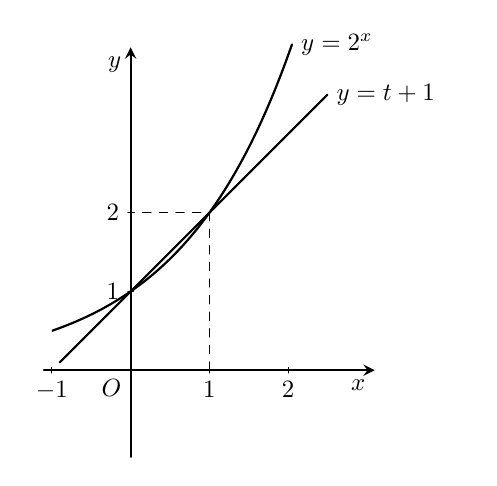
\begin{tikzpicture}[line join=round, line cap=round,>=stealth,thick]
                    \tikzset{every node/.style={scale=0.9}}
                    \draw[->] (-1.1,0)--(3.1,0) node[below left] {$x$};
                    \draw[->] (0,-1.1)--(0,4.1) node[below left] {$y$};
                    \draw (0,0) node [below left] {$O$};
                    \foreach \x in {-1,1,2}
                    \draw[thin] (\x,1pt)--(\x,-1pt) node [below] {$\x$};
                    \foreach \y in {1,2}
                    \draw[thin] (1pt,\y)--(-1pt,\y) node [left] {$\y$};
                    \draw[dashed,thin](1,0)--(1,2)--(0,2);
                    \begin{scope}
                        \clip (-1,-1) rectangle (4.3,4.35);
                        \draw[samples=200,domain=-0.9:2.5,smooth,variable=\x] plot (\x,{1*(\x)+1}) node [right] {$y=t+1$};
                        \draw[samples=200,domain=-1:2.05,smooth,variable=\x] plot (\x,{2^(\x)}) node [right] {$y=2^x$};
                    \end{scope}
                \end{tikzpicture}
            \end{center}
        \end{center}
        Ta có $t=x^2+y^2-2x+1\leq 1\Leftrightarrow(x-1)^2+y^2\leq 1$.\\
        Gọi $(C)$ là đường tròn $(x-1)^2+y^2=1\Rightarrow(C)$ có tâm là $I(1;0)$ và bán kính là $R=1$.\\
        Do đó các cặp số $(x;y)$ thỏa mãn thuộc hình tròn $(C)$.\\
        Lại có $P=\dfrac{4y}{2x+y+1}\Leftrightarrow 2Px+(P-4)y+P=0$ (là PTĐT $\Delta$).\\
        Ta có $\Delta$ và $(C)$ có điểm chung khi $\mathrm{d}(I,\Delta)\leq R\Leftrightarrow\dfrac{\left|2P\cdot 1+(P-4)\cdot 0+P\right|}{\sqrt{4P^2+(P-4)^2}}\leq 1\Leftrightarrow|3P|\leq\sqrt{5P^2-8P+16}\Leftrightarrow 9P^2\leq 5P^2-8P+16\Leftrightarrow P^2+2P-4\leq 0\Leftrightarrow-1-\sqrt{5}\leq P\leq-1+\sqrt{5}$ \\
        $ \Rightarrow M=-1+\sqrt{5};m=-1-\sqrt{5}\Rightarrow M+m=-2 $.
    }
\end{ex}
\begin{ex}%[2D2G3-2]
    [Sở Nghệ An 2022]%Câu 91.
    Cho các số thực $a,b,c>1$ thỏa mãn $6\log_{2ab}c\geq 1+\log_{2b}c$. $\log_ac$ và biết phương trình $c^{x^2+1}=a^x$ có nghiệm. Giá trị lớn nhất của biểu thức $P=\log_a\left(2bc^4\right)$ bằng $\dfrac{m+\sqrt{n}}{p}$ trong đó $m,n,p$ là các số nguyên dương và $\dfrac{m}{p}$ là phân số tối giản. Giá trị của $m+n+p$ bằng
    \choice
    {$48$}
    {$60$}
    {$56$}
    {\True $64$}
    \loigiai{
        Ta có $c^{x^2+1}=a^x\Leftrightarrow x^2+1=x\log_ca\Rightarrow\log_ca=x+\dfrac{1}{x}\geq 2\sqrt{x\cdot\dfrac{1}{x}}=2\Leftrightarrow\dfrac{1}{\log_ca}\leq\dfrac{1}{2}\Rightarrow\log_ca+\dfrac{1}{\log_ca}=\dfrac{5}{2}$ (1). Tiếp đến ta có: $6\log_{2ab}c\geq 1+\log_{2b}c\cdot\log_ac\Leftrightarrow\dfrac{6}{\log_c2b+\log_ca}\geq 1+\dfrac{1}{\log_c2b}\cdot\dfrac{1}{\log_ca}\Leftrightarrow 6\geq\left(1+\dfrac{1}{\log_c2b}\cdot\dfrac{1}{\log_ca}\right)\left(\log_c2b+\log_ca\right)\Leftrightarrow 6\geq\log_c2b+\log_ca+\dfrac{1}{\log_c2b}+\dfrac{1}{\log_ca}$ (1) $\Leftrightarrow\log_c2b+\dfrac{5}{2}+\dfrac{1}{\log_c2b}\leq 6\Leftrightarrow\log_c2b\in\left[\dfrac{7-\sqrt{33}}{4};\dfrac{7+\sqrt{33}}{4}\right]$. Từ đó ta suy ra: $P=\log_a\left(2bc^4\right)=\log_a(2b)+4\log_ac=\dfrac{\log_c(2b)}{\log_ca}+\dfrac{4}{\log_ca}=\dfrac{\log_c(2b)+4}{\log_ca}\leq\dfrac{\dfrac{7+\sqrt{33}}{4}+4}{2}=\dfrac{23+\sqrt{33}}{8}$ Đồng nhất hệ số suy ra $\heva{&m=23;n=33\\&p=8}$ tức $m+n+p=64$.
    }
\end{ex}
\begin{ex}%[2D2G3-2]
    [THPT Thanh Miện 2 - Hải Dương 2022]%Câu 92.
    Cho các số thực $a,b,m,n$ thoả mãn $2m+n<0$ và $\heva{&\log_2\left(a^2+b^2+9\right)=1+\log_2(3a+2b)\\&9^{-m}{\cdot 3}^{-n}{\cdot 3}^{-\frac{4}{2m+n}}+\ln\left[(2m+n+2)^2+1\right]=81}$. Tìm giá trị nhỏ nhất của biểu thức $P=\sqrt{(a-m)^2+(b-n)^2}$.
    \choice
    {$2$}
    {$2\sqrt{5}$}
    {$\sqrt{5}-2$}
    {\True $2\sqrt{5}-2$}
    \loigiai{
        Điều kiện $3a+2b>0$.\\
        Ta có $\log_2\left(a^2+b^2+9\right)=1+\log_2(3a+2b)\Leftrightarrow a^2+b^2+9=6a+4b\Leftrightarrow(a-3)^2+(b-2)^2=4$.\\
        Suy ra $A(a;b)$ thuộc đường tròn $(C)$ tâm $I(3;2)$, bán kính $R=2$.\\
        Ta có $9^{-m}\cdot 3^{-n}\cdot 3^{-\frac{4}{2m+n}}+\ln\left[(2m+n+2)^2+1\right]=81\Leftrightarrow 3^{-2m-n-\dfrac{4}{2m+n}}+\ln\left[(2m+n+2)^2+1\right]=81$.\\
        Mặt khác, $(2m+n+2)^2+1\geq 1$ \\
        $ \Rightarrow\ln\left[(2m+n+2)^2+1\right]\geq 0 $ \\
        $ \Rightarrow 3^{-2m-n-\frac{4}{2m+n}}+\ln\left[(2m+n+2)^2+1\right]\geq 3^{-2m-n+\frac{4}{-2m-n}}\geq 3^{2\cdot\sqrt{(-2m-n)\frac{4}{-2m-n}}}=81 $.\\
        Dấu đẳng thức xảy ra $\Leftrightarrow-2m-n=2\Leftrightarrow 2m+n+2=0$.\\
        Do đó, $B(m;n)$ thuộc đường thẳng $\Delta\colon 2x+y+2=0$.\\
        Ta có $P=AB\geq\mathrm{d}(I,\Delta)-R=2\sqrt{5}-2$.
    }
\end{ex}
\begin{dang}
    {Sử dụng phương pháp hàm số (hàm đặc trưng) giải các bài toán logarit}
\end{dang}
\begin{ex}%[2D2G3-2]
    [THPT Đào Duy Từ - Hà Nội - 2021]%Câu 93.
    Cho các số thực dương $a, b, x, y$ thỏa mãn $a>1, b>1$ và $a^{x-1}=b^y=\sqrt[3]{ab}$. Giá trị nhỏ nhất của biểu thức $P=3x+4y$ thuộc tập hợp nào dưới đây?
    \choice
    {\True $(7;9]$}
    {$(11;13)$}
    {$(1;2)$}
    {$[5;7)$}
    \loigiai{
        $a^{x-1}=b^y=\sqrt[3]{ab}\Rightarrow\heva{&x-1=y\cdot\log_ab\\&y=\dfrac{1}{3}\cdot (1+\log_ba)}\Rightarrow\heva{&\log_ab=\dfrac{x-1}{y}\\&\log_ab=\dfrac{1}{3y-1}}\Rightarrow\dfrac{x-1}{y}=\dfrac{1}{3y-1}\Leftrightarrow x=\dfrac{4y-1}{3y-1.}$ \\
        Vì $a>1, b>1$ nên $\log_ab>0$. Suy ra $y>\dfrac{1}{3}$.\\
        $P=3x+4y=3\cdot\dfrac{4y-1}{3y-1}+4y=\dfrac{12y^2+8y-3}{3y-1}$.\\
        Xét hàm số $f(y)=\dfrac{12y^2+8y-3}{3y-1}; y>\dfrac{1}{3}$.\\
        $f^/(y)=\dfrac{36y^2-24y+1}{(3y-1)^2}=0\Leftrightarrow y=\dfrac{2\pm\sqrt{3}}{6}$.\\
        Bảng biến thiên:
        \begin{center}
            
\begin{tikzpicture}
                \tkzTabInit[espcl=3,lgt=1.5,nocadre]
                {$x$/0.7,$y'$/0.7,$y$/2.1}
                {$\frac{1}{3}$,$\frac{2+\sqrt 3}{6}$,$+\infty$}
                \tkzTabLine{d,-,0,+,}
                \tkzTabVar{D+/$+\infty$,-/$f\left(\frac{2+\sqrt 3}{6}\right)$,+/$+\infty$}
            \end{tikzpicture}
        \end{center}
        Từ bảng biến thiên, suy ra $P_{\min} =f\left(\dfrac{2+\sqrt{3}}{6}\right)\approx 7,64$.
    }
\end{ex}
\begin{ex}%[2D2G3-2]
    [Chuyên Quang Trung - Bình Phước - 2021]%Câu 94.
    Số giá trị $m$ nguyên, $m\in[-20;20]$, sao cho $\min\limits_{x\in[0,3; 1]}\left|\dfrac{\log_{0,3}x^m+16}{\log_{0,3}x+m}\right|=16$ là
    \choice
    {$5$}
    {\True $1$}
    {$20$}
    {$40$}
    \loigiai{
        Đặt $t=\log_{0,3}x$.\\
        Đặt $f(x)=\dfrac{m\log_{0,3}x+16}{\log_{0,3}x+m} (x>0)$.\\
        Khi đó: Xét $f(t)=\dfrac{mt+16}{t+m}$ trên đoạn $[0; 1]$.\\
        Từ đó $f'(t)=\dfrac{m^2-16}{(t+m)^2}$.,\\
        $f(0)=\dfrac{16}{m}$, $f(1)=\dfrac{m+16}{m+1}$ (Điều kiện $m\neq 0,-1$).\\
        Trường hợp 1: $m\in[-20;-4]\Rightarrow f'(t)=\dfrac{m^2-16}{(t+m)^2} >0,\forall t\in[0;1]$.\\
        Nên hàm số đồng biến trên khoảng $(0;1)$.\\
        Suy ra, $f(0)\leq f(t)\leq f(1)<0$ nên $\left|f(0)\right|\geq\left|f(t)\right|\geq\left|f(1)\right|>0$, $\forall t\in[0;1]$.\\
        Nên $\max\limits_{t\in[0;1]} f(t)=f(1)=\dfrac{m+16}{m+1}<0\Rightarrow\min\limits_{t\in[0;1]}\left|f(t)\right|=\left|f(1)\right|=\left|\dfrac{m+16}{m+1}\right|(m\neq-1)$.\\
        Mà $\left|\dfrac{m+16}{m+1}\right|=16\Leftrightarrow\hoac{&m=0(l)\\&m=\dfrac{-32}{17}(l).}$ \\
        Trường hợp 2: $m\in[-4;0]\Rightarrow f'(t)=\dfrac{m^2-16}{(t+m)^2} <0,\forall t\in[0;1]$.\\
        Nên hàm số nghịch biến trên đoạn $[0;1]$.\\
        Suy ra, $0>f(0)\geq f(t)\geq f(1)$ nên $\left|f(1)\right|\geq\left|f(t)\right|\geq\left|f(0)\right|>0$, $\forall t\in[0;1]$.\\
        Nên $\max\limits_{x\in[0;1]} f(x)=f(0)\Rightarrow\min\limits_{x\in[0;1]}\left|f(x)\right|=\left|f(0)\right|=\left|\dfrac{16}{m}\right|(m\neq 0)$.\\
        Mà $\left|\dfrac{16}{m}\right|=16\Leftrightarrow\hoac{&m=1(l)\\&m=-1(l).}$ \\
        Trường hợp 3: $m\in[0;4]\Rightarrow f'(t)=\dfrac{m^2-16}{(t+m)^2} <0,\forall t\in[0;1]$.\\
        Nên hàm số nghịch biến trên khoảng $(0; 1)$.\\
        Suy ra, $f(0)\geq f(t)\geq f(1)>0$ nên $\left|f(1)\right|\geq\left|f(t)\right|\geq\left|f(0)\right|>0$, $\forall t\in[0;1]$.\\
        Nên $\min\limits_{x\in[0;1]} f(t)=f(1)\Rightarrow\min\limits_{x\in[0;1]}\left|f(t)\right|=\left|f(1)\right|=\left|\dfrac{m+16}{m+1}\right|(m\neq-1)$.\\
        Mà $\left|\dfrac{m+16}{m+1}\right|=16\Leftrightarrow\hoac{&m=0(n)\\&m=\dfrac{-32}{17}(l).}$ \\
        Trường hợp 4: $m\in[4;20]\Rightarrow f'(t)=\dfrac{m^2-16}{(t+m)^2} >0,\forall t\in[0;1]$.\\
        Nên hàm số đồng biến trên khoảng $(0;1)$.\\
        Suy ra, $0<f(0)\leq f(t)\leq f(1)$ nên $0<\left|f(0)\right|\leq\left|f(t)\right|\leq\left|f(1)\right|$, $\forall t\in[0;1]$.\\
        Nên $\min\limits_{x\in[0;1]} f(t)=f(0)\Rightarrow\min\limits_{x\in[0;1]}\left|f(t)\right|=\left|f(0)\right|=\left|\dfrac{16}{m}\right|(m\neq 0)$.\\
        Mà $\left|\dfrac{16}{m}\right|=16\Leftrightarrow\hoac{&m=1(l)\\&m=-1(l).}$ \\
        Vậy tổng hợp các trường hợp: $m=1$ thì thỏa ycbt. Chọn $B$.
    }
\end{ex}
\begin{ex}%[2D2G3-2]
    [THPT Quảng Xương 1 - Thanh Hóa - 2021]%Câu 95.
    Gọi $S$ là các cặp số thực $(x, y)$ sao cho $\ln(x-y)^x-2020x=\ln(x-y)^y-2020y+\mathrm{e}^{2021}$ và $x\in[-1; 1]$. Biết rằng giá trị lớn nhất của biểu thức $P=\mathrm{e}^{2021x}(y+1)-2021x^2$ với $(x,y)\in S$ đạt được tại $(x_0; y_0)$. Mệnh đề nào sau đây đúng?
    \choice
    {\True $x_0\in\left[\dfrac{1}{2};1\right]$}
    {$x_0\in\left[\dfrac{1}{4};\dfrac{1}{2}\right]$}
    {$x_0\in[-1;0)$}
    {$x_0\in\left[0;\dfrac{1}{4}\right)$}
    \loigiai{
        Điều kiện $x-y>0$.\\
        Ta có $\ln(x-y)^x-2020x=\ln(x-y)^y-2020y+\mathrm{e}^{2021}$ \\
        $\Leftrightarrow(x-y)\ln(x-y)-2020(x-y)=\mathrm{e}^{2021}\Leftrightarrow\ln(x-y)-2020-\dfrac{\mathrm{e}^{2021}}{x-y}=0(*) $.\\
        Xét hàm $f(t)=\ln t-2020-\dfrac{\mathrm{e}^{2021}}{t}$, có $f'(t)=\dfrac{1}{t}+\dfrac{\mathrm{e}^{2021}}{t}>0,\forall t>0$.\\
        Do đó $f(t)$ đồng biến trên khoảng $(0;+\infty)$.\\
        Suy ra $(*)\Leftrightarrow f(x-y)=0=f\left(\mathrm{e}^{2021}\right)\Leftrightarrow x-y=\mathrm{e}^{2021}\Leftrightarrow y=x-\mathrm{e}^{2021}$.\\
        Khi đó $P=\mathrm{e}^{2021x}\left(1+x-\mathrm{e}^{2021}\right)-2021x^2=g(x)$.\\
        $g'(x)=\mathrm{e}^{2021x}\left(2022+2021x-2021\mathrm{e}^{2021}\right)-4042x$.\\
        $g''(x)=\mathrm{e}^{2021x}\left(2021\cdot 2022+2021^2x-2021^2\mathrm{e}^{2021}\right)-4042$.\\
        $\leq\mathrm{e}^{2021x}\left(2021\cdot 2022+2021^2x-2021^2\mathrm{e}^{2021}\right)-4042<0,\forall x\in[-1; 1]$.\\
        Nên $g'(x)$ nghịch biến trên đoạn $[-1; 1]$.\\
        Mà $g'(-1)=\mathrm{e}^{-2021}+2021>0, g'(0)=2022-2021\mathrm{e}^{2021}<0$ nên tồn tại $x_0\in(-1; 0)$ sao cho $g(x_0)=0$ và khi đó $\max\limits_{[-1; 1]} g(x)=g(x_0)$. Vậy $P$ lớn nhất tại $x_0\in(-1; 0)$.}
\end{ex}
\begin{ex}%[2D2G3-2]
    [Trung Tâm Thanh Tường - 2021]%Câu 96.
    Cho $x,y$ là hai số thực dương thỏa mãn $2x\cdot\log_2\dfrac{x}{y+1}=y-4x+1$. Giá trị lớn nhất của biểu thức $P=x^2-y^2$ là
    \choice
    {$\dfrac{5}{12}$}
    {$\dfrac{7}{12}$}
    {$\dfrac{1}{12}$}
    {\True $\dfrac{2}{3}$}
    \loigiai{
        Đặt $t=\log_2\dfrac{x}{y+1}\Rightarrow y+1=\dfrac{x}{2^t}$.\\
        $2x\cdot\log_2\dfrac{x}{y+1}=y-4x+1$ trở thành: $2x\cdot t=\dfrac{x}{2^t}-4x\Leftrightarrow 2t\cdot 2^t+4\cdot 2^t=1\Leftrightarrow 2^t(t+2)=\dfrac{1}{2}\Leftrightarrow t=-1$ \\
        $\Rightarrow\log_2\dfrac{x}{y+1}=-1\Leftrightarrow\dfrac{x}{y+1}=\dfrac{1}{2}\Leftrightarrow y=2x-1 $ \\
        $ \Rightarrow P=x^2-(2x-1)^2=-3x^2+4x-1\Rightarrow P'(x)=-6x+4=0\Leftrightarrow x=\dfrac{2}{3}\Rightarrow\mathrm{P}\left(\dfrac{2}{3}\right)=\dfrac{1}{3} $.\\
        Bảng biến thiên của $\mathrm{P}(x)$ trên $(0;+\infty)$:
        \begin{center}
            
\begin{tikzpicture}
                \tkzTabInit[nocadre,lgt=1,espcl=3]{$x$/1.0,$P$/2.5}{$0$,$\dfrac{2}{3}$,$+\infty$}
                \tkzTabVar{-/$-1$,+/$\dfrac{1}{3}$,-/$-\infty$}
            \end{tikzpicture}
        \end{center}
        Vậy $P_{\max} =\dfrac{1}{3}$ khi $x=\dfrac{2}{3}$ (Không có trong các phương án đưa ra).
    }
\end{ex}
\begin{ex}%[2D2G3-2]
    [Chuyên AMSTERDAM - Hà Nội - 2021]%Câu 97.
    Cho $x,y>0$ là các số thực dương thỏa mãn $\log_{2021}x+\log_{2021}y\geq\log_{2021}\left(x^2+y\right)$. Gọi $T_{\min}$ là giá.\\
    trị nhỏ nhất của biểu thức $T=3x+y$. Mệnh đề nào dưới đây đúng?
    \choice
    {$T_{\min}\in(13;15)$}
    {$T_{\min}\in(10;12)$}
    {\True $T_{\min}\in(8;10)$}
    {$T_{\min}\in(15;17)$}
    \loigiai{
        Ta có $\log_{2021}x+\log_{2021}y\geq\log_{2021}\left(x^2+y\right)$ \\
        $\Leftrightarrow\log_{2021}xy\geq\log_{2021}\left(x^2+y\right) $ \\
        $ \Leftrightarrow xy\geq x^2+y\Leftrightarrow y(x-1)\geq x^2 $ (1).\\
        Do $x,y>0$ nên từ (1) suy ra $x>1$. Khi đó từ (1) ta cũng có $y\geq\dfrac{x^2}{x-1}$.\\
        Ta có $T=3x+y\geq 3x+\dfrac{x^2}{x-1}=\dfrac{4x^2-3x}{x-1}$.\\
        Xét hàm $g(x)=\dfrac{4x^2-3x}{x-1}$ với $x\in(1;+\infty)$.\\
        Có $g'(x)=\dfrac{4x^2-8x+3}{(x-1)^2}$.\\
        $g'(x)=0\Leftrightarrow\hoac{&x=\dfrac{3}{2}\in(1;+\infty)\\&x=\dfrac{1}{2}\notin(1;+\infty).}$ \\
        Bảng biến thiên của hàm $g(x)=\dfrac{4x^2-3x}{x-1}$ như sau:
        \begin{center}
            
\begin{tikzpicture}
                \tkzTabInit[nocadre,lgt=1.2,espcl=3]{$x$/1,$g'(x)$/0.8,$g(x)$/2}{$1$,$\dfrac{3}{2}$,$+\infty$}
                \tkzTabLine{,-,0,+,}
                \tkzTabVar{+/$+\infty$,-/$9$,+/$+\infty$}
            \end{tikzpicture}
        \end{center}
        Từ bảng biến thiên suy ra $\min\limits_{(1;+\infty)} g(x)=9\Leftrightarrow x=\dfrac{3}{2}$. Vậy $T_{\min} =9$ khi $x=\dfrac{3}{2}$, $y=\dfrac{9}{2}$.
    }
\end{ex}
\begin{ex}%[2D2G3-2]
    [Chuyên Quốc Học Huế - 2021]%Câu 98.
    Gọi $S$ là tập hợp các cặp số thực $(x; y)$ thỏa mãn đẳng đẳng thức sau đây.\\
    $2^{2x-y+1}+2^{-2x+y+1}+3^{2x-y+1}+3^{-2x+y+1}=5^{^{2x-y+1}}+5^{-2x+y+1}$.\\
    Biết rằng giá trị nhỏ nhất của biểu thức $P=y^2+2021x-3$ với $(x; y)\in S$ đạt được tại $(x_0; y_0)$.\\
    Khẳng định nào sau đây đúng?
    \choice
    {$x_0\in(0; 100)$}
    {$x_0\in(-200;-100)$}
    {$x_0\in(-100; 0)$}
    {\True $x_0\in(-300;-200)$}
    \loigiai{
        Đặt $t=2x-y$, ta được: $2^{t+1}+2^{1-t}+3^{t+1}+3^{1-t}-\left(5^{t+1}+5^{1-t}\right)=0$.\\
        Xét hàm $f(t)=2^{t+1}+2^{1-t}+3^{t+1}+3^{1-t}-\left(5^{t+1}+5^{1-t}\right)$ với $t\in\mathbb{R}$.\\
        $f'(t)=\left(2^{t+1}-2^{1-t}\right)\ln 2+\left(3^{t+1}-3^{1-t}\right)\ln 3-\left(5^{t+1}-5^{1-t}\right)\ln 5$.\\
        $f''(t)=\left(2^{t+1}+2^{1-t}\right)\ln^22+\left(3^{t+1}+3^{1-t}\right)\ln^23-\left(5^{t+1}+5^{1-t}\right)\ln^25$.\\
        Xét hàm $h(u)=u^{t+1}+u^{1-t}$ (với $t$: hằng số; $u>1$).\\
        $h'(u)=(t+1)u^t+(1-t)u^{-t}=t\left(u^t-u^{-t}\right)+u^t+u^{-t} =\dfrac{t\left(u^{2t}-1\right)}{u^t}+u^t+u^{-t}$.\\
        Ta thấy nếu:\\
        $t\geq 0$ thì $u^{2t}-1\geq 0$.\\
        $t<0$ thì $u^{2t}-1<0$.\\
        Và $u^t+u^{-t}>0;$.\\
        Nên $h'(u)=\dfrac{t\left(u^{2t}-1\right)}{u^t}+u^t+u^{-t}>0;\forall u>1$.\\
        Suy ra: $h(u)$ đồng biến trên $(1;+\infty)$.\\
        $h(2)<h(5); h(3)<h(5)$.\\
        $f''(t)=h(2)\ln^22+h(3)\ln^23-h(5)\ln^25<h(5)\left[\ln^22+\ln^23-\ln^25\right]<0$.\\
        Từ đó $f'(t)$ nghịch biến trên $\mathbb{R}$. Mà $f'(0)=0$ nên ta có bảng biến thiên:
        \begin{center}
            
\begin{tikzpicture}
                \tkzTabInit[nocadre,lgt=1.2,espcl=3]{$t$/0.8,$f'(t)$/0.8,$f(t)$/2}{$-\infty$,$0$,$+\infty$}
                \tkzTabLine{,+,0,-,}
                \tkzTabVar{-/{},+/$0$,-/{}}
            \end{tikzpicture}
        \end{center}
        $f(0)=0\Leftrightarrow 2x-y=0\Leftrightarrow y=2x$.\\
        Theo đề bài ta có:\\
        $P=y^2+2021x-3=4x^2+2021x-3$ đạt GTNN khi và chỉ khi $x=-\dfrac{2021}{8}$.\\
        Vậy $x\in(-300;-200)$.
    }
\end{ex}
\begin{ex}%[2D2G3-2]
    [Sở Quảng Bình - 2021]%Câu 99.
    Cho các số thực dương $x, y$ thỏa mãn $\mathrm{e}^{x+y}\leq \mathrm{e}(x+y)$. Giá trị nhỏ nhất của biểu thức $P=\dfrac{1}{x^3+y^3}-\dfrac{1}{x+y}-2020$ bằng
    \choice
    {\True $2\sqrt{3}-2016$}
    {$-2012$}
    {$2\sqrt{3}-2020$}
    {$2-\sqrt{3}$}
    \loigiai{
        Xét hàm số $f(t)=\mathrm{e}^t-\mathrm{e}t$ với $t>0$. Ta có $f'(t)=\mathrm{e}^t-\mathrm{e}$, $f'(t)=0\Leftrightarrow t=1$.\\
        BBT
        \begin{center}
            
\begin{tikzpicture}
                \tkzTabInit[nocadre,lgt=1.2,espcl=3]{$t$/0.8,$f'(t)$/0.8,$f(t)$/2.5}{$0$,$1$,$+\infty$}
                \tkzTabLine{,-,0,+,}
                \tkzTabVar{+/$1$,-/$0$,+/$+\infty$}
            \end{tikzpicture}
        \end{center}
        Từ BBT ta có $f(t)\geq 0\forall t>0$ và $f(t)=0\Leftrightarrow t=1$.\\
        Từ giả thiết ta có $f(x+y)\leq 0$. Vậy $f(x+y)=0\Leftrightarrow x+y=1$.\\
        Ta có $P=\dfrac{1}{x^3+y^3}+\dfrac{1}{xy}-2020=\dfrac{1}(x+y)\left[(x+y)^2-3xy\right]+\dfrac{1}{xy}-2020=\dfrac{1}{1-3xy}+\dfrac{1}{xy}-2020$.\\
        Đặt $u=xy$ thì $0<u\leq\left(\dfrac{x+y}{2}\right)^2=\dfrac{1}{4}$.\\
        Xét hàm số $g(u)=\dfrac{1}{1-3u}+\dfrac{1}{u}$ với $0<u\leq\dfrac{1}{4}$.\\
        Có $g'(u)=\dfrac{3}{(1-3u)^2}-\dfrac{1}{u^2}$, $g'(u)=0\Leftrightarrow u=\dfrac{3-\sqrt{3}}{6}$.\\
        Bảng biến thiên
        \begin{center}
            
\begin{tikzpicture}
                \tkzTabInit[nocadre,lgt=1.2,espcl=3]{$u$/1.0,$g'(u)$/0.8,$g(u)$/2.5}{$0$,$\dfrac{3-\sqrt{3}}{6}$,$\dfrac{1}{4}$}
                \tkzTabLine{,-,0,+,}
                \tkzTabVar{+/$1$,-/$4+2\sqrt{3}$,+/$8$}
            \end{tikzpicture}
        \end{center}
        Vậy $\min\limits_{u\in\left(0;\frac{1}{4}\right]}g(u)=4+2\sqrt{3}$ nên $\min P=2\sqrt{3}-2016$.
    }
\end{ex}
\begin{ex}%[2D2G3-2]
    [Chuyên Lê Thánh Tông 2019]%Câu 100.
    Cho hai số thực dương $x, y$ thỏa mãn $2^{\ln\left(\frac{x+y}{2}\right)}\cdot 5^{\ln(x+y)}=2^{\ln 5}$. Tìm giá trị lớn nhất của biểu thức $P=(x+1)\ln x+(y+1)\ln y$.
    \choice
    {$P_{\max} =10$}
    {\True $P_{\max} =0$}
    {$P_{\max} =1$}
    {$P_{\max} =\ln 2$}
    \loigiai{
        $2^{\ln\left(\frac{x+y}{2}\right)}\cdot 5^{\ln (x+y)}=2^{\ln 5}\Leftrightarrow 2^{\ln (x+y)-\ln 2}\cdot 5^{\ln (x+y)}=2^{\ln 5}\Leftrightarrow 2^{\ln (x+y)}\cdot 5^{\ln (x+y)}=2^{\ln 5}\cdot 2^{\ln 2}\Leftrightarrow 10^{\ln (x+y)}=2^{\ln 10}$ \\
        $ \Leftrightarrow\ln (x+y)=\log\left(2^{\ln 10}\right)\Leftrightarrow\ln (x+y)=\ln 10\cdot\log 2\Leftrightarrow\mathrm{e}^{\ln (x+y)}=\mathrm{e}^{\ln 10\cdot\log 2}\Leftrightarrow x+y=10^{\log 2}\Leftrightarrow x+y=2 $.\\
        Do đó $P=(x+1)\ln x+(3-x)\ln(2-x)$.\\
        Xét hàm số $f(x)=(x+1)\ln x+(3-x)\ln (2-x)$.\\
        $f'(x)=\ln x+\dfrac{x+1}{x}-\ln (2-x)-\dfrac{3-x}{2-x}=\ln\dfrac{x}{2-x}+\dfrac{2-2x}{x(2-x)}$.\\
        $f''(x)=-\dfrac{1}{(2-x)^2}\cdot\dfrac{2-x}{x}-\dfrac{2x^2-4x+4}{\left(2x-x^2\right)^2}<0,\forall x\in(0;2)$.\\
        Do đó $f'(x)=0$ có nhiều nhất một nghiệm trên $(0;2)$.\\
        Mà $x=1$ là một nghiệm của pt $f'(x)=0$ nên phương trình $f'(x)=0$ có nghiệm duy nhất là $x=1$.\\
        Lập bảng biến thiên ta được $\max f(x)=f(1)=0$.
    }
\end{ex}
\begin{ex}%[2D2G3-2]
    [Chuyên Hạ Long 2019]%Câu 101.
    Cho các số thực $a,b$ thỏa mãn $a\geq b>1$. Biết rằng biểu thức $P=\dfrac{1}{\log_{ab}a}+\sqrt{\log_a\dfrac{a}{b}}$ đạt giá trị lớn nhất khi $b=a^k$. Khẳng định nào sau đây là sai
    \choice
    {\True $k\in[2;3]$}
    {$k\in(0;1)$}
    {$k\in[0;1]$}
    {$k\in\left(0;\dfrac{3}{2}\right)$}
    \loigiai{
        Ta có $a\geq b>1\Rightarrow\log_ab>0$.\\
        $P=\dfrac{1}{\log_{ab}a}+\sqrt{\log_a\dfrac{a}{b}}=\log_aab+\sqrt{\log_aa-\log_ab}=1+\log_ab+\sqrt{1-\log_ab}$.\\
        Đặt $t=\sqrt{1-\log_ab}(t\geq 0)\Rightarrow\log_ab=1-t^2$. Ta có $P=-t^2+t+2$ trên $[0;+\infty)$.\\
        Bảng biến thiên.\\
        \begin{center}
            
\begin{tikzpicture}
                \tkzTabInit[espcl=2.5,lgt=1.5,nocadre]
                {$x$/0.7,$y'$/0.7,$y$/2.1}
                {$-\infty$,$\frac{1}{2}$,$+\infty$}
                \tkzTabLine{,+,0,-,}
                \tkzTabVar{-/$-\infty$,+/$\frac{9}{4}$,-/$-\infty$}
            \end{tikzpicture}
        \end{center}
        Hàm số đạt giá trị lớn nhất tại $t=\dfrac{1}{2}$.\\
        Với $t=\dfrac{1}{2}\Rightarrow\dfrac{1}{2}=\sqrt{1-\log_ab}\Leftrightarrow\log_ab=\dfrac{3}{4}\Leftrightarrow b=a^{\frac{3}{4}}\Rightarrow k=\dfrac{3}{4}$.
    }
\end{ex}
\begin{ex}%[2D2G3-2]
    [Chuyên Vĩnh Phúc 2019]%Câu 102.
    Cho $a$, $b$ là các số dương thỏa mãn $b>1$ và $\sqrt{a}\leq b<a$. Tìm giá trị nhỏ nhất của biểu thức $P=\log_{\frac{a}{b}}a+2\log_{\sqrt{b}}\left(\dfrac{a}{b}\right)$.
    \choice
    {$6$}
    {$7$}
    {$5$}
    {\True $4$}
    \loigiai{
        Ta có $P=\dfrac{1}{1-\log_ab}+4\cdot (log_ba-1)=\dfrac{1}{1-\dfrac{1}{\log_ba}}+4\cdot (log_ba-1)$.\\
        Đặt $t=\log_ba$. Vì $\sqrt{a}\leq b<a\Rightarrow\log_b(\sqrt{a})\leq 1\leq\log_ba\Leftrightarrow\dfrac{t}{2}<1<t\Leftrightarrow 1<t<2$ \\
        $\Rightarrow P=\dfrac{1}{1-\dfrac{1}{t}}+4(t-1)=\dfrac{t}{t-1}+4(t-1) $ với $t\in(1;2)$.\\
        Xét hàm số $f(t)=\dfrac{t}{t-1}+4(t-1)$ với $t\in(1;2)$.\\
        $f'(t)=\dfrac{-1}{(t-1)^2}+4, f'(t)=0\Leftrightarrow(t-1)^2=\dfrac{1}{4}\Leftrightarrow\hoac{&t=\dfrac{3}{2}(tm)\\&t=\dfrac{1}{2}(l).}$ \\
        Bảng biến thiên
        \begin{center}
            
\begin{tikzpicture}
                \tkzTabInit[espcl=2.5,lgt=1.5,nocadre]
                {$x$/0.7,$y'$/0.7,$y$/2.1}
                {$1$,$\frac{3}{2}$,$2$}
                \tkzTabLine{,-,0,+,}
                \tkzTabVar{+/$+\infty$,-/$5$,+/$6$}
            \end{tikzpicture}
        \end{center}
        Từ bảng biến thiên suy ra: $\min\limits_{(1;2)} f(t)=f\left(\dfrac{3}{2}\right)=5$.\\
        Vậy giá trị nhỏ nhất của biểu thức $P$ bằng $5$.
    }
\end{ex}
\begin{ex}%[2D2G3-2]
    [Chuyên Vĩnh Phúc 2019]%Câu 103.
    Xét các số thực dương $x$, $y$ thỏa mãn $\log_{\frac{1}{2}}x+\log_{\frac{1}{2}}y\leq\log_{\frac{1}{2}}\left(x+y^2\right)$. Tìm giá trị nhỏ nhất $P_{\min}$ của biểu thức $P=x+3y$.
    \choice
    {\True $P_{\min} =9$}
    {$P_{\min} =8$}
    {$P_{\min} =\dfrac{25\sqrt{2}}{4}$}
    {$P_{\min} =\dfrac{17}{2}$}
    \loigiai{
        Ta có\\
        $\log_{\frac{1}{2}}x+\log_{\frac{1}{2}}y\leq\log_{\frac{1}{2}}\left(x+y^2\right)\Leftrightarrow\log_{\frac{1}{2}}(xy)\leq\log_{\frac{1}{2}}\left(x+y^2\right)\Leftrightarrow xy\geq x+y^2$\\
        $ \Leftrightarrow x(y-1)\geq y^2\Leftrightarrow\heva{&x\geq\dfrac{y^2}{y-1}\\&y>1}$ (Vì $x;y>0$).\\
        Ta có $P=x+3y\geq\dfrac{y^2}{y-1}+3y=4y+1+\dfrac{1}{y-1}$.\\
        Xét hàm số: $f(y)=4y+1+\dfrac{1}{y-1};y>1$.\\
        Đạo hàm: $f^/(y)=4-\dfrac{1}{(y-1)^2}$.\\
        $f^/(y)=0\Leftrightarrow\hoac{&y=\dfrac{3}{2}(n)\\&y=\dfrac{1}{2}(l).}$ \\
        Bảng biến thiên.
        \begin{center}
            
\begin{tikzpicture}
                \tkzTabInit[nocadre,lgt=1.2,espcl=3]{$y$/1.0,$f'(y)$/0.8,$f(y)$/2}{$1$,$\dfrac{3}{2}$,$+\infty$}
                \tkzTabLine{,-,0,+,}
                \tkzTabVar{+/$+\infty$,-/$9$,+/$+\infty$}
            \end{tikzpicture}
        \end{center}
    }
\end{ex}
\begin{ex}%[2D2G3-2]
    [Chuyên Vĩnh Phúc 2019]%Câu 104.
    Cho $x,y$ là các số thực dương thỏa mãn $\log_{2019}x+\log_{2019}y\geq\log_{2019}\left(x^2+y\right)$. Gọi $T_{\min}$ là giá trị nhỏ nhất của biểu thức $T=2x+y$. Mệnh đề nào dưới đây đúng?
    \choice
    {\True $T_{\min}\in(7;8)$}
    {$T_{\min}\in(6;7)$}
    {$T_{\min}\in(5;6)$}
    {$T_{\min}\in(8;9)$}
    \loigiai{
        Ta có\\
        $\log_{2019}x+\log_{2019}y\geq\log_{2019}\left(x^2+y\right)\Leftrightarrow\log_{2019}xy\geq\log_{2019}\left(x^2+y\right)\Leftrightarrow xy\geq x^2+y$ \\
        $ \Leftrightarrow y(x-1)\geq x^2\Leftrightarrow\heva{&y\geq\dfrac{x^2}{x-1}\\&x>1.} $ \\
        Ta có $T=2x+y\geq 2x+\dfrac{x^2}{x-1}=3x+1+\dfrac{1}{x-1}$.\\
        Xét hàm số: $f(x)=3x+1+\dfrac{1}{x-1};x>1$.\\
        Đạo hàm: $f^/(x)=3-\dfrac{1}{(x-1)^2}$.\\
        $f^/(x)=0\Leftrightarrow x=1+\dfrac{\sqrt{3}}{3}(do x>1)$.\\
        Bảng biến thiên.
        \begin{center}
            
\begin{tikzpicture}
                \tkzTabInit[nocadre,lgt=1.2,espcl=3]{$x$/1.0,$f'(x)$/0.8,$f(x)$/2}{$1$,$1+\dfrac{\sqrt{3}}{3}$,$+\infty$}
                \tkzTabLine{,-,0,+,}
                \tkzTabVar{+/$+\infty$,-/$4+2\sqrt{3}$,+/$+\infty$}
            \end{tikzpicture}
        \end{center}
        Do đó: $T_{\min} =4+2\sqrt{3}$.
    }
\end{ex}
\begin{ex}%[2D2G3-2]
    [Chuyên Hùng Vương - Gia Lai - 2020]%Câu 105.
    Xét các số thực dương $a,b,x,y$ thỏa mãn $a>1, b>1$ và $a^{x^2}=b^{y^2}=(ab)^2$. Giá trị nhỏ nhất của biểu thức $P=2\sqrt{2}x+y$ thuộc tập hợp nào dưới đây?
    \choice
    {$[10;15)$}
    {\True $[6;10)$}
    {$(1;4)$}
    {$[4;6)$}
    \loigiai{
        Ta có $a^{x^2}=(ab)^2\Rightarrow x^2=\log_a(ab)^2=2(1+\log_ab)\Rightarrow x=\sqrt{2+2\log_ab}$.\\
        $b^{y^2}=(ab)^2\Rightarrow y^2=\log_b(ab)^2=2(1+\log_ba)\Rightarrow y=\sqrt{2+2\log_ba}$.\\
        $P=2\sqrt{2}x+y=4\sqrt{1+\log_ab}+\sqrt{2+2\log_ba}$.\\
        Đặt $t=\log_ab(t>0)$ ta được: $P=4\sqrt{1+t}+\sqrt{2+\dfrac{2}{t}}$.\\
        Xét hàm số $f(t)=4\sqrt{1+t}+\sqrt{2+\dfrac{2}{t}}$, với $t\in(0;+\infty)$.\\
        $f'(t)=\dfrac{2}{\sqrt{1+t}}-\dfrac{1}{t^2\sqrt{2+\dfrac{2}{t}}}; f'(t)=0\Leftrightarrow\dfrac{2}{\sqrt{1+t}}-\dfrac{1}{t^2\sqrt{2+\dfrac{2}{t}}}=0\Leftrightarrow 2t^2\sqrt{2+\dfrac{2}{t}}=\sqrt{1+t}$ \\
        $ \Leftrightarrow 4t^4\left(2+\dfrac{2}{t}\right)=1+t\Leftrightarrow 8t^4+8t^3-t-1=0\Leftrightarrow t=\dfrac{1}{2} $.\\
        Bảng biến thiên của hàm số $f(t)$.
        \begin{center}
            
\begin{tikzpicture}
                \tkzTabInit[nocadre,lgt=1.2,espcl=3]{$t$/1.0,$f'(t)$/0.8,$f(t)$/2}{$0$,$\dfrac{1}{2}$,{}}
                \tkzTabLine{,-,0,+,}
                \tkzTabVar{+/{},-/$3\sqrt{6}$,+/{}}
            \end{tikzpicture}
        \end{center}
        Từ bảng biến thiên suy ra $MinP=\min\limits_{(0;+\infty)} f(t)=3\sqrt{6}\in[6;10)$ khi $\heva{&\log_ab=\dfrac{1}{2}\\&x=\sqrt{3}\\&y=\sqrt{6}}\Leftrightarrow\heva{&a=b^2\\&x=\sqrt{3}\\&y=\sqrt{6}}$.
    }
\end{ex}
\begin{ex}%[2D2G3-2]
    [Chuyên Lào Cai - 2020]%Câu 106.
    Xét các số thực dương $x$, $y$ thỏa mãn $\log_{\pi}x+\log_{\pi}y\geq\log_{\pi}\left(x+y^2\right)$. Biểu thức $P=x+8y$ đạt giá trị nhỏ nhất của bằng
    \choice
    {\True $P_{\min} =16$}
    {$P_{\min} =\dfrac{33}{2}$}
    {$P_{\min} =11\sqrt{2}$}
    {$P_{\min} =\dfrac{31}{2}$}
    \loigiai{
        Từ đề bài $xy\geq x+y^2$ \\
        $ \Leftrightarrow x(y-1)\geq y^2\Leftrightarrow\heva{&x\geq\dfrac{y^2}{y-1}\\&y>1} $ (Vì $x;y>0$).\\
        Ta có $P=x+8y\geq\dfrac{y^2}{y-1}+8y=9y+1+\dfrac{1}{y-1}$.\\
        Xét hàm số: $f(y)=9y+1+\dfrac{1}{y-1};y>1$.\\
        Đạo hàm: $f^/(y)=9-\dfrac{1}{(y-1)^2}$.\\
        $f^/(y)=0\Leftrightarrow\hoac{&y=\dfrac{4}{3}\\&y=\dfrac{2}{3}(l).}$ \\
        Bảng biến thiên, ta thấy giá trị nhỏ nhất của $f(y)$ là $f\left(\dfrac{4}{3}\right)=16$.\\
        Vậy $P_{\min} =16$ khi $x=\dfrac{16}{3}$.
    }
\end{ex}
\begin{ex}%[2D2G3-2]
    [Sở Bình Phước - 2020]%Câu 107.
    Cho $x,y$ là các số thực dương thỏa mãn $\log_2x+\log_2y+1\geq\log_2\left(x^2+2y\right)$. Giá trị nhỏ nhất của biểu thức $x+2y$ bằng
    \choice
    {\True $2\sqrt{2}+3$}
    {$2+3\sqrt{2}$}
    {$3+\sqrt{3}$}
    {$9$}
    \loigiai{
        Với $x>0;y>0$. Ta có:\\
        $\begin{aligned}&\log_2x+\log_2y+1\geq\log_2\left(x^2+2y\right)(1)\\&\Leftrightarrow 2xy\geq x^2+2y(2)\\&\Leftrightarrow 2y(x-1)\geq x^2\\&\Leftrightarrow x-1\geq\dfrac{x^2}{2y}>0\\&\Rightarrow x>1.\end{aligned}$\\
        Đặt $m=x+2y$ ta có:\\
        $\begin{aligned}&(2)\Leftrightarrow x(m-x)\geq x^2-x+m\\&\Leftrightarrow m(x-1)\geq 2x^2-x\\&\Leftrightarrow m\geq\dfrac{2x^2-x}{x-1}.\end{aligned}$\\
        Xét hàm số $g(x)=\dfrac{2x^2-x}{x-1}$ với $x>1$.\\
        Ta tìm thấy $\min\limits_{(1;+\infty)} g(x)=3+2\sqrt{2}$ khi $x=\dfrac{2+\sqrt{2}}{2}$.\\
        Vậy $m\geq 3+2\sqrt{2}$, dấu bằng xảy ra khi $\heva{&x=\dfrac{2+\sqrt{2}}{2}\\&y=\dfrac{4+3\sqrt{2}}{4}}$ (thỏa mãn điều kiện bài toán).\\
        Vậy GTNN của $x+2y$ là $3+2\sqrt{2}$.
    }
\end{ex}
\begin{ex}%[2D2G3-2]
    [Bỉm Sơn - Thanh Hóa - 2020]%Câu 108.
    Xét các số thực dương $x.y$ thỏa mãn $\log_{\frac{1}{2}}x+\log_{\frac{1}{2}}y\leq\log_{\frac{1}{2}}\left(x+y^2\right)$. Tìm giá trị nhỏ nhất $P_{\min}$ của biểu thức $P=x+3y$.
    \choice
    {$P_{\min} =\dfrac{17}{2}$}
    {$P_{\min} =8$}
    {\True $P_{\min} =9$}
    {$P_{\min} =\dfrac{25\sqrt{2}}{4}$}
    \loigiai{
        Ta có $\log_{\frac{1}{2}}x+\log_{\frac{1}{2}}y\leq\log_{\frac{1}{2}}\left(x+y^2\right)\Leftrightarrow\log_{\frac{1}{2}}(xy)\leq\log_{\frac{1}{2}}\left(x+y^2\right)\Leftrightarrow xy\geq x+y^2$ \\
        $ \Leftrightarrow(y-1)x\geq y^2 $.\\
        Do $y>0\Rightarrow y^2>0\Rightarrow(y-1)x\geq y^2>0$. Mà $x>0$ nên $y-1>0$, hay $y>1$.\\
        Khi đó ta có $x\geq\dfrac{y^2}{y-1}$. Suy ra $P=x+3y\geq\dfrac{y^2}{y-1}+3y$.\\
        Xét hàm số $f(y)=\dfrac{y^2}{y-1}+3y$ trên $(1;+\infty)$.\\
        Ta có $f'(y)=\dfrac{y^2-2y}{(y-1)^2}+3 =\dfrac{4y^2-8y+3}{(y-1)^2}$; $f'(y)=0\Leftrightarrow\hoac{&y=\dfrac{1}{2}\notin(1;+\infty)\\&y=\dfrac{3}{2}\in(1;+\infty).}$ \\
        Bảng biến thiên:\\
        \begin{center}
            
\begin{tikzpicture}
                \tkzTabInit[espcl=3,lgt=1.5,nocadre]
                {$x$/0.7,$y'$/0.7,$y$/2.1}
                {$1$,$\frac{3}{2}$,$+\infty$}
                \tkzTabLine{d,-,0,+,}
                \tkzTabVar{D+/$+\infty$,-/$9$,+/$+\infty$}
            \end{tikzpicture}
        \end{center}
        Từ bảng biến thiên suy ra $f(y)\geq f\left(\dfrac{3}{2}\right)=9$. Vậy $P\geq f(y)\geq 9$.\\
        Dấu xảy ra khi và chỉ khi $\heva{&y=\dfrac{3}{2}\\&x=\dfrac{y^2}{y-1}=\dfrac{9}{2}}$.
    }
\end{ex}
\begin{ex}%[2D2G3-2]
    [Lương Thế Vinh - Hà Nội - 2020]%Câu 109.
    Cho các số thực $x,y$ thỏa mãn $\ln y\geq\ln (x^3+2)-\ln 3$. Tìm giá trị nhỏ nhất của biểu thức $H=\mathrm{e}^{4y-x^3-x-2}-\dfrac{x^2+y^2}{2}+x(y+1)-y$.
    \choice
    {\True $1$}
    {$0$}
    {$e$}
    {$\dfrac{1}{e}$}
    \loigiai{
        Do $\ln y\geq\ln\left(x^3+2\right)-\ln 3\Leftrightarrow x^3+2\leq 3y\Leftrightarrow 4y-x^3-x-2\geq y-x$ \\
        $ \Rightarrow H\geq\mathrm{e}^{y-x}-(y-x)-\dfrac{(y-x)^2}{2} $.\\
        Đặt $t=y-x\Rightarrow t\geq\dfrac{x^3+2}{3}-x=\dfrac{x^3-3x+2}{3}=g(x)$ với $x\geq\sqrt[3]{-2}$.\\
        $g'(x)=\dfrac{3x^2-3}{3}$, $g'(x)=0\Leftrightarrow x=\pm 1\Rightarrow g(x)\geq g(1)=0$, suy ra $t\geq 0$.\\
        Xét hàm số $f(t)=\mathrm{e}^t-t-\dfrac{t^2}{2}$ với $t\geq 0$.\\
        $f'(t)=\mathrm{e}^t-1-t$.\\
        $f''(t)=\mathrm{e}^t-1$.\\
        $f''(t)=0\Leftrightarrow e=0$.\\
        Ta có bảng biến thiên như sau\\
        \begin{center}
            \begin{tikzpicture}[line join=round, line cap=round,>=stealth,thick]
                \coordinate (A) at (0,1);
                \coordinate (A') at ($(A) + (0,-6)$);
                \coordinate (B) at (-2,0);
                \coordinate (B') at ($(B) + (8,0)$);
                \coordinate (C) at (-2,-1);
                \coordinate (C') at ($(C) + (8,0)$);
                \coordinate (D) at (-2,-3);
                \coordinate (D') at ($(D) + (8,0)$);
                \draw(A)--(A') (B)--(B') (C)--(C') (D)--(D');
                \node at (-1,0.5) {$t$};
                \node at (-1,-0.5) {$f''(t)$};
                \node at (-1,-2) {$f'(t)$};
                \node at (-1,-4) {$f(t)$};

                \node at (0.3,0.5) {$0$};
                \node at (0.3,-0.5) {$0$};
                \node at (0.3,-2.7) {$0$};
                \node at (0.4,-4.7) {$f(0)$};

                \node at (2.5,-0.5) {$+$};
                \node at (2.5,-2) {$+$};

                \node at (5.5,0.5) {$+\infty$};
                \node at (5.5,-1.3) {$+\infty$};

                \draw[->] (0.5,-2.7)--(5.3,-1.4);
                \draw[->] (1,-4.7)--(5.5,-3.4);
            \end{tikzpicture}
        \end{center}
        Suy ra $H\geq f(0)$.\\
        Vậy $\min H=1$.
    }
\end{ex}
\begin{ex}%[2D2G3-2]
    [Chuyên Sư Phạm Hà Nội - 2020]%Câu 110.
    Cho các số thực $x,y$ thay đổi, thỏa mãn $x>y>0$ và $\ln(x-y)+\dfrac{1}{2}\ln(xy)=\ln(x+y)$. Giá trị nhỏ nhất của $M=x+y$ là
    \choice
    {$2\sqrt{2}$}
    {$2$}
    {\True $4$}
    {$16$}
    \loigiai{
        Với $x>y>0$, ta có $\ln(x-y)+\dfrac{1}{2}\ln(xy)=\ln(x+y)\Leftrightarrow\dfrac{1}{2}\ln(xy)=\ln(x+y)-\ln(x-y)\Leftrightarrow\ln(xy)=2\ln\dfrac{x+y}{x-y}\Leftrightarrow\ln(xy)=\ln\left(\dfrac{x+y}{x-y}\right)^2\Leftrightarrow xy=\left(\dfrac{x+y}{x-y}\right)^2\Leftrightarrow(x-y)^2xy=(x+y)^2$ (*).\\
        Đặt $\heva{&u=x+y>0\\&v=xy>0.}$ \\
        Ta có (*) $\Leftrightarrow\left(u^2-4v\right)v=u^2\Leftrightarrow(v-1)u^2=4v^2\Leftrightarrow u^2=\dfrac{4v^2}{v-1}=f(v)$, $(v>1)$.\\
        $f'(v)=\dfrac{8v(v-1)-4v^2}{(v-1)^2}=\dfrac{4v(v-2)}{(v-1)^2}$, $f'(v)=0\Leftrightarrow v=2$ do $v>1$.\\
        Bảng biến thiên:
        \begin{center}
            
\begin{tikzpicture}
                \tkzTabInit[nocadre,lgt=1.2,espcl=3]{$v$/0.8,$f'(v)$/0.8,$f(v)$/2}{$1$,$2$,$+\infty$}
                \tkzTabLine{,-,0,+,}
                \tkzTabVar{+/$+\infty$,-/$16$,+/$+\infty$}
            \end{tikzpicture}
        \end{center}
        Vậy $\min (x+y)=\min u=4\Leftrightarrow\heva{&x+y=4\\&xy=2\\&x>y>0}\Leftrightarrow\heva{&x=2+\sqrt{2}\\&y=2-\sqrt{2}}$.
    }
\end{ex}
\begin{ex}%[2D2G3-2]
    [Chuyên Lương Văn Chánh - Phú Yên - 2020]%Câu 111.
    Xét các số thực $a, b, x$ thoả mãn $a>1, b>1, 0<x\neq 1$ và $a^{\log_b^x}=b^{\log_a(x^2)}$. Tìm giá trị nhỏ nhất của biểu thức $P=\ln^2a+\ln^2b-\ln (ab)$.
    \choice
    {$\dfrac{1-3\sqrt{3}}{4}$}
    {$\dfrac{e}{2}$}
    {$\dfrac{1}{4}$}
    {\True $-\dfrac{3+2\sqrt{2}}{12}$}
    \loigiai{
        Ta có $a^{\log_b^x}=b^{\log_a(x^2)}\Leftrightarrow\ln\left(a^{\log_b^x}\right)=\ln\left(b^{\log_a(x^2)}\right)\Leftrightarrow\log_bx\cdot\ln a=2\cdot\log_ax\cdot\ln b$ \\
        $ \Leftrightarrow\log_ba\cdot\ln a=2\ln b\Leftrightarrow\dfrac{\ln a}{\ln b}\cdot\ln a=2\ln b\Leftrightarrow\ln^2a=2\ln^2b\Rightarrow\ln a=\sqrt{2}\ln b $ (vì $a>1, b>1$).\\
        Thay $\ln a=\sqrt{2}\ln b$ vào biểu thức $P$ ta được $P=\ln^2a+\ln^2b-\ln (ab)=3\ln^2b-(\sqrt{2}+1)\ln b=3t^2-(\sqrt{2}+1)t$ (với $t=\ln b>0$).\\
        Đặt $f(t)=3t^2-(\sqrt{2}+1)t$. Ta có $f'(t)=6t-(\sqrt{2}+1)=0\Leftrightarrow t=\dfrac{\sqrt{2}+1}{6}\in (0;+\infty)$.\\
        BBT:
        \begin{center}
            
\begin{tikzpicture}
                \tkzTabInit[nocadre,lgt=1.2,espcl=3]{$t$/1.0,$f'(t)$/0.8,$f(t)$/2}{$0$,$\dfrac{\sqrt{2}+1}{6}$,$+\infty$}
                \tkzTabLine{,-,0,+,}
                \tkzTabVar{+/$0$,-/$-\dfrac{3+2\sqrt{2}}{12}$,+/$+\infty$}
            \end{tikzpicture}
        \end{center}
        Dựa vào BBT, suy ra $\min\limits_{(0;+\infty)} f(t)=-\dfrac{3+2\sqrt{2}}{12}$.\\
        Vậy giá trị nhỏ nhất của $P$ bằng $-\dfrac{3+2\sqrt{2}}{12}$.
    }
\end{ex}
\begin{ex}%[2D2G3-2]
    [Trung Tâm Thanh Tường - 2021]%Câu 112.
    Cho hai số thực $x,y\in(0;3]$ thỏa mãn $\log\dfrac{x+y}{7-xy}+(x+1)(y+1)\geq 8$. Giá trị nhỏ nhất của biểu thức $P=x^2+y$ bằng
    \choice
    {$10$}
    {$3$}
    {\True $4$}
    {$\dfrac{17}{3}$}
    \loigiai{
        Ta có $\log\dfrac{x+y}{7-xy}+(x+1)(y+1)\geq 8\Leftrightarrow\log(x+y)+(x+y)\geq\log(7-xy)+(7-xy)(1)$.\\
        Xét hàm số: $y=\log t+t,\forall t>0$.\\
        $y'=\dfrac{1}{t\ln 10}+1>0,\forall t>0$.\\
        Do đó hàm số đồng biến trên $\mathbb{R}$.\\
        Suy ra: $(1)\Rightarrow x+y\geq 7-xy\Leftrightarrow(x+1)(y+1)\geq 8\Leftrightarrow y+1\geq\dfrac{8}{x+1}$.\\
        Khi đó:\\
        $P=x^2+y=x^2-1+(y+1)\geq x^2-1+\dfrac{8}{x+1} =(x-1)^2+\left[2(x+1)+\dfrac{8}{x+1}\right]-4\geq 2\sqrt{2\cdot 8}-4=4$.\\
        Dấu ``$=$'' xảy ra khi: $\heva{&x-1=0\\&2(x+1)=\dfrac{8}{x+1}}\Leftrightarrow x=1$.\\
        Suy ra: $y+1\geq\dfrac{8}{1+1}=4\Rightarrow y=3$.
    }
\end{ex}
\begin{ex}%[2D2G3-2]
    [Chuyên ĐHSP - 2021]%Câu 113.
    Cho hai số thực dương $x,y$ thoả mãn $\log_5[(x+2)(y+1)]^{y+1}=125-(x-1)(y+1)$. Giá trị nhỏ nhất của biểu thức $P=x+5y$ là
    \choice
    {$P_{\min} =125$}
    {$P_{\min} =57$}
    {\True $P_{\min} =43$}
    {$P_{\min} =25$}
    \loigiai{
        Với hai số thức dương $x,y$ ta có: $\log_5[(x+2)(y+1)]^{y+1}=125-(x-1)(y+1)$ \\
        $\Leftrightarrow(y+1)\log_5(x+2)+(y+1)\log_5(y+1)=125-(x-1)(y+1)$ \\
        $\Leftrightarrow\log_5(x+2)+(x+2)=\dfrac{125}{y+1}-\log_5(y+1)+3$ \\
        $\Leftrightarrow\log_5(x+2)+(x+2)=\log_5\left(\dfrac{125}{y+1}\right)+\left(\dfrac{125}{y+1}\right)$.\\
        Ta có nhận xét, hàm số $y=\log_5t+t$ với $t>0$ có $f'(t)=\dfrac{1}{t\ln 5}+1>0,\forall t>0$ nên hàm số đồng biến trên $(0;+\infty)$ do đó:\\
        $\Leftrightarrow\log_5(x+2)+(x+2)=\log_5\left(\dfrac{125}{y+1}\right)+\left(\dfrac{125}{y+1}\right)\Leftrightarrow x+2=\dfrac{125}{y+1}\Rightarrow y=\dfrac{125}{x+2}-1$.\\
        Khi đó, $P=x+5y=x+\dfrac{625}{x+2}-5=(x+2)+\dfrac{625}{x+2}-7\geq 2\sqrt{(x+2)\cdot\dfrac{625}{(x+2)}}-7=2\cdot 25-7=43$.\\
        Do đó giá trị nhỏ nhất của biểu thức là $P_{\min} =43$, đạt được khi $\heva{&x=23\\&y=4.}$ \\
        Suy ra $x+5y=43$.
    }
\end{ex}

\Closesolutionfile{ans}
\indapan{10}{ans/CD18/Muc_9_10}